% !TeX spellcheck = en-US
% !TeX encoding = utf8
% !TeX program = pdflatex
% !BIB program = biber
% -*- coding:utf-8 mod:LaTeX -*-


% vv  scroll down to line 200 for content  vv


\let\ifdeutsch\iffalse
\let\ifenglisch\iftrue
% EN: This file is loaded before the \documentclass command in the main document

% EN: The following package allows \\ at the title page
%     For more information see https://github.com/latextemplates/scientific-thesis-cover/issues/4
\RequirePackage{kvoptions-patch}

\ifenglisch
  \PassOptionsToClass{numbers=noenddot}{scrbook}
\else
  %()Aus scrguide.pdf - der Dokumentation von KOMA-Script)
  %Nach DUDEN steht in Gliederungen, in denen ausschließlich arabische Ziffern für die Nummerierung
  %verwendet werden, am Ende der Gliederungsnummern kein abschließender Punkt
  %(siehe [DUD96, R3]). Wird hingegen innerhalb der Gliederung auch mit römischen Zahlen
  %oder Groß- oder Kleinbuchstaben gearbeitet, so steht am Ende aller Gliederungsnummern ein
  %abschließender Punkt (siehe [DUD96, R4])
  \PassOptionsToClass{numbers=autoendperiod}{scrbook}
\fi

% Warns about outdated packages and missing caption declarations
% See https://www.ctan.org/pkg/nag
\RequirePackage[l2tabu, orthodox]{nag}

%DE: Neue deutsche Trennmuster
%    Siehe http://www.ctan.org/pkg/dehyph-exptl und http://projekte.dante.de/Trennmuster/WebHome
%    Nur für pdflatex, nicht für lualatex
\RequirePackage{ifluatex}
\ifluatex
  % do not load anything
\else
  \ifdeutsch
    \RequirePackage[ngerman=ngerman-x-latest]{hyphsubst}
  \fi
\fi

\documentclass[
  % fontsize=11pt is the standard
  a4paper,  % Standard format - only KOMAScript uses paper=a4 - https://tex.stackexchange.com/a/61044/9075
  twoside,  % we are optimizing for both screen and two-side printing. So the page numbers will jump, but the content is configured to stay in the middle (by using the geometry package)
  bibliography=totoc,
  %               idxtotoc,   %Index ins Inhaltsverzeichnis
  %               liststotoc, %List of X ins Inhaltsverzeichnis, mit liststotocnumbered werden die Abbildungsverzeichnisse nummeriert
  headsepline,
  cleardoublepage=empty,
  parskip=half,
  %               draft    % um zu sehen, wo noch nachgebessert werden muss - wichtig, da Bindungskorrektur mit drin
  draft=false
]{scrbook}
% !TeX encoding = utf8
% -*- coding:utf-8 mod:LaTeX -*-

% EN: This file includes basic packages and sets options. The order of package
%     loading is important

% DE: In dieser Datei werden zuerst die benoetigten Pakete eingebunden und
%     danach diverse Optionen gesetzt. Achtung Reihenfolge ist entscheidend!


% EN: Styleguide:
% - English comments are prefixed with "EN", German comments are prefixed with "DE"
% - Prefixed headings define the language for the subsequent paragraphs
% - It is tried to organize packages in blocks. Bocks are separated by two empty lines.

% DE: Styleguide:
%
% Ein sehr kleiner Styleguide. Packages werden in Blöcken organisiert.
% Zwischen zwei Blöcken sind 2 Leerzeilen!


% EN: Enable copy and paste of text from the PDF
%     Only required for pdflatex. It "just works" in the case of lualatex.
%     mmap enables mathematical symbols, but does not work with the newtx font set
%     See: https://tex.stackexchange.com/a/64457/9075
%     Other solutions outlined at http://goemonx.blogspot.de/2012/01/pdflatex-ligaturen-und-copynpaste.html and http://tex.stackexchange.com/questions/4397/make-ligatures-in-linux-libertine-copyable-and-searchable
%     Trouble shooting outlined at https://tex.stackexchange.com/a/100618/9075

\ifluatex
\else
  \usepackage{cmap}
\fi


% EN: File encoding
% DE: Codierung
%     Wir sind im 21 Jahrhundert, utf-8 löst so viele Probleme.
%
% Mit UTF-8 funktionieren folgende Pakete nicht mehr. Bitte beachten!
%   * fancyvrb mit §
%   * easylist -> http://www.ctan.org/tex-archive/macros/latex/contrib/easylist/
\ifluatex
  % EN: See https://tex.stackexchange.com/a/158517/9075
  %     Not required, because of usage of fontspec package
  %\usepackage[utf8]{luainputenc}
\else
  \usepackage[utf8]{inputenc}
\fi


% DE: Parallelbetrieb tex4ht und pdflatex

\makeatletter
\@ifpackageloaded{tex4ht}{
  \def\iftex4ht{\iftrue}
}{
  \def\iftex4ht{\iffalse}
}
\makeatother


% EN: Mathematics
% DE: Mathematik
%
% DE: Viele Mathematik-Sachen. Siehe https://texdoc.net/pkg/amsmath
%
% EN: Options must be passed this way, otherwise it does not work with glossaries
% DE: fleqn (=Gleichungen linksbündig platzieren) funktioniert nicht direkt. Es muss noch ein Patch gemacht werden:
\PassOptionsToPackage{fleqn,leqno}{amsmath}
%
% DE: amsmath Muss nicht mehr geladen werden, da es von newtxmath automatisch geladen wird
% \usepackage{amsmath}


%% EN: Fonts
%% DE: Schriften
%%
%% !!! If you change the font, be sure that words such as "workflow" can
%% !!! still be copied from the PDF. If this is not the case, you have
%% !!! to use glyphtounicode. See comment at cmap package


% EN: Times Roman for all text
\ifluatex
  \RequirePackage{amsmath}
  \RequirePackage{unicode-math}
  \setmainfont{TeX Gyre Termes}
  \setmathfont{texgyretermes-math.otf}
  \setsansfont[Scale=.9]{TeX Gyre Heros}
  \setmonofont[StylisticSet={1,3},Scale=.9]{inconsolata}
\else
  \RequirePackage{newtxtext}
  \RequirePackage{newtxmath}
  % EN: looks good with times, but no equivalent for lualatex found,
  %     therefore replaced with inconsolata
  %\RequirePackage[zerostyle=b,scaled=.9]{newtxtt}
  \RequirePackage[varl,scaled=.9]{inconsolata}

  % DE: Symbole
  % unicode-math scheint für die meisten schon etwas anzubieten
  %
  %\usepackage[geometry]{ifsym} % \BigSquare

  % EN: The euro sign
  % DE: Das Euro Zeichen
  %     Fuer Palatino (mathpazo.sty): richtiges Euro-Zeichen
  %     Alternative: \usepackage{eurosym}
  \newcommand{\EUR}{\ppleuro}
\fi


% DE: Noch mehr Symbole
%\usepackage{stmaryrd} %fuer \ovee, \owedge, \otimes
%\usepackage{marvosym} %fuer \Writinghand %patched to not redefine \Rightarrow
%\usepackage{mathrsfs} %mittels \mathscr{} schoenen geschwungenen Buchstaben erzeugen
%\usepackage{calrsfs} %\mathcal{} ein bisserl dickeren buchstaben erzeugen - sieht net so gut aus.

% EN: Fallback font - if the subsequent font packages do not define a font (e.g., monospaced)
%     This is the modern package for "Computer Modern".
%     In case this gets activated, one has to switch from cmap package to glyphtounicode (in the case of pdflatex)
% DE: Fallback-Schriftart
%\usepackage[%
%    rm={oldstyle=false,proportional=true},%
%    sf={oldstyle=false,proportional=true},%
%    tt={oldstyle=false,proportional=true,variable=true},%
%    qt=false%
%]{cfr-lm}

% EN: Headings are typset in Helvetica (which is similar to Arial)
% DE: Schriftart fuer die Ueberschriften - ueberschreibt lmodern
%\usepackage[scaled=.95]{helvet}

% DE: Für Schreibschrift würde tun, muss aber nicht
%\usepackage{mathrsfs} %  \mathscr{ABC}

% EN: Font for the main text
% DE: Schriftart fuer den Fliesstext - ueberschreibt lmodern
%     Linux Libertine, siehe http://www.linuxlibertine.org/
%     Packageparamter [osf] = Minuskel-Ziffern
%     rm = libertine im Brottext, Linux Biolinum NICHT als serifenlose Schrift, sondern helvet (von oben) beibehalten
%\usepackage[rm]{libertine}

% EN: Alternative Font: Palantino. It is recommeded by Prof. Ludewig for German texts
% DE: Alternative Schriftart: Palantino, Packageparamter [osf] = Minuskel-Ziffern
%     Bitte nur in deutschen Texten
%\usepackage{mathpazo} %ftp://ftp.dante.de/tex-archive/fonts/mathpazo/ - Tipp aus DE-TEX-FAQ 8.2.1

% DE: Schriftart fuer Programmcode - ueberschreibt lmodern
%     Falls auskommentiert, wird die Standardschriftart lmodern genommen
%     Fuer schreibmaschinenartige Schluesselwoerter in den Listings - geht bei alten Installationen nicht, da einige Fontshapes (<>=) fehlen
%\usepackage[scaled=.92]{luximono}
%\usepackage{courier}
% DE: BeraMono als Typewriter-Schrift, Tipp von http://tex.stackexchange.com/a/71346/9075
%\usepackage[scaled=0.83]{beramono}

% EN: backticks (`) are rendered as such in verbatim environments.
%     See following links for details:
%     - https://tex.stackexchange.com/a/341057/9075
%     - https://tex.stackexchange.com/a/47451/9075
%     - https://tex.stackexchange.com/a/166791/9075
\usepackage{upquote}

% EN: For \texttrademark{}
\usepackage{textcomp}

% EN: name-clashes von marvosym und mathabx vermeiden:
\def\delsym#1{%
  %  \expandafter\let\expandafter\origsym\expandafter=\csname#1\endcsname
  %  \expandafter\let\csname orig#1\endcsname=\origsym
  \expandafter\let\csname#1\endcsname=\relax
}

%\usepackage{pifont}
%\usepackage{bbding}
%\delsym{Asterisk}
%\delsym{Sun}\delsym{Mercury}\delsym{Venus}\delsym{Earth}\delsym{Mars}
%\delsym{Jupiter}\delsym{Saturn}\delsym{Uranus}\delsym{Neptune}
%\delsym{Pluto}\delsym{Aries}\delsym{Taurus}\delsym{Gemini}
%\delsym{Rightarrow}
%\usepackage{mathabx} - Ueberschreibt leider zu viel - und die \le-Zeichen usw. sehen nicht gut aus!


% EN: Modern font encoding
%     Has to be loaded AFTER any font packages. See https://tex.stackexchange.com/a/2869/9075.
\ifluatex
\else
  \usepackage[T1]{fontenc}
\fi
%


% EN: Character protrusion and font expansion. See http://www.ctan.org/tex-archive/macros/latex/contrib/microtype/
% DE: Optischer Randausgleich und Grauwertkorrektur

\usepackage[
  babel=true, % EN: Enable language-specific kerning. Take language-settings from the languge of the current document (see Section 6 of microtype.pdf)
  expansion=alltext,
  protrusion=alltext-nott, % EN: Ensure that at listings, there is no change at the margin of the listing
  final % EN: Always enable microtype, even if in draft mode. This helps finding bad boxes quickly.
        %     In the standard configuration, this template is always in the final mode, so this option only makes a difference if "pros" use the draft mode
]{microtype}


% EN: \texttt{test -- test} keeps the "--" as "--" (and does not convert it to an en dash)
\DisableLigatures{encoding = T1, family = tt* }

% DE: fuer microtype
% DE: tracking=true muss als Parameter des microtype-packages mitgegeben werden
% DE: Deaktiviert, da dies bei Algorithmen seltsam aussieht

%\DeclareMicrotypeSet*[tracking]{my}{ font = */*/*/sc/* }%
%\SetTracking{ encoding = *, shape = sc }{ 45 }
% DE: Hier wird festgelegt,
%     dass alle Passagen in Kapitälchen automatisch leicht
%     gesperrt werden.
%     Quelle: http://homepage.ruhr-uni-bochum.de/Georg.Verweyen/pakete.html
%    Deaktiviert, da sonst "BPEL", "BPMN" usw. wirklich komisch aussehen.
%     Macht wohl nur bei geisteswissenschaftlichen Arbeiten Sinn.


% EN: amsmath teaks


% EN: Fixes bugs in AMS math
%     Corrently conflicts with unicode-math
% \usepackage{mathtools}

%\numberwithin{equation}{section}
%\renewcommand{\theequation}{\thesection.\Roman{equation}}

% EN: work-around ams-math problem with align and 9 -> 10. Does not work with glossaries, No visual changes.
%\addtolength\mathindent{1em}


% EN: For theorems, replacement for amsthm
\usepackage[amsmath,hyperref]{ntheorem}
\theorempreskipamount 2ex plus1ex minus0.5ex
\theorempostskipamount 2ex plus1ex minus0.5ex
\theoremstyle{break}
\newtheorem{definition}{Definition}[section]


% CTAN: https://ctan.org/pkg/lccaps
% Doc: http://texdoc.net/pkg/lccaps
%
% Required for DE/EN \initialism
\usepackage{lccaps}


% EN: Defintion of colors. Argument "hyperref" is not used as we do not want to change border colors of links: Links are not colored anymore.
% DE: Farbdefinitionen
\usepackage[dvipsnames]{xcolor}


% EN: Required for custom acronyms/glossaries style.
%     Left aligned Columns in tables with fixed width.
%     See http://tex.stackexchange.com/questions/91566/syntax-similar-to-centering-for-right-and-left
\usepackage{ragged2e}


% DE: Wichtig, ansonsten erscheint "No room for a new \write"
\usepackage{scrwfile}


% EN: Support for language-specific hyphenation
% DE: Neue deutsche Rechtschreibung und Literatur statt "Literature"
%     Die folgende Einstellung ist der Nachfolger von ngerman.sty
\ifdeutsch
  % DE: letzte Sprache ist default, Einbindung von "american" ermöglicht \begin{otherlanguage}{amercian}...\end{otherlanguage} oder \foreignlanguage{american}{Text in American}
  %     Siehe auch http://tex.stackexchange.com/a/50638/9075
  \usepackage[american,main=ngerman]{babel}
  % Ein "abstract" ist eine "Kurzfassung", keine "Zusammenfassung"
  \addto\captionsngerman{%
    \renewcommand\abstractname{Kurzfassung}%
  }
  \ifluatex
    % EN: conditionally disable ligatures. See https://github.com/latextemplates/scientific-thesis-template/issues/54
    %     for a discussion
    \usepackage[ngerman]{selnolig}
  \fi
\else
  % EN: Set English as language and allow to write hyphenated"=words
  %     `american`, `english` and `USenglish` are synonyms for babel package (according to https://tex.stackexchange.com/questions/12775/babel-english-american-usenglish).
  %      "english" has to go last to set it as default language
  \usepackage[ngerman,main=english]{babel}
  % EN: Hint by http://tex.stackexchange.com/a/321066/9075 -> enable "= as dashes
  \addto\extrasenglish{\languageshorthands{ngerman}\useshorthands{"}}
  \ifluatex
    % EN: conditionally disable ligatures. See https://github.com/latextemplates/scientific-thesis-template/issues/54
    %     for a discussion
    \usepackage[english]{selnolig}
  \fi
\fi
%


% EN: For easy quotations: \enquote{text}
%     This package is very smart when nesting is applied, otherwise textcmds (see below) provides a shorter command
%     Note that this package results in a warning when it is loaded before minted (actually fvextra).
% DE: Anführungszeichen
%     Zitate in \enquote{...} setzen, dann werden automatisch die richtigen Anführungszeichen verwendet.
%     Dieses package erzeugt eine Warnung, wenn es vor minted (genauer fvextra) geladen wird.
\usepackage{csquotes}


% EN: For even easier quotations: \qq{text}.
%     Is not smart in the case of nesting, but good enough for the most cases
\usepackage{textcmds}
\ifdeutsch
  % EN: German quotes are different. So do not use the English quotes, but the ones provided by the csquotes package.
  \renewcommand{\qq}[1]{\enquote{#1}}
\fi


% EN: extended enumarations
% DE: erweitertes Enumerate
\usepackage{paralist}


% DE: Gestaltung der Kopf- und Fußteilen

\usepackage[automark]{scrlayer-scrpage}

\automark[section]{chapter}
\setkomafont{pageheadfoot}{\normalfont\sffamily}
\setkomafont{pagenumber}{\normalfont\sffamily}

% DE: funktioniert nicht: Alle Linien sind hier weg
%\setheadsepline[.4pt]{.4pt}


% DE: Intelligentes Leerzeichen um hinter Abkürzungen die richtigen Abstände zu erhalten, auch leere.
%     Siehe commands.tex \gq{}
\usepackage{xspace}
% DE: Macht \xspace und \enquote kompatibel
\makeatletter
\xspaceaddexceptions{\grqq \grq \csq@qclose@i \} }
\makeatother


\newcommand{\eg}{e.\,g.,\ }
\newcommand{\ie}{i.\,e.,\ }


% EN: introduce \powerset - hint by http://matheplanet.com/matheplanet/nuke/html/viewtopic.php?topic=136492&post_id=997377
\DeclareFontFamily{U}{MnSymbolC}{}
\DeclareSymbolFont{MnSyC}{U}{MnSymbolC}{m}{n}
\DeclareFontShape{U}{MnSymbolC}{m}{n}{
  <-6>    MnSymbolC5
  <6-7>   MnSymbolC6
  <7-8>   MnSymbolC7
  <8-9>   MnSymbolC8
  <9-10>  MnSymbolC9
  <10-12> MnSymbolC10
  <12->   MnSymbolC12%
}{}
\DeclareMathSymbol{\powerset}{\mathord}{MnSyC}{180}


% EN: Package for the appendix
% DE: Anhang
\usepackage{appendix}
%[toc,page,title,header]
%


% EN: Graphics
% DE: Grafikeinbindungen
%
% EN: The parameter "pdftex" is not required
\usepackage{graphicx}
\graphicspath{{\getgraphicspath}}
\newcommand{\getgraphicspath}{graphics/}


% EN: Enables inclusion of SVG graphics - 1:1 approach
%    This is NOT the approach of https://ctan.org/pkg/svg-inkscape,
%     which allows text in SVG to be typeset using LaTeX
%     We just include the SVG as is.
\usepackage{epstopdf}
\epstopdfDeclareGraphicsRule{.svg}{pdf}{.pdf}{%
  inkscape -z -D --file=#1 --export-pdf=\OutputFile
}


% EN: Enables inclusion of SVG graphics - text-rendered-with-LaTeX-approach
%     This is the approach of https://ctan.org/pkg/svg-inkscape,
\newcommand{\executeiffilenewer}[3]{%
  \IfFileExists{#2}
  {
    %\message{file #2 exists}
    \ifnum\pdfstrcmp{\pdffilemoddate{#1}}%
      {\pdffilemoddate{#2}}>0%
      {\immediate\write18{#3}}
    \else
      {%\message{file up to date #2}
      }
    \fi%
  }{
    %\message{file #2 doesn't exist}
    %\message{argument: #3}
    %\immediate\write18{echo "test" > xoutput.txt}
    \immediate\write18{#3}
  }
}
\newcommand{\includesvg}[1]{%
  \executeiffilenewer{#1.svg}{#1.pdf}%
  {
    inkscape -z -D --file=\getgraphicspath#1.svg %
    --export-pdf=\getgraphicspath#1.pdf --export-latex}%
  \input{\getgraphicspath#1.pdf_tex}%
}


% EN: Enable typesetting values with SI units.
\ifdeutsch
  \usepackage[mode=text,group-minimum-digits=4]{siunitx}
  \sisetup{locale=DE}
\else
  \usepackage[mode=text,group-minimum-digits=4,group-separator={,}]{siunitx}
  \sisetup{locale=US}
\fi


% EN: Extensions for tables
% DE: Tabellenerweiterungen
\usepackage{array} %increases tex's buffer size and enables ``>'' in tablespecs
\usepackage{longtable}
\usepackage{dcolumn} %Aligning numbers by decimal points in table columns
\ifdeutsch
  \newcolumntype{d}[1]{D{.}{,}{#1}}
\else
  \newcolumntype{d}[1]{D{.}{.}{#1}}
\fi
\setlength{\extrarowheight}{1pt}


% DE: Eine Zelle, die sich über mehrere Zeilen erstreckt.
%     Siehe Beispieltabelle in Kapitel 2
\usepackage{multirow}


% DE: Fuer Tabellen mit Variablen Spaltenbreiten
%\usepackage{tabularx}
%\usepackage{tabulary}


% EN: Links behave as they should. Enables "\url{...}" for URL typesettings.
%     Allow URL breaks also at a hyphen, even though it might be confusing: Is the "-" part of the address or just a hyphen?
%     See https://tex.stackexchange.com/a/3034/9075.
% DE: Links verhalten sich so, wie sie sollen
%     Zeilenumbrüche bei URLs auch bei Bindestrichen erlauben, auch wenn es verwirrend sein könnte: Gehört der Bindestrich zur URL oder ist es ein Trennstrich?
%     Siehe https://tex.stackexchange.com/a/3034/9075.
\usepackage[hyphens]{url}
%
%  EN: When activated, use text font as url font, not the monospaced one.
%      For all options see https://tex.stackexchange.com/a/261435/9075.
% \urlstyle{same}
%
% EN: Hint by http://tex.stackexchange.com/a/10419/9075.
\makeatletter
\g@addto@macro{\UrlBreaks}{\UrlOrds}
\makeatother


% DE: Index über Begriffe, Abkürzungen
%\usepackage{makeidx} makeidx ist out -> http://xindy.sf.net verwenden


% DE: lustiger Hack fuer das Abkuerzungsverzeichnis
%     nach latex durchlauf folgendes ausfuehren
%     makeindex ausarbeitung.nlo -s nomencl.ist -o ausarbeitung.nls
%     danach nochmal latex
%\usepackage{nomencl}
%    \let\abk\nomenclature %Deutsche Ueberschrift setzen
%          \renewcommand{\nomname}{List of Abbreviations}
%        %Punkte zw. Abkuerzung und Erklaerung
%          \setlength{\nomlabelwidth}{.2\hsize}
%          \renewcommand{\nomlabel}[1]{#1 \dotfill}
%        %Zeilenabstaende verkleinern
%          \setlength{\nomitemsep}{-\parsep}
%    \makenomenclature


% EN: Logic for TeX - enables if-then-else in commands
% DE: Logik für TeX
%     FÜr if-then-else @ commands.tex
\usepackage{ifthen}


% EN: Code Listings
% DE: Listings
\usepackage{listings}
\lstset{language=XML,
  showstringspaces=false,
  extendedchars=true,
  basicstyle=\footnotesize\ttfamily,
  commentstyle=\slshape,
  % DE: Original: \rmfamily, damit werden die Strings im Quellcode hervorgehoben. Zusaetzlich evtl.: \scshape oder \rmfamily durch \ttfamily ersetzen. Dann sieht's aus, wie bei fancyvrb
  stringstyle=\ttfamily,
  breaklines=true,
  breakatwhitespace=true,
  % EN: alternative: fixed
  columns=flexible,
  numbers=left,
  numberstyle=\tiny,
  basewidth=.5em,
  xleftmargin=.5cm,
  % aboveskip=0mm, %DE: deaktivieren, falls man lstlistings direkt als floating object benutzt (\begin{lstlisting}[float,...])
  % belowskip=0mm, %DE: deaktivieren, falls man lstlistings direkt als floating object benutzt (\begin{lstlisting}[float,...])
  captionpos=b
}

\ifluatex
\else
  % EN: Enable UTF-8 support - see https://tex.stackexchange.com/q/419327/9075
  \usepackage{listingsutf8}
  \lstset{inputencoding=utf8/latin1}
\fi

\ifdeutsch
  \renewcommand{\lstlistlistingname}{Verzeichnis der Listings}
\fi


% EN: Alternative to listings could be fancyvrb. Can be used together.
% DE: Alternative zu Listings ist fancyvrb. Kann auch beides gleichzeitig benutzt werden.
\usepackage{fancyvrb}
%
% EN: Font size for the normal text
% DE: Groesse fuer den Fliesstext. Falls deaktiviert: \normalsize
%\fvset{fontsize=\small}
%
% DE: Somit kann im Text ganz einfach §verbatim§ text gesetzt werden.
%     Disabled, because UTF-8 does not work any more and lualatex causes issues
%\DefineShortVerb{\§}
%
% EN: Shrink font size of listings
\RecustomVerbatimEnvironment{Verbatim}{Verbatim}{fontsize=\footnotesize}
\RecustomVerbatimCommand{\VerbatimInput}{VerbatimInput}{fontsize=\footnotesize}
%
% EN: Hack for fancyvrb based on http://newsgroups.derkeiler.com/Archive/Comp/comp.text.tex/2008-12/msg00075.html
%     Change of the solution: \Vref somehow collidated with cleveref/varioref as the output of \Vref{} was "Abschnitt 4.3 auf Seite 85"; therefore changed to \myVref -- so completely removed
%     See https://tex.stackexchange.com/q/132420/9075 for more information.
\newcommand{\Vlabel}[1]{\label[line]{#1}\hypertarget{#1}{}}
\newcommand{\lref}[1]{\hyperlink{#1}{\FancyVerbLineautorefname~\ref*{#1}}}


% EN: Tunings of captions for floats, listings, ...
% DE: Bildunterschriften bei floats genauso formatieren wie bei Listings
%     Anpassung wird unten bei den newfloat-Deklarationen vorgenommen
%     https://www.ctan.org/pkg/caption2 is superseeded by this package.
\usepackage{caption}


% EN: Provides rotating figures, where the PDF page is also turned
% DE: Ermoeglicht es, Abbildungen um 90 Grad zu drehen
%     Alternatives Paket: rotating Allerdings wird hier nur das Bild gedreht, während bei lscape auch die PDF-Seite gedreht wird.
%     Das Paket lscape dreht die Seite auch nicht
\usepackage{pdflscape}


% EN: Required for proper environments of fancyvrb and lstlistings
%    There is also the newfloat pacakge (recommended by minted), but we currently have no expericene with that
% DE: Wird für fancyvrb und für lstlistings verwendet
\usepackage{float}
%
% EN: Alternative to float package
%\usepackage{floatrow}
% DE: zustäzlich für den Paramter [H] = Floats WIRKLICH da wo sie deklariert wurden paltzieren - ganz ohne Kompromisse
%     floatrow ist der Nachfolger von float
%     Allerdings macht floatrow in manchen Konstellationen Probleme. Deshalb ist das Paket deaktiviert.
%
% EN: See http://www.tex.ac.uk/cgi-bin/texfaq2html?label=floats
% DE: floats IMMER nach einer Referenzierung platzieren
%\usepackage{flafter}


% EN: Put footnotes below floats
%     Source: https://tex.stackexchange.com/a/32993/9075
\usepackage{stfloats}
\fnbelowfloat


% EN: For nested figures
% DE: Fuer Abbildungen innerhalb von Abbildungen
%     Ersetzt die Pakete subfigure und subfig - siehe https://tex.stackexchange.com/a/13778/9075
\usepackage[hypcap=true]{subcaption}


% EN: Extended support for footnotes
% DE: Fußnoten
%
%\usepackage{dblfnote}  %Zweispaltige Fußnoten
%
% Keine hochgestellten Ziffern in der Fußnote (KOMA-Script-spezifisch):
%\deffootnote[1.5em]{0pt}{1em}{\makebox[1.5em][l]{\bfseries\thefootnotemark}}
%
% Abstand zwischen Fußnoten vergrößern:
%\setlength{\footnotesep}{.85\baselineskip}
%
% EN: Following command disables the separting line of the footnote
% DE: Folgendes Kommando deaktiviert die Trennlinie zur Fußnote
%\renewcommand{\footnoterule}{}
%
\addtolength{\skip\footins}{\baselineskip} % Abstand Text <-> Fußnote
%
% Fußnoten immer ganz unten auf einer \raggedbottom-Seite
% fnpos kommt aus dem yafoot package
\usepackage{fnpos}
\makeFNbelow
\makeFNbottom


% EN: Variable page heights
% DE: Variable Seitenhöhen zulassen
\raggedbottom


% DE: Falls die Seitenzahl bei einer Referenz auf eine Abbildung nur dann angegeben werden soll,
%     falls sich die Abbildung nicht auf der selben Seite befindet...
\iftex4ht
  %tex4ht does not work well with vref, therefore we emulate vref behavior
  \newcommand{\vref}[1]{\ref{#1}}
\else
  \ifdeutsch
    \usepackage[ngerman]{varioref}
  \else
    \usepackage{varioref}
  \fi
\fi


% EN: More beautiful tables if one uses \toprule, \midrule, \bottomrule
% DE: Noch schoenere Tabellen als mit booktabs mit http://www.zvisionwelt.de/downloads.html
\usepackage{booktabs}
%
%\usepackage[section]{placeins}


% EN: Graphs and Automata
%
% TODO: Since version 3.0 (2013-10-01), it supports pdflatex via the auto-pst-pdf package
%       Requires -shell-escape
%\usepackage{gastex}


%\usepackage{multicol}

% DE: kollidiert mit diplomarbeit.sty
%\usepackage{setspace}


% DE: biblatex statt bibtex
\usepackage[
  backend       = biber, %biber does not work with 64x versions alternative: bibtex8
  %minalphanames only works with biber backend
  sortcites     = true,
  bibstyle      = alphabetic,
  citestyle     = alphabetic,
  giveninits    = true,
  useprefix     = false, %"von, van, etc." will be printed, too. See below.
  minnames      = 1,
  minalphanames = 3,
  maxalphanames = 4,
  maxbibnames   = 99,
  maxcitenames  = 2,
  natbib        = true,
  eprint        = true,
  url           = true,
  doi           = true,
  isbn          = true,
  backref       = true]{biblatex}

% enable more breaks at URLs. See https://tex.stackexchange.com/a/134281.
\setcounter{biburllcpenalty}{7000}
\setcounter{biburlucpenalty}{8000}

\bibliography{bibliography}
%\addbibresource[datatype=bibtex]{bibliography.bib}

%Do not put "vd" in the label, but put it at "\citeauthor"
%Source: http://tex.stackexchange.com/a/30277/9075
\makeatletter
\AtBeginDocument{\toggletrue{blx@useprefix}}
\AtBeginBibliography{\togglefalse{blx@useprefix}}
\makeatother

%Thin spaces between initials
%http://tex.stackexchange.com/a/11083/9075
\renewrobustcmd*{\bibinitdelim}{\,}

%Keep first and last name together in the bibliography
%http://tex.stackexchange.com/a/196192/9075
\renewcommand*\bibnamedelimc{\addnbspace}
\renewcommand*\bibnamedelimd{\addnbspace}

%Replace last "and" by comma in bibliography
%See http://tex.stackexchange.com/a/41532/9075
\AtBeginBibliography{%
  \renewcommand*{\finalnamedelim}{\addcomma\space}%
}

\DefineBibliographyStrings{ngerman}{
  backrefpage  = {zitiert auf S\adddot},
  backrefpages = {zitiert auf S\adddot},
  andothers    = {et\ \addabbrvspace al\adddot},
  %Tipp von http://www.mrunix.de/forums/showthread.php?64665-biblatex-Kann-%DCberschrift-vom-Inhaltsverzeichnis-nicht-%E4ndern&p=293656&viewfull=1#post293656
  bibliography = {Literaturverzeichnis}
}

% EN: enable hyperlinked author names when using \citeauthor
%     source: http://tex.stackexchange.com/a/75916/9075
\DeclareCiteCommand{\citeauthor}
{\boolfalse{citetracker}%
  \boolfalse{pagetracker}%
  \usebibmacro{prenote}}
{\ifciteindex
  {\indexnames{labelname}}
  {}%
  \printtext[bibhyperref]{\printnames{labelname}}}
{\multicitedelim}
{\usebibmacro{postnote}}

% EN: natbib compatibility
%\newcommand{\citep}[1]{\cite{#1}}
%\newcommand{\citet}[1]{\citeauthor{#1} \cite{#1}}
% EN: Beginning of sentence - analogous to cleveref - important for names such as "zur Muehlen"
%\newcommand{\Citep}[1]{\cite{#1}}
%\newcommand{\Citet}[1]{\Citeauthor{#1} \cite{#1}}

% DE: Blindtext. Paket "blindtext" ist fortgeschritterner als "lipsum" und kann auch Mathematik im Text (http://texblog.org/2011/02/26/generating-dummy-textblindtext-with-latex-for-testing/)
%     kantlipsum (https://www.ctan.org/tex-archive/macros/latex/contrib/kantlipsum) ist auch ganz nett, aber eben auch keine Mathematik
%     Wird verwendet, um etwas Text zu erzeugen, um eine volle Seite wegen Layout zu sehen.
\usepackage[math]{blindtext}


% EN: Make LaTeX logos available by commands. E.g., \lualatex
%     Disabled, because currently causes \not= already defined
%\usepackage{dtk-logos}

% quick replacement:
\newcommand{\LuaLaTeX}{Lua\LaTeX\xspace}
\newcommand{\lualatex}{\LuaLaTeX}

% DE: Neue Pakete bitte VOR hyperref einbinden. Insbesondere bei Verwendung des
%     Pakets "index" wichtig, da sonst die Referenzierung nicht funktioniert.
%     Für die Indizierung selbst ist unter http://xindy.sourceforge.net
%     ein gutes Tool zu erhalten.
%     Hier also neue packages einbinden.
% EN: Add new packages at this place.


% EN: Provides hyperlinks
%     Option "unicode" fixes umlauts in the PDF bookmarks - see https://tex.stackexchange.com/a/338770/9075
%
% DE: Erlaubt Hyperlinks im Dokument.
%     Alle Optionen nach \hypersetup verschoben, sonst crash
%     Siehe auch: "Praktisches LaTeX" - www.itp.uni-hannover.de/~kreutzm
\usepackage[unicode]{hyperref}


% EN: Define colors
% DE: Da es mit KOMA 3 und xcolor zu Problemen mit den global Options kommt MÜSSEN die Optionen so gesetzt werden.
%     Eigene Farbdefinitionen ohne die Namen des xcolor packages
\definecolor{darkblue}{rgb}{0,0,.5}
\definecolor{black}{rgb}{0,0,0}


% EN: Define color of links and more
\hypersetup{
  % have both title and number hyperlinking to content
  linktoc=all,
  bookmarksnumbered=true,
  bookmarksopen=true,
  bookmarksopenlevel=1,
  breaklinks=true,
  colorlinks=true,
  pdfstartview=Fit,
  pdfpagelayout=SinglePage, % DE: Alterntaive: TwoPageRight -- zweiseitige Darstellung: ungerade Seiten rechts im PDF-Viewer - siehe auch http://tex.stackexchange.com/a/21109/9075
  %pdfencoding=utf8, % EN: This is probably the same as passing the option "unicode" at \usepackage{hyperref}
  filecolor=darkblue,
  urlcolor=darkblue,
  linkcolor=black,
  citecolor=black
}


% EN: Abbreviations - has to be loaded after hyperref
% DE: Abkürzungsverzeichnis - muss nach hyperref geladen werden
%
% DE: siehe http://www.dickimaw-books.com/cgi-bin/faq.cgi?action=view&categorylabel=glossaries#glsnewwriteexceeded
\usepackage[acronym,indexonlyfirst,nomain]{glossaries}
\ifdeutsch
  \addto\captionsngerman % DE: siehe https://tex.stackexchange.com/a/154566
  {%
    \renewcommand*{\acronymname}{Abkürzungsverzeichnis}
  }
\else
  \renewcommand*{\acronymname}{List of Abbreviations}
\fi
\renewcommand*{\glsgroupskip}{}
%
% EN: Removed Glossarie as a table as a quick fix to get the template working again
%     See http://tex.stackexchange.com/questions/145579/how-to-print-acronyms-of-glossaries-into-a-table
%
\makenoidxglossaries


% EN: Extensions for references inside the document (\cref{fig:sample}, ...)
% DE: cleveref für cref statt autoref, da cleveref auch bei Definitionen funktioniert
\usepackage[capitalise,nameinlink,noabbrev]{cleveref}
\ifdeutsch
  \crefname{table}{Tabelle}{Tabellen}
  \Crefname{table}{Tabelle}{Tabellen}
  \crefname{figure}{\figurename}{\figurename}
  \Crefname{figure}{Abbildung}{Abbildungen}
  \crefname{equation}{Gleichung}{Gleichungen}
  \Crefname{equation}{Gleichung}{Gleichungen}
  \crefname{theorem}{Theorem}{Theoreme}
  \Crefname{theorem}{Theorem}{Theoreme}
  \crefname{listing}{\lstlistingname}{\lstlistingname}
  \Crefname{listing}{Listing}{Listings}
  \crefname{section}{Abschnitt}{Abschnitte}
  \Crefname{section}{Abschnitt}{Abschnitte}
  \crefname{paragraph}{Abschnitt}{Abschnitte}
  \Crefname{paragraph}{Abschnitt}{Abschnitte}
  \crefname{subparagraph}{Abschnitt}{Abschnitte}
  \Crefname{subparagraph}{Abschnitt}{Abschnitte}
\else
  \crefname{listing}{\lstlistingname}{\lstlistingname}
  \Crefname{listing}{Listing}{Listings}
\fi


% DE: Zur Darstellung von Algorithmen
%     Algorithm muss nach hyperref geladen werden
\usepackage[chapter]{algorithm}
\usepackage[]{algpseudocode}


% DE: Links auf Gleitumgebungen springen nicht zur Beschriftung,
%     Doc: http://mirror.ctan.org/tex-archive/macros/latex/contrib/oberdiek/hypcap.pdf
%     sondern zum Anfang der Gleitumgebung
\usepackage[all]{hypcap}


% DE: Deckblattstyle
%
\ifdeutsch
  \PassOptionsToPackage{language=german}{scientific-thesis-cover}
\else
  \PassOptionsToPackage{language=english}{scientific-thesis-cover}
\fi


% EN: Bugfixes packages
%\usepackage{fixltx2e} %Fuer neueste LaTeX-Installationen nicht mehr benoetigt - bereinigte einige Ungereimtheiten, die auf Grund von Rueckwaertskompatibilitaet beibahlten wurden.
%\usepackage{mparhack} %Fixt die Position von marginpars (die in DAs selten bis gar nicht gebraucht werden}
%\usepackage{ellipsis} %Fixt die Abstaende vor \ldots. Wird wohl auch nicht benoetigt.


% EN: Settings for captions of floats
% DE: Formatierung der Beschriftungen
%
\captionsetup{
  format=hang,
  labelfont=bf,
  justification=justified,
  %single line captions should be centered, multiline captions justified
  singlelinecheck=true
}


% EN: New float environments for listings and algorithms
%
% \floatstyle{ruled} % TODO: enabled or disabled causes no change - listings and algorithms are always ruled
%
\newfloat{Listing}{tbp}{code}[chapter]
\crefname{Listing}{Listing}{Listings}

\newfloat{Algorithmus}{tbp}{alg}[chapter]
\ifdeutsch
  \crefname{Algorithmus}{Algorithmus}{Algorithmus}
\else
  \crefname{Algorithmus}{Algorithm}{Algorithms}
  \floatname{Algorithmus}{Algorithm}
\fi



% EN: Various chapter styles
% DE: unterschiedliche Chapter-Styles
%     u.a. Paket fncychap

% Andere Kapitelueberschriften
% falls einem der Standard von KOMA nicht gefaellt...
% Falls man zurück zu KOMA moechte, dann muss jede der vier folgenden Moeglichkeiten deaktiviert sein.

%\usepackage[Sonny]{fncychap}

%\usepackage[Bjarne]{fncychap}

%\usepackage[Lenny]{fncychap}

%DE: Zur Aktivierung eines der folgenden Möglichkeiten ein Paar von "\iffalse" und "\fi" auskommentieren

\iffalse
  \usepackage[Bjarne]{fncychap}
  \ChNameVar{\Large\sf} \ChNumVar{\Huge} \ChTitleVar{\Large\sf}
  \ChRuleWidth{0.5pt} \ChNameUpperCase
\fi

\iffalse
  \usepackage[Rejne]{fncychap}
  \ChNameVar{\centering\Huge\rm\bfseries}
  \ChNumVar{\Huge}
  \ChTitleVar{\centering\Huge\rm}
  \ChNameUpperCase
  \ChTitleUpperCase
  \ChRuleWidth{1pt}
\fi

\iffalse
  \usepackage{fncychap}
  \ChNameUpperCase
  \ChTitleUpperCase
  \ChNameVar{\raggedright\normalsize} %\rm
  \ChNumVar{\bfseries\Large}
  \ChTitleVar{\raggedright\Huge}
  \ChRuleWidth{1pt}
\fi

\iffalse
  \usepackage[Bjornstrup]{fncychap}
  \ChNumVar{\fontsize{76}{80}\selectfont\sffamily\bfseries}
  \ChTitleVar{\raggedright\Large\sffamily\bfseries}
\fi

% EN: Complete different chapter style - self made

% Innen drin kann man dann noch zwischen
%   * serifenloser Schriftart (eingestellt)
%   * serifenhafter Schriftart (wenn kein zusaetzliches Kommando aktiviert ist) und
%   * Kapitälchen wählen
\iffalse
  \makeatletter
  %\def\thickhrulefill{\leavevmode \leaders \hrule height 1ex \hfill \kern \z@}

  %Fuer Kapitel mit Kapitelnummer
  \def\@makechapterhead#1{%
    \vspace*{10\p@}%
    {\parindent \z@ \raggedright \reset@font
      %Default-Schrift: Serifenhaft (gut fuer englische Dokumente)
      %A) Fuer serifenlose Schrift:
      \fontfamily{phv}\selectfont
      %B) Fuer Kapitaelchen:
      %\fontseries{m}\fontshape{sc}\selectfont
      %C) Fuer ganz "normale" Schrift:
      %\normalfont
      %
      \Large \@chapapp{} \thechapter
      \par\nobreak\vspace*{10\p@}%
      \interlinepenalty\@M
      {\Huge\bfseries\baselineskip3ex
        %Fuer Kapitaelchen folgende Zeile aktivieren:
        %\fontseries{m}\fontshape{sc}\selectfont
        #1\par\nobreak}
      \vspace*{10\p@}%
      \makebox[\textwidth]{\hrulefill}%    \hrulefill alone does not work
      \par\nobreak
      \vskip 40\p@
    }}

  %Fuer Kapitel ohne Kapitelnummer (z.B. Inhaltsverzeichnis)
  \def\@makeschapterhead#1{%
    \vspace*{10\p@}%
    {\parindent \z@ \raggedright \reset@font
      \normalfont \vphantom{\@chapapp{} \thechapter}
      \par\nobreak\vspace*{10\p@}%
      \interlinepenalty\@M
      {\Huge \bfseries %
        %Default-Schrift: Serifenhaft (gut fuer englische Dokumente)
        %A) Fuer serifenlose Schrift folgende Zeile aktivieren:
        \fontfamily{phv}\selectfont
        %B) Fuer Kapitaelchen folgende Zeile aktivieren:
        %\fontseries{m}\fontshape{sc}\selectfont
        #1\par\nobreak}
      \vspace*{10\p@}%
      \makebox[\textwidth]{\hrulefill}%    \hrulefill does not work
      \par\nobreak
      \vskip 40\p@
    }}
  %
  \makeatother
\fi


% DE: Minitoc-Einstellungen
%\dominitoc
%\renewcommand{\mtctitle}{Inhaltsverzeichnis dieses Kapitels}


% EN: Nicer paragraph line placement:
%     - Disable single lines at the start of a paragraph (Schusterjungen)
%     - Disable single lines at the end of a paragraph (Hurenkinder)
%     Normally, this is clubpenalty and widowpenalty, but using a package, it feels more non-hacky
\usepackage[all,defaultlines=3]{nowidow}
%
\displaywidowpenalty = 10000


% EN: Try to get rid of "overfull hbox" things and let text flow batter
%     See also
%       - http://groups.google.de/group/de.comp.text.tex/browse_thread/thread/f97da71d90442816/f5da290593fd647e?lnk=st&q=tolerance+emergencystretch&rnum=5&hl=de#f5da290593fd647e
%       - http://www.tex.ac.uk/cgi-bin/texfaq2html?label=overfull
\tolerance=2000
%
% EN: This could be increased to 20pt
\setlength{\emergencystretch}{3pt}
%
% EN: Suppress hbox warnings if less than 1pt
\setlength{\hfuzz}{1pt}


% EN: Fix names for algorithms in German
% DE: fuer algorithm.sty: - falls Deutsch und nicht Englisch.
\ifdeutsch
  \floatname{algorithm}{Algorithmus}
  \renewcommand{\listalgorithmname}{Verzeichnis der Algorithmen}
\fi




% Float-placements - http://dcwww.camd.dtu.dk/~schiotz/comp/LatexTips/LatexTips.html#figplacement
% and http://people.cs.uu.nl/piet/floats/node1.html
\renewcommand{\topfraction}{0.85}
\renewcommand{\bottomfraction}{0.95}
\renewcommand{\textfraction}{0.1}
\renewcommand{\floatpagefraction}{0.75}
%\setcounter{totalnumber}{5}

% EN: ensure that floats covering a whole page are placed at the top of the page
%    see http://tex.stackexchange.com/a/28565/9075
\makeatletter
\setlength{\@fptop}{0pt}
\setlength{\@fpbot}{0pt plus 1fil}
\makeatother



% DE: Bei Gleichungen nur dann die Nummer zeigen, wenn die Gleichung auch referenziert wird
%     Funktioniert mit MiKTeX Stand 2012-01-13 nicht. Deshalb ist dieser Schalter deaktiviert.
%
%\mathtoolsset{showonlyrefs}


% EN: Margins
% DE: Ränder
%     Viele Moeglichkeiten, die Raender im Dokument einzustellen.
%
%     Satzspiegel neu berechnen. Dokumentation dazu ist in "scrguide.pdf" von KOMA-Skript zu finden
%     Optionen werden bei \documentclass[] in ausarbeitung.tex mitgegeben.
% \typearea[current]{current} %neu berechnen, da neue Schrift eingebunden

%\usepackage{a4}
%\usepackage{a4wide}
%\areaset{170mm}{277mm} %a4:29,7hochx21mbreit

%Wer die Masse direkt eingeben moechte:
%Bei diesem Beispiel wird die Regel nicht beachtet, dass der innere Rand halb so gross wie der aussere Rand und der obere Rand halb so gross wie der untere Rand sein sollte
%\usepackage[inner=2.5cm, outer=2.5cm, includefoot, top=3cm, bottom=1.5cm]{geometry}

% EN: Package geometry to enlarge on page
%
%     Normally, geometry should not be used as the typearea package calculates the margins perfectly for printing
%     However, we want better screen-readable documents where the content does not "jump"
%     Thus, we fix the margins left and right to the same value
%
%     Source: http://www.howtotex.com/tips-tricks/change-margins-of-a-single-page/
%
\usepackage[
  left=3cm,right=3cm,top=2.5cm,bottom=2.5cm,
  headsep=18pt,
  footskip=30pt,
  includehead,
  includefoot
]{geometry}


% EN: Provides todo notes
% DE: schoene TODOs
\ifdeutsch
  \usepackage[colorinlistoftodos,ngerman]{todonotes}
\else
  \usepackage[colorinlistoftodos]{todonotes}
\fi
\setlength{\marginparwidth}{2,5cm}

\let\xtodo\todo
\renewcommand{\todo}[1]{\xtodo[inline,color=black!5]{#1}}
\newcommand{\utodo}[1]{\xtodo[inline,color=green!5]{#1}}
\newcommand{\itodo}[1]{\xtodo[inline]{#1}}


% EN: Enable footnotes in tables.
%     This package superseeds the 1997 package "footnote"
\usepackage{footnotehyper}
% TODO: The footnotehyper author recommends to enclose the respective area with \begin{savenotes} ... \end{savenotes}
\makesavenoteenv{tabular}
\makesavenoteenv{table}
% Reuse of footnotes, see http://tex.stackexchange.com/questions/10102/multiple-references-to-the-same-footnote-with-hyperref-support-is-there-a-bett
\crefformat{footnote}{#2\footnotemark[#1]#3}


% EN: pgfplots (optional if the ppackage is installed)
%     PGFPlots draws high-qual­ity func­tion plots in nor­mal or log­a­rith­mic scal­ing
\IfFileExists{pgfplots.sty}{
  \usepackage{pgfplots}
  % EN: highest version supported by overleaf as of 2018-03-16
  \pgfplotsset{compat=1.14}
}{}


% EN: pgfplotstable (optional if the ppackage is installed)
%     PGFPlots generates tables from csv files
\IfFileExists{pgfplotstable.sty}{
  \usepackage{pgfplotstable}
}{}


% EN: Package for creating graphics programmatically
\usepackage{tikz}


% EN: Package for creating uml diagramms
\usepackage{tikz-uml}


% EN: Forest: apgf/TikZ-based package for drawing linguistic trees - https://ctan.org/pkg/forest
\usepackage{forest}


% EN: Enable PlantUML listings in the environment "plantuml"
\IfFileExists{plantuml.sty}{
  \usepackage[output=latex]{plantuml}
}{}


% EN: Layout: bottoms of pages not aligned to each other
% DE: Der untere Rand darf "flattern"
\raggedbottom


% DE: Wie tief wird das Inhaltsverzeichnis aufgeschlüsselt
% 0 --\chapter
% 1 --\section % fuer kuerzeres Inhaltsverzeichnis verwenden - oder minitoc benutzen
% 2 --\subsection
% 3 --\subsubsection
% 4 --\paragraph
\setcounter{tocdepth}{1}


% EN: Fixes wrong spacing in the TOC.
%     Source: https://tex.stackexchange.com/a/33842/9075 -> comment by esdd
\RedeclareSectionCommand[tocnumwidth=2.8em]{section}


% DE: Angaben in die PDF-Infos uebernehmen
\makeatletter
\hypersetup{
  pdftitle={}, %Titel der Arbeit
  pdfauthor={}, %Author
  pdfkeywords={}, % CR-Klassifikation und ggf. weitere Stichworte
  pdfsubject={}
}
\makeatother


% EN: Higher compression of the output PDF
\pdfcompresslevel=9


% EN: Required for recent version of komascript, as some packges are not that compatible with KOMAScript as they should be
%     Has to be loaded at the *very* end, so we use "\AtEndPreamble" by etoolsbox
\usepackage{etoolbox}
\AtEndPreamble{\usepackage{scrhack}}


% EN: Provide tables over multiple pages
\usepackage{longtable}


% EN: Show LaTeX commands and their results in the document
%     Enables the command \PrintDemo
% See https://github.com/latextemplates/scientific-thesis-template/issues/82 for further discussion
\usepackage{latexdemo}


% DE: Fuer deutsche Texte: Weniger Silbentrennung, mehr Abstand zwischen den Woertern
\ifdeutsch
  \setlength{\emergencystretch}{3em} % Silbentrennung reduzieren durch mehr frei Raum zwischen den Worten
\fi

\usepackage{calc}
\usepackage{array}
\usepackage{svg}
\usepackage{amsmath}
\usepackage[
  title={Developing an ontology on information governance using description logic.},
  author={Denis Moslavac},
  type=master,
  institute=ipvs, % or other institute names - or just a plain string using {Demo\\Demo...}
  course={Autonomous Systems},
  examiner={Prof.\ Dr-Ing.\ Bernhard Mitschang},
  supervisor={Dipl.\ Phys.\ Cataldo Mega},
  startdate={August 1, 2023},
  enddate={February 1, 2024}
]{scientific-thesis-cover}
\usepackage{listings}
\usepackage{xcolor}
\lstdefinestyle{turtle}{
  language=Python, % or any other language you prefer
  basicstyle=\small\ttfamily,
  keywordstyle=\color{blue},
  commentstyle=\color{gray},
  stringstyle=\color{olive},
  morecomment=[s][\color{orange}]{@}{\ },
  morestring=[b][\color{red}]',
  morestring=[b][\color{red}]",
  tabsize=2,
  frame=single,
  numbers=left,
  numberstyle=\tiny,
  showstringspaces=false,
  breaklines=true,
  postbreak=\mbox{\textcolor{red}{$\hookrightarrow$}\space},
}
\definecolor{eclipseStrings}{RGB}{42,0.0,255}
\definecolor{eclipseKeywords}{RGB}{127,0,85}
\colorlet{numb}{magenta!60!black}

\lstdefinelanguage{json}{
    basicstyle=\normalfont\ttfamily,
    commentstyle=\color{eclipseStrings}, % style of comment
    stringstyle=\color{eclipseKeywords}, % style of strings
    numbers=left,
    numberstyle=\scriptsize,
    stepnumber=1,
    numbersep=8pt,
    showstringspaces=false,
    breaklines=true,
    frame=lines,
    backgroundcolor=\color{white}, %only if you like
    string=[s]{"}{"},
    comment=[l]{:\ "},
    morecomment=[l]{:"},
    literate=
        *{0}{{{\color{numb}0}}}{1}
         {1}{{{\color{numb}1}}}{1}
         {2}{{{\color{numb}2}}}{1}
         {3}{{{\color{numb}3}}}{1}
         {4}{{{\color{numb}4}}}{1}
         {5}{{{\color{numb}5}}}{1}
         {6}{{{\color{numb}6}}}{1}
         {7}{{{\color{numb}7}}}{1}
         {8}{{{\color{numb}8}}}{1}
         {9}{{{\color{numb}9}}}{1}
}

% Hier stehen alle Abkürzungen
\newacronym{er}{ER}{error rate}
\newacronym{fr}{FR}{Fehlerrate}
\newacronym[plural={RDBMS},shortplural={RDBMS}]{rdbms}{RDBMS}{Relational Database Management System}


\makeindex

\begin{document}

%tex4ht-Konvertierung verschönern
\iftex4ht
  % tell tex4ht to create picures also for formulas starting with '$'
  % WARNING: a tex4ht run now takes forever!
  \Configure{$}{\PicMath}{\EndPicMath}{}
  %$ % <- syntax highlighting fix for emacs
  \Css{body {text-align:justify;}}

  %conversion of .pdf to .png
  \Configure{graphics*}
  {pdf}
  {\Needs{"convert \csname Gin@base\endcsname.pdf
      \csname Gin@base\endcsname.png"}%
    \Picture[pict]{\csname Gin@base\endcsname.png}%
  }
\fi

%\VerbatimFootnotes %verbatim text in Fußnoten erlauben. Geht normalerweise nicht.

% DE: wird fuer Tabellen benötigt (z.B. >{centering\RBS}p{2.5cm} erzeugt einen zentrierten 2,5cm breiten Absatz in einer Tabelle
\newcommand{\RBS}{\let\\=\tabularnewline}

% EN: To avoid issues with Springer's \mathplus
%     See also http://tex.stackexchange.com/q/212644/9075
\providecommand\mathplus{+}

% DE: typoraphisch richtige Abkürzungen
\newcommand{\zB}{z.\,B.\xspace}
\newcommand{\bzw}{bzw.\xspace}
\newcommand{\usw}{usw.\xspace}
\renewcommand{\dh}{d.\,h.\xspace}

% EN: from hmks makros.tex - \indexify
\newcommand{\toindex}[1]{\index{#1}#1}

% DE: Tipp aus "The Comprehensive LaTeX Symbol List"
\newcommand{\dotcup}{\ensuremath{\,\mathaccent\cdot\cup\,}}

% DE: Anstatt $|x|$ $\abs{x}$ verwenden.
%     Die Betragsstriche skalieren automatisch, falls "x" etwas größer sein sollte...
\newcommand{\abs}[1]{\left\lvert#1\right\rvert}

% DE: für Zitate
\newcommand{\citeS}[2]{\cite[S.~#1]{#2}}
\newcommand{\citeSf}[2]{\cite[S.~#1\,f.]{#2}}
\newcommand{\citeSff}[2]{\cite[S.~#1\,ff.]{#2}}
\newcommand{\vgl}{vgl.\ }
\newcommand{\Vgl}{Vgl.\ }

% EN: For the algorithmic package
\newcommand{\commentchar}{\ensuremath{/\mkern-4mu/}}
\algrenewcommand{\algorithmiccomment}[1]{\hfill $\commentchar$ #1}

% DE: Seitengrößen - Gegen Schusterjungen und Hurenkinder...
\newcommand{\largepage}{\enlargethispage{\baselineskip}}
\newcommand{\shortpage}{\enlargethispage{-\baselineskip}}

\newcommand{\initialism}[1]{%
  \ifdeutsch%
    \textsc{#1}\xspace%
  \else%
    \textlcc{#1}\xspace%
  \fi%
}
\newcommand{\OMG}{\initialism{OMG}}
\newcommand{\BPEL}{\initialism{BPEL}}
\newcommand{\BPMN}{\initialism{BPMN}}
\newcommand{\UML}{\initialism{UML}}

\pagenumbering{arabic}
\Titelblatt

%Eigener Seitenstil fuer die Kurzfassung und das Inhaltsverzeichnis
\deftriplepagestyle{preamble}{}{}{}{}{}{\pagemark}
%Doku zu deftriplepagestyle: scrguide.pdf
\pagestyle{preamble}
\renewcommand*{\chapterpagestyle}{preamble}



%Kurzfassung / abstract
%auch im Stil vom Inhaltsverzeichnis
\ifdeutsch
  \section*{Kurzfassung}
\else
  \section*{Abstract}
\fi

<Short summary of the thesis>

\cleardoublepage


% BEGIN: Verzeichnisse

\iftex4ht
\else
  \microtypesetup{protrusion=false}
\fi

%%%
% Literaturverzeichnis ins TOC mit aufnehmen, aber nur wenn nichts anderes mehr hilft!
% \addcontentsline{toc}{chapter}{Literaturverzeichnis}
%
% oder zB
%\addcontentsline{toc}{section}{Abkürzungsverzeichnis}
%
%%%

%Produce table of contents
%
%In case you have trouble with headings reaching into the page numbers, enable the following three lines.
%Hint by http://golatex.de/inhaltsverzeichnis-schreibt-ueber-rand-t3106.html
%
%\makeatletter
%\renewcommand{\@pnumwidth}{2em}
%\makeatother
%
\tableofcontents

% Bei einem ungünstigen Seitenumbruch im Inhaltsverzeichnis, kann dieser mit
% \addtocontents{toc}{\protect\newpage}
% an der passenden Stelle im Fließtext erzwungen werden.

\listoffigures
\listoftables

%Wird nur bei Verwendung von der lstlisting-Umgebung mit dem "caption"-Parameter benoetigt
%\lstlistoflistings
%ansonsten:
\ifdeutsch
  \listof{Listing}{Verzeichnis der Listings}
\else
  \listof{Listing}{List of Listings}
\fi

%mittels \newfloat wurde die Algorithmus-Gleitumgebung definiert.
%Mit folgendem Befehl werden alle floats dieses Typs ausgegeben
\ifdeutsch
  \listof{Algorithmus}{Verzeichnis der Algorithmen}
\else
  \listof{Algorithmus}{List of Algorithms}
\fi
%\listofalgorithms %Ist nur für Algorithmen, die mittels \begin{algorithm} umschlossen werden, nötig

% Abkürzungsverzeichnis
\printnoidxglossaries

\iftex4ht
\else
  %Optischen Randausgleich und Grauwertkorrektur wieder aktivieren
  \microtypesetup{protrusion=true}
\fi

% END: Verzeichnisse


% Headline and footline
\renewcommand*{\chapterpagestyle}{scrplain}
\pagestyle{scrheadings}
\pagestyle{scrheadings}
\ihead[]{}
\chead[]{}
\ohead[]{\headmark}
\cfoot[]{}
\ofoot[\usekomafont{pagenumber}\thepage]{\usekomafont{pagenumber}\thepage}
\ifoot[]{}


%% vv  scroll down for content  vv %%































%%%%%%%%%%%%%%%%%%%%%%%%%%%%%%%%%%%%%%%%%%%%%%%%%%%%%%%%%%%%%%%%%%%%%%%%%%%%%%
%
% Main content starts here
%
%%%%%%%%%%%%%%%%%%%%%%%%%%%%%%%%%%%%%%%%%%%%%%%%%%%%%%%%%%%%%%%%%%%%%%%%%%%%%%


\chapter{Introduction}
In the modern business landscape, effective information management stands as a vital pillar ensuring compliance with internal governance policies and external regulations. However, the intricate realm of \acrfull{ig} poses a common challenge for enterprises across sectors – the formulation of comprehensive \acrshort{ig} frameworks tailored to their unique needs. A central roadblock in this endeavor is the absence of a standardized, all-encompassing language that can precisely delineate the technical and operational dimensions of information governance.

This master's thesis aims to tackle this prevailing gap by pioneering the development of a prototype ontology-based model specifically for information governance. The crux of ontology lies in its capacity to structure concepts, relationships, and attributes within a defined domain. Through this, it streamlines communication and knowledge organization. The envisioned ontology strives to establish a unified and clear vocabulary for the realm of information governance, facilitating seamless access to domain knowledge through semantic search capabilities. At its core, this research strives to bridge the divide between the existing wealth of domain knowledge on information governance solutions and the pragmatic implementation requirements of enterprises.

The overarching objective of this study is to contribute to the realization of a comprehensive information governance framework that remains adaptable to diverse organizational contexts. To achieve this, the thesis will delve into the creation of a prototype ontology, meticulously tailored to the intricacies of information governance. This ontology will be fortified by description logic, a formal system ensuring precise and coherent representation of complex concepts.

This introduction lays the groundwork for an exploration into the information governance domain, underscoring the pivotal role that an ontology-based approach can play. Importantly, it must be highlighted that this master's thesis represents the pioneering steps towards the creation of a prototype ontology. Subsequent sections of this thesis will present a thorough analysis of prevailing challenges, outline the architecture and development of the prototype ontology, and illuminate potential ramifications for the field of information governance. Through a systematic and comprehensive inquiry into these aspects, this research aims to advance information governance practices by furnishing an adaptable and robust framework for enterprises navigating the intricate tapestry of information management, compliance adherence, and corporate governance within their operational landscape.


\chapter{Context}
In the modern digital age, information plays a pivotal role across various aspects of organizational operations, decision-making, and adhering to complex regulatory requirements. As organizations strive to harness the potential of their data resources, the concept of Information Governance (IG) emerges as a guiding framework. This chapter delves into the fundamental elements of Information Governance, exploring its significance and putting it into the context of the IGONTO framework.


\section{What is \acrfull{ig}?}
Information Governance represents a comprehensive approach that encompasses policies, processes, technologies, and strategies to manage the entire lifecycle of organizational information. It aims to ensure that data is effectively captured, stored, accessed, utilized, and ultimately disposed of, while aligning with organizational goals, legal mandates, and risk management considerations. \acrshort{ig} includes cybersecurity, privacy, legal, records management, infonomics (\Cref{def:infonomics}), risk management, \acrfull{it}, busnisess operations and more \cite{IG}.

\section{What is the IGONTO framework?}
\acrfull{ig} is a crucial aspect of enterprise management, as it involves the management and control of business-relevant data to minimize legal risks and reduce operational costs. However, the implementation of IG strategies is often challenging, as it is typically homegrown, difficult to integrate, and error-prone. This is due to the lack of a common language that defines what IG consists of in technical and operational terms. Moreover, the many existing frameworks in this domain make it difficult to exploit available knowledge and define standardized IG-specific services, often leading to costly one-off implementations \cite{IGONTO}.

To address this problem, \cite{IGONTO} proposes an ontology-based framework called IGONTO. The framework provides a common and unambiguous domain vocabulary as a prerequisite to a commonly accepted ontology on information governance. It aims to collect, synthesize, and offer existing knowledge as a service, accessible to humans and machines in an easy and cost-effective way. 

\begin{figure}
  \centering
  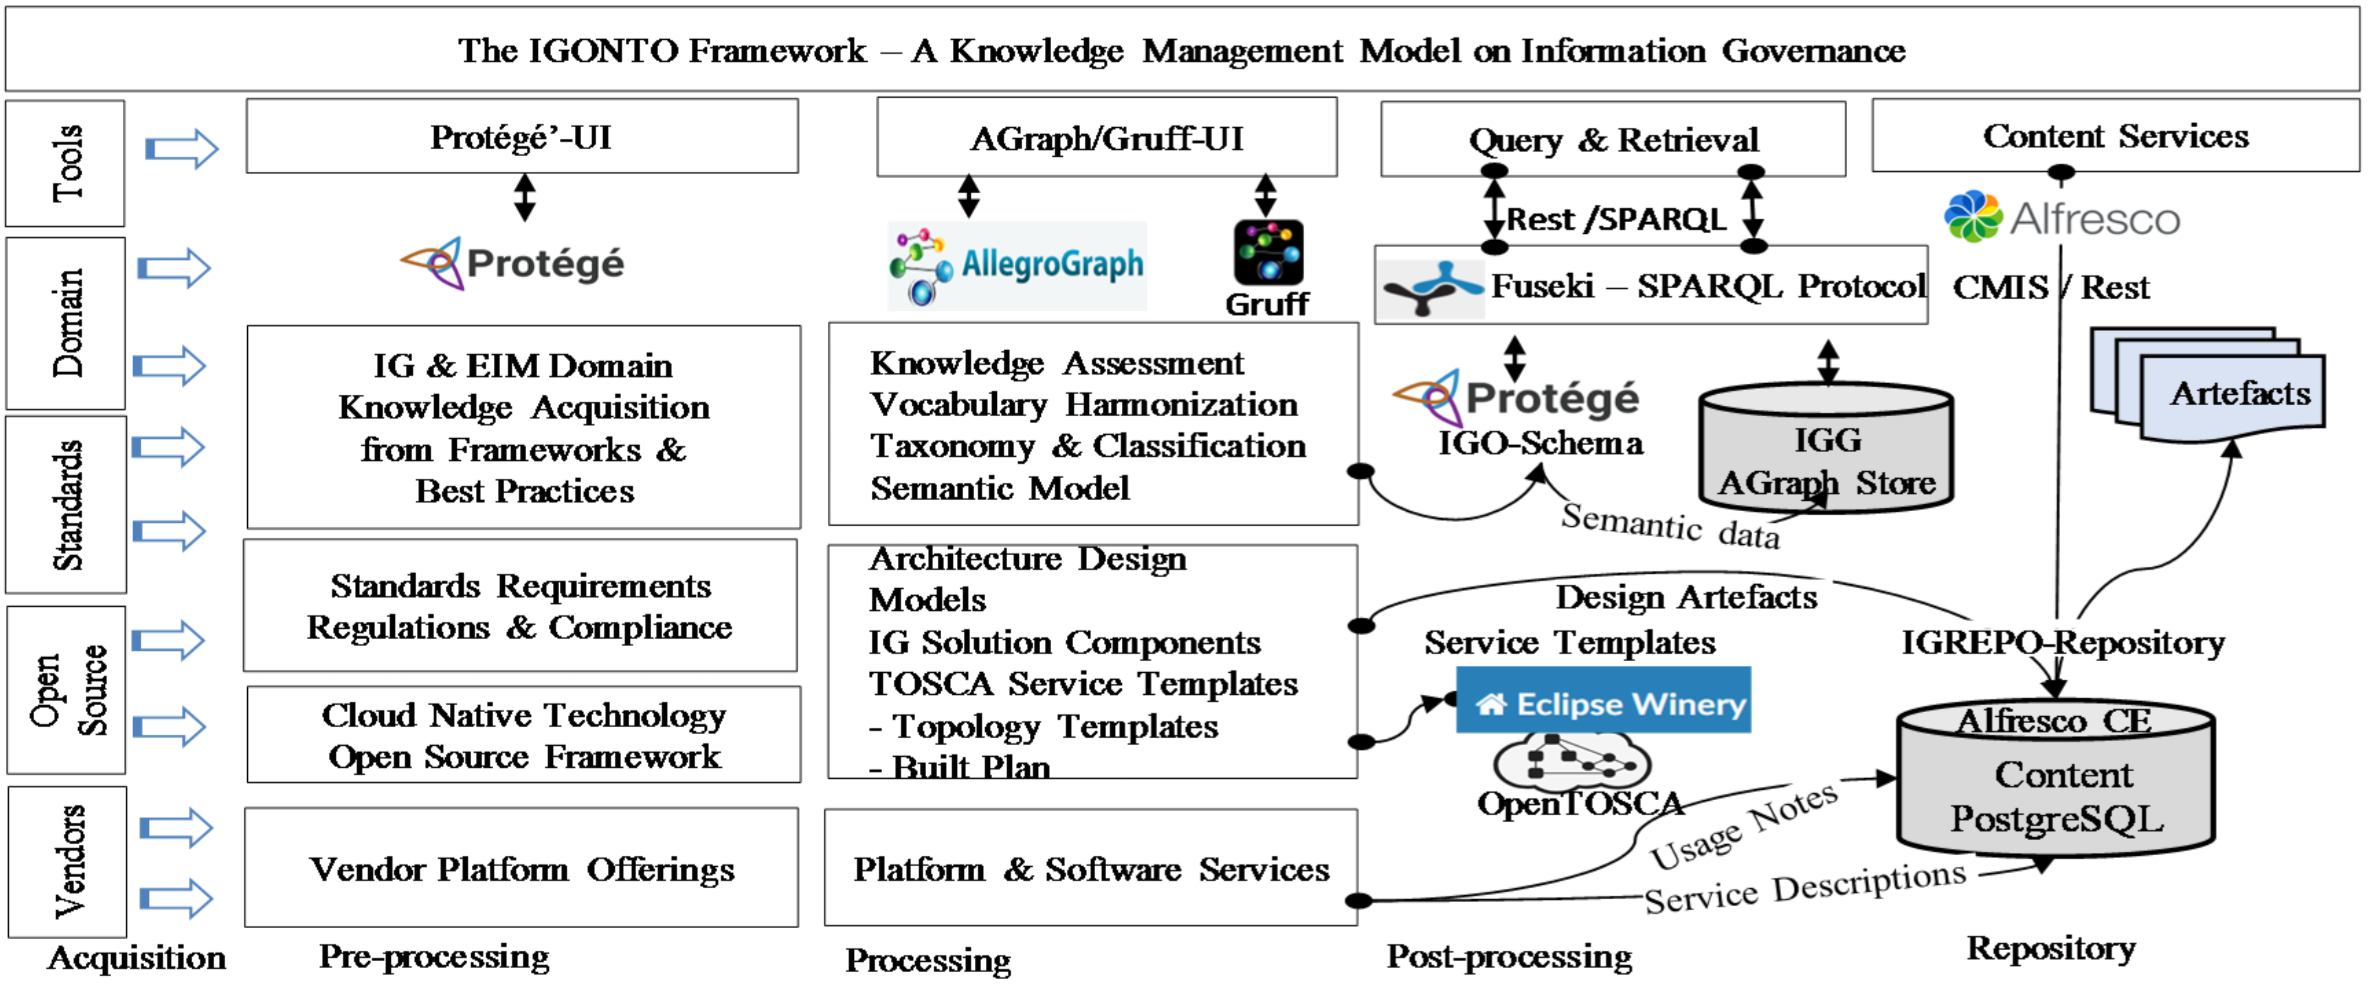
\includegraphics[width=\textwidth]{graphics/igontoFramework.png}
  \caption{The IGONTO framework \cite{IGONTO}. }
  \label{fig:igontoFramework}
\end{figure}

The IGONTO framework re-engineers the taxonomy, enhances the terms that represent core IG concepts, defines the semantic schema (IGO), and creates a graph store (IGG). The available solution components are stored in the IGREPO repository as artifacts. The framework makes domain knowledge and experience explicit and accessible through semantic queries.

The IGONTO framework (figure \ref{fig:igontoFramework}) can be explained in the context of the following five stages of information governance: Acquisition, Pre-processing, Processing, Post-processing, and Repository.

\begin{enumerate}
    \item  Acquisition: In the acquisition stage, data is collected from various sources and pre-processed to ensure its quality and relevance. The IGONTO framework provides a common and unambiguous domain vocabulary that helps to define the data sources and the pre-processing steps required to ensure data quality.
    \item  Pre-processing: In the pre-processing stage, data is classified and transformed to make it suitable for processing. The IGONTO framework helps to define the pre-processing steps required to ensure data quality and relevance.
    \item Processing: In the processing stage, data is analyzed and processed to extract useful insights. The IGONTO framework helps to define the processing steps required to ensure data accuracy and consistency.
    \item Post-processing: In the post-processing stage, data is further analyzed and processed to produce required governance information such as audit trails, statistics, and reporting needs. The IGONTO framework helps to define the post-processing steps required to ensure data accuracy and consistency.
    \item Repository: In the repository stage, data and related metadata are securely stored in an enterprise repository, typically a Content Management (ECM) system. The IGONTO framework helps to define the repository components required to ensure data security and accessibility.
\end{enumerate}

    This thesis focuses on the first two stages, where different vocabulary and taxonomy of different frameworks are combined in one common taxonomy that is implemented as an ontology.  


\chapter{Ontology Development - Prerequisites}\label{sec:prerequisites}

\section{General approach}
This section describes several general approaches of IGONTO. Section \ref{sec:ontology_hierarchy} describes the ontology hierarchy used to build IGONTO. How object properties are implemented from the structural perspektive is explained in \ref{sec:objectproperty_structure} and same goes for the datatype properties in \ref{sec:datatypeproperty_structure}.    


\subsection{Ontology hierarchy}\label{sec:ontology_hierarchy}
The IGONTO ontology consists of several sub-ontologies. Each sub-ontology describes its own subdomain within information governance. This allows the individual domains to be represented and implemented independently. 
  
\begin{figure}
  \centering
  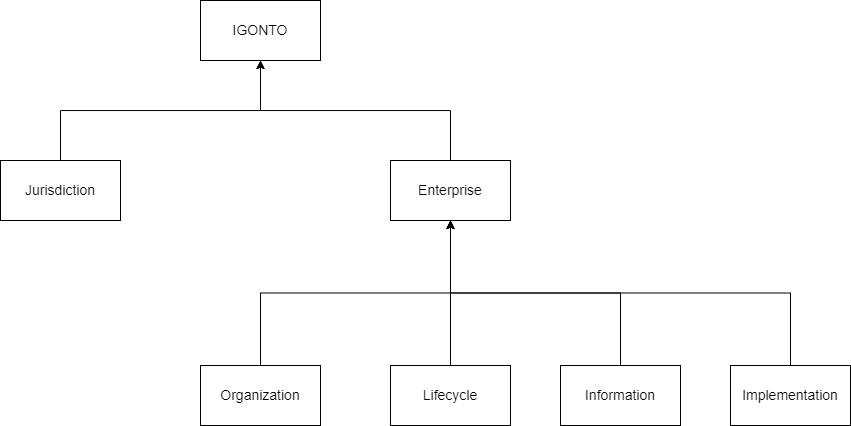
\includegraphics[width=\textwidth]{graphics/topology.PNG}
  \caption{IGONTO topology}
  \label{fig:topology}
\end{figure}

Figure \ref{fig:topology} shows the structure of the ontology. The IGONTO ontology is at the top level. This describes the finished ontology and consists of the Jurisdiction ontology and the Enterprise ontology. The Jurisdiction is responsible for covering the legal aspect of information governance, while the Enterprise ontology implements the organization, structure and relationships within an enterprise. The Enterprise ontology in turn consists of the Organization, Lifecycle, Information and Implementation ontologies. \\
Merging Organization, Lifecycle, Information and Implementation into the Enterprise ontology first, before merging it into IGONTO directly, is reasoned by the concept of reuseability. This intermediate step makes it possible to reuse the Enterprise concept in another context outside of IGONTO. Up to this point, there is no other ontology that describes an enterprise in this context. This (or parts of this) implementation can potentially be reused in other projects.\\
Each of these ontologies has its own concepts, relations, attributes and its own schema. By isolating individual sub-areas, it is possible to develop them separately from the other ontologies. This can have several advantages: 


\begin{enumerate}
    \item \textbf{Maintainability:} One advantage is definitely the maintainability. Each submodule can be developed, updated and maintained independently of the others. 
    \item \textbf{Clarity:} The clear delimitation of individual subdomains increases the clarity of the entire system. This ensures a better understanding for users and developers.
    \item \textbf{Reusability: } Small ontologies, like smaller software, are easier to reuse and embed in your own system.
    \item \textbf{Parallelism: } By isolating individual domains, it is easier to work in parallel on the overall system. 
\end{enumerate}

The division of the ontology also comes with negative aspects. These include:

\begin{enumerate}
    \item \textbf{Consistency: } It is harder to maintain an overall consistent ontology. Changes in an sub-ontology can have unwanted impact in the overall system. For that reason, it is important to develop a validation for each ontology and for the overall system, to ensure quality and consistency. 
    \item \textbf{Integration: } Maintining Sub-onotlogies need a consistent integration into the overall system. Like different branches in agile development (GitHub, etc.), it is not recommended to develop one ontology isolated for a long time. 
\end{enumerate}

To mitigate the negative aspects, a process has been designed, as outlined in \ref{sec:pipeline}, which can serve as a template for the further development of the prototype. It serves as an initial point of reference and can be modified if necessary. However, the key aspects presented there, should be kept.

\subsection{Object property structure}\label{sec:objectproperty_structure}

Object properties express relationships between instances. These relationships should be clear but simultaneously not too complicated. Reading an object property should give the user automatically insights about the object that is connected by said object property. Like reading variable names in common software should automatically give insight about the meaning and the context of the variable, increasing readability and maintainability. \\

\begin{figure}
  \centering
  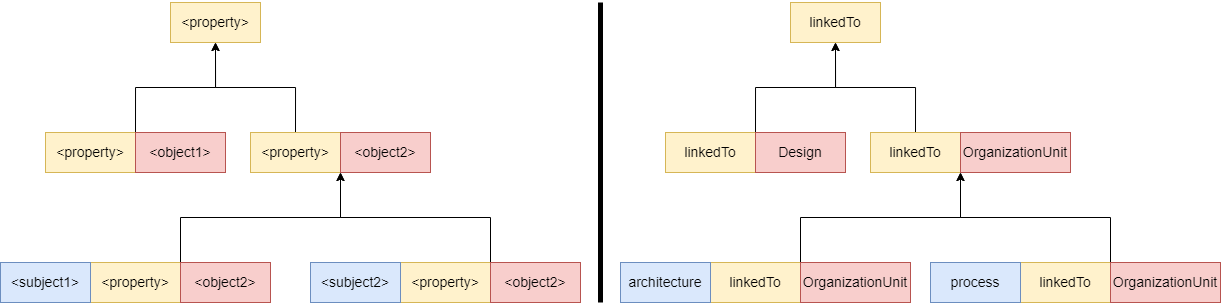
\includegraphics[width=\textwidth]{graphics/object_property_hierarchy.png}
  \caption{Object property structure}
  \label{fig:object_property structure}
\end{figure}

Therefore, object properties are also implemented in a hierarchical structure. Figure \ref{fig:object_property structure} describes the idea behind the implementation on the left side, accompanied by an explicit example from IGONTO on the right side. Every object property has a base \textit{<property>} that acts as the super property. In this example the super property is \textit{linkedTo}. This super property not linked to any instance directly, but acts as a parent to structure the properties beneath it.\\
The next level and the first possible relationships are direct children of the super property, build from the base property (\textit{linkedTo}) and the range of the class (\textit{<object1>} / \textit{Design}, \textit{object2} / \textit{OrganizationUnit}, ...), that should be connected by that object property. In case that the object class is only connected by exactly one subject class with the base property, there is no need to go further down (see \textit{linkedToDesign}). But in case that multiple subject classes (\textit{<subject1>} / \textit{architecture}, \textit{subject2} / \textit{process}, ...) connect with the same base property to the same object class, further implementation is needed.\\
If no further implementation would be done, both classes would have the same relationship, leading to possible inconsistencies or wrong interpretations within the ontology. For instance, if \textit{architecture} and \textit{process} have no other object properties or datatype properties that distinguish both classes from each other, the reasoner would interpret them as equivalent classes. On the one hand, this is semantically wrong because the concept of process does not describe the same like the concept of architecture. On the other hand, if the ontology explicitly has the rule that those classes are disjoint to each other, the reasoner would throw an error and therefore the ontology would be inconsistent. \\

\begin{figure}
  \centering
  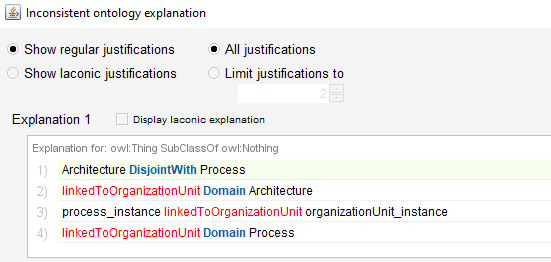
\includegraphics[width=\textwidth]{graphics/inconsistent.PNG}
  \caption{Reasoner inconcsistency example}
  \label{fig:inconsistent}
\end{figure}

Figure \ref{fig:inconsistent} visualizes the possible inconsistency and presents the reasoner's explanation. Line 1 states that both classes \textit{Architecture} and \textit{Process} are disjoint from each other. Line 2 and 4 state, that both classes are registered as the domain of the property and line 3 shows the connection of the process instance to the object. Due to these axioms, the reasoner interprets both instances as member of both classes which contradicts to the disjoint argument and therefore leading to inconsistency. Removing the disjoint argument would resolve this error, allthough it would lead to the first problem, which is not inconcistent, but semantically wrong.\\

Besides the consistency issues that are solved with this structure, the readability and maintainability are enhanced. Instances are always connected via the bottom level of the object property structure. So in the example shown in \ref{fig:object_property structure}; subject instances would be connected with \textit{linkedToDesign, architectureLinkedToOrganizationUnit, and processLinkedToOrganizationUnit}. The object for every relationship is clear, namely \textit{Design} and \textit{OrganizationUnit}, only by reading the object property name. Without these suffixes, every instance would be connected via \textit{linkedTo} and the possibility arises to not know what type the object is of. In case of \textit{linkedToOrganizationUnit}, the reader is also aware of the subject type, namely \textit{architecture} and \textit{process}. If desired, the subject could also be included in \textit{linkedToDesign}, but to reduce unwanted overhead in reasoning and querying, the subject is only included if really needed to prevent inconsistency.\\
Simultaneously, if reasoning is enabled, the query can also be implemented by only using the super property \textit{linkedTo}. There is no need to remember the exact object property, because all properties are subproperties of \textit{linkedTo} and the reasoner iterates through the whole structure. Asking what subjects are \textit{linkedTo} what objects would lead to the same set of objects like using the exact subproperties.\\

Organizing object properties in such hierarchical way not only increase consistency but also the readability and maintainability of the ontology and queries. All instances are connected in a systematic way, facilitating a clearer understanding of relationships and promoting effective knowledge representation.

\subsection{DatatypeProperty structure}\label{sec:datatypeproperty_structure}

\section{Reasoning}
This chapter encompasses the exploration of reasoning. In Section \ref{sec:what_is_reasoning}, it explains what reasoning is, the tasks it fulfills, and the parameters to consider regarding a knowledge graph in order to select the appropriate reasoning. Subsequently, Section \ref{sec:reasoning_types} introduces several reasoning methods and their characteristics. Section \ref{sec:igonto_characterization} delves into the characterization of our IGONTO's knowledge graph, and finally, Section \ref{sec:reasoning_choice} deals with the proper selection of reasoning for our use case.


\subsection{Ontology Reasoning and its Parameters}\label{sec:what_is_reasoning}
Reasoning is a fundamental aspect of ontologies, as it allows for the extraction of meaningful information and the inference of new knowledge based on the existing ontology. Ontological reasoning involves applying logical rules and algorithms to the ontology in order to derive new facts or validate existing ones \cite{Tran.2008}.\\
One of the main reasons for using reasoning in ontologies is to ensure consistency. Reasoning can detect and resolve inconsistencies within the ontology, ensuring that the knowledge represented is coherent and free from contradictions \cite{Köhler.2011}. Additionally, reasoning can be used to validate the correctness of the ontology by checking for logical errors or inconsistencies \cite{Setiawan.2019}.\\
Reasoning also enables ontology alignment, which involves finding correspondences between different ontologies to facilitate interoperability and knowledge sharing \cite{Slater.2016}. By using reasoning algorithms, ontologies can be aligned based on their logical structure and semantic relationships, allowing for the integration of knowledge from multiple sources \cite{Li.2015}.\\
Furthermore, reasoning in ontologies allows for concept subsumption, which is the ability to infer that one concept is more general or specific than another. This is particularly useful in applications such as information retrieval and search, where the ontology can be used to categorize and organize information based on hierarchical relationships \cite{Qing.2009}.

There are several reasoning methods that one can use. However, in order to determine which method is the best for one's use case, one must first consider the characteristics of a knowledge graph that play a role in the choice of the method. The following will explain key shortly aspects of a knowledge graph that are important for the choice of the right reasoning method.

\begin{enumerate}
    \item The \textit{size} of a knowledge graph can impact the efficiency and scalability of reasoning methods. Larger knowledge graphs may require more computationally intensive reasoning methods to handle the complexity and volume of data. On the other hand, smaller knowledge graphs may be more easily reasoned over using simpler methods \cite{Chen.2020}. Therefore, the size of the knowledge graph should be taken into account when selecting a reasoning method.
    \item The \textit{accuracy} of making correct inferences, and consequently, the accuracy of avoiding incorrect inferences, is also an important aspect that is used by \cite{TIAN2022100159} to distinguish reasoning methods. This raises the question of how important it is to avoid incorrect inferences and how severe the consequences can be when incorrect inferences occur.
    \item Another aspect is the \textit{frequency of data changes} in the knowledge graph and its structure. The more frequently and extensively the knowledge graph changes, the more dynamic the reasoning must be. The review by \cite{Chen.2020} explores different techniques and approaches for reasoning over knowledge graphs, highlighting the need for dynamic reasoning to handle the frequent changes in the knowledge graph.
    \item Another aspect is the need for \textit{explicit explanations of inferences} \cite{TIAN2022100159}. This raises the question of whether we only want to see the result or also the justification for why this inference was made and how transparent this justification is.
    \item The last aspect is \textit{performance}. Naturally, the reasoning method should be chosen to align with the knowledge graph, ensuring that performance is not compromised. Furthermore, there is a general decision to be made regarding whether real-time results are needed for one's use case, or whether, for example, faster results for usability reasons are desired, even if the data itself is not required in real-time.

\end{enumerate}
In conclusion, while there may be additional smaller aspects to consider, the aforementioned points encompass the most critical aspects that should be taken into account when selecting a reasoning method for a knowledge graph.






\subsection{Reasoning methods}\label{sec:reasoning_types}
This section is dedicated to introducing the most well-known reasoning methods. For this purpose, we get inspiration from the methods presented by \cite{TIAN2022100159}, which offer a comprehensive overview of various approaches to reasoning. For each method explained, we also present the pros and cons to facilitate the evaluation in the next section and determine which method is best suited for our knowledge graph.

\subsubsection{Reasoning based on logic rules}
Reasoning based on logic is further divided into two subcategories. The first subcategory is Reasoning based on \acrfull{FOL}. \acrshort{FOL} provides a formal language for representing knowledge, performing logical inferences, and serves as the basis for logical reasoning, enabling the derivation of new facts from existing ones \cite{Fitting.1990}. \acrshort{FOL} Reasoning is represented by rules which are manually defined by experts. One Example is the representation by Horn clauses, which is near to natural human language and therefore increasing the readability of said rules. Another logic-based reasoning is description logic. In this method, so-called TBoxes and ABoxes are defined. TBoxes are teminological axioms, which describe concepts and relations, and ABoxes are assertional sets, which consist of a variance of TBoxes and thus describe whole concepts. However, description logic is primarily used for validation and contributes to a consistent structure of the ontology. \\
Another logic-based reasoning method is reasoning based on statistics. The goal of this method is not to define rules by yourself, but to automatically extract and apply said rules with the help of machine learning approaches. A distinction is made between \acrfull{ILP} and \acrfull{ARM}. While \acrshort{ILP} aims to learn abstract rules from examples, \acrshort{ARM}'s goal is to detect and extract patterns in large amount and to find association rules between different attributes. \acrshort{ILP} achieves its goal by applying machine learning techniques and logic programming to automatically detect and model complex realationships in data. \acrshort{ARM} on the other hand achieves this goal by using algorithms to find said association rules that describe how different attributes are connected to each other.
\acrshort{ILP} dispenses manually defined rules and offers good reasoning via small scale knowledge graphs. \acrshort{ARM} offers high-confidence rules, is faster and thus able to handle more complex and larger knowledge graphs.\\
Reasoning based on graph structure refers to using the structure of the graph as a feature to draw conclusions. The idea is that the relationships between entities in the graph can be used to discover and infer new facts or relationships. A typical feature in a knowledge graph is the paths between entities, which play an important role in knowledge processing. This method is divided into global structured-based and local structured-based models. In the global structured-based model, the paths of the entire knowledge graph are used as a feature, which makes this method effective but also computationally expensive. On the other hand, the local structure-based model, focuses on finer granularity by examining only the narrow and local graph structure of the relationship under investigation. Therefore the computational costs are lower. 

\subsubsection{Knowledge Graph reasoning based on representation learning}
The basic idea of representation learning is to convert complex data structures into vectors. There are several approaches to this, such as the tensor decomposition approach, distance model or the semantic matching model. The tensor decomposition approach uses the possibility to model interactions between entities and relations using a three-way tenor (entity-relation-entity). \acrfull{RESCAL} is the most widely used approach. By solving the simple tensor decomposition problem, Rescal reflects the similarities of neighboring graph structures. However, \acrshort{RESCAL} is simple and, suitable for more complex graphs, needs a large amount of training data and does not give explicit explanations for rasoning results.\\

\subsubsection{Knowledge Graph reasoning based on neural network}
Knowledge Graph reasoning based on neural networks is a type of Knowledge Graph reasoning approach that uses neural networks to learn the representations of entities and relations in a Knowledge Graph and perform reasoning tasks. This approach is particularly useful for complex and multi-hop relation reasoning, where traditional logic-based reasoning methods may not be effective. Knowledge Graph reasoning based on neural network is effective for link prediction, entity classification and question awnsering but lack on performance and don not provide explicit explanations for reasoning results.


\subsection{IGONTO characterization}\label{sec:igonto_characterization}
In this section we will discuss the characterization of our Knowledge Graph regarding the parameters mentioned in \ref{sec:what_is_reasoning} to be able to choose the correct and for our use case suitable reasoning method.\\

\subsubsection{Parameter: Size}

The first parameter pertains to the size of the knowledge graph. To classify our Knowledge Graph, we need to establish what distinguishes a Knowledge Graph as small or large scale. However, defining such a threshold is challenging and cannot be stated categorically. Several factors come into play, including the number of classes, individuals, relations, attributes, and the degree of interconnection among individual instances (i.e., the quantity of relationships and attributes each instance possesses). While it is feasible to query the precise metrics of our Knowledge Graph with the assistance of Protegé, as illustrated in Figure \ref{fig:ProtegeMetrics}, there is no official reference metric that designates a Knowledge Graph as 'large' based on a specific number of instances. \\
The distance model aims to model the distance between the embeddings of the subject and object entities in the knowledge graph. By minimizing the transformation error, this type of model learns low-dimensional embeddings of all the entities and relation types in the knowledge graph.\\
The Semantic matching model uses a scoring function to determine similarity. With the scoring function, hidden semantics between entities and relations are matched and thus the validity of relation triples among these entities are measured. Becuase of the large amount of parameters, this method suffers from a high complexity. 

\begin{figure}
  \centering
  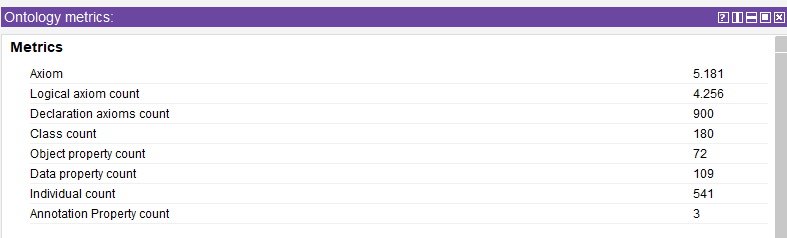
\includegraphics[width=\textwidth]{graphics/ProtegeMetrics.PNG}
  \caption{Knowledge Graph metrics. }
  \label{fig:ProtegeMetrics}
\end{figure}

However, one possible parameter could be storage space, which provides an approximate measure of the graph's size. It is also feasible to transform a relational database into a knowledge graph \cite{Virgilio.2013}. We can compare the size of the knowledge graph with that of a relational database. Currently, the required storage space for our Knowledge Graph is approximately 1 MB. A database of this magnitude is decidedly not large. Even if one were to argue that the prototype is not yet complete, the order of magnitude remains the same. This is because all articles of the \acrlong{GDPR}, as well as a significant portion of an enterprise, are implemented. Not many instances would be added, especially not in a quantity that would alter the order of magnitude in which we currently reside. Therefore, our Knowledge Graph is unequivocally on a small scale.

\subsubsection{Parameter: Accuracy}
The accuracy of the inferences plays a particularly important role in our USe case. Every inference must be correct and no inference should be too much. To do this, we make two case distinctions:\\
\begin{enumerate}
    \item In the event that an inference is omitted when it should be made, this could have significant consequences. For instance, if a company is told that it does not require certain tools or processes because the inference has not been formed. This could result in a violation of the GDPR and accordingly in a large fine. For example, the Marriott hotel chain has been fined 18.4 million euros for failing to comply with certain safety standards \cite{gdpr.2021}. Therefore, if an inference related to this standard is missing, it would not be a satisfactory implementation.
    \item In the event that an inference is formed too much and refers, for example, to a process that is not actually required, it may not lead to a legal problem, but it would necessitate the allocation of resources to implement unnecessary processes, causing economic damage.
\end{enumerate}

In both cases, inaccurate inferences would be very harmful. We cannot afford "false positives" or "false negatives". Consequently, we need a high degree of accuracy in inferences to guarantee both good and also sufficient GDPR compliance.

\subsubsection{Parameter: Frequency of Data Changes}
Here, the question must be clarified regarding how frequently new instances, relationships, or attributes are added and how often specific instances are altered in such a manner that a different structure is formed. A good indicator is the frequency of changes in the \acrlong{GDPR}. The last update to the GDPR occurred on May 25, 2018. Even ISO standards, which are designed to provide years of stability and continuity, do not undergo frequent changes. Therefore, data within the mature IGONTO Knowledge Graph is unlikely to experience frequent alterations.

\subsubsection{Parameter: Explicit Explanations of Inferences}
In our use case, an explanation of inference is useful, if not necessary. For instance if a company is told by querying the knowledge graph that it has to implement a certain tool / process, there is certainly a potential interest in finding out why this is necessary in the first place. Each additional process costs money and resources, hence making it crucial to comprehend the reasons behind the inference. Accordingly, an explicit justification is necessary.


\subsubsection{Parameter: Performance}
Of course, good performance is always desirable. Here, however, a distinction must be made between whether real-time results are needed, or whether it would be manageable to wait a few seconds. Our use case is not software that requires results in real time. How often queries are executed and how often certain queries are repeated also plays an important role.
In theory, a company may only need to execute each query once, as the ultimate result remains unchanged. Repeated queries will yield the same processes and outcomes. In this respect, performance in our knowledge graph does not play a major role and should not be the highest priority. Instead, the fulfilment of the other parameters would be much more important. Of course, it is still necessary to choose an reasoning method that balances suitable performance.

\subsection{Reasoning choice}\label{sec:reasoning_choice}
If we now take a look at the properties of the knowledge graph, it can be said that what is needed above all is a method for small-scale knowledge graphs with a high level of accuracy. The rules and inferences must be comprehensible and explainable. Although a dynamic method would also be desirable, the dynamic methods presented here have poor accuracy, no justification for the inferences and are more suitable for large scale knowledge graphs. Therefore, the reasoning method with logic-based reasoning is the right choice. \\
However, we will use the approach of choosing reasoning with first order logic for the inferences and extending them with SWRL rules. With the SWRL rule, complicated chained inferences can be determined with high accuracy. Furthermore, we will also use reasoning with description logic. In addition to that, every ontology will have an own SHACL schema to guarantee consistency and to be able to validate our ontology. 

\subsection{\acrfull{SHACL}}\label{sec:SHACL}

\subsubsection{Validation} \label{sec:validation}
\acrfull{SHACL} is a language with a focus on validating RDF graphs. Usually, \acrshort{SHACL} is implemented in a separate document, which is often referred to as a \textit{schema}. The schema consists of \textit{shapes} on which the RDF graph is validated. Each shape is a tuple \textlangle s, t, d \textrangle, where \textit{s} describes the unique \textit{id} of the shape, \textit{t} the \textit{target definition}, and \textit{d} the \textit{set of constraints} for the target. If the graph meets the constraints, it is considered \textit{valid}. In the case that the RDF graph violates a constraint in the schema, the validation report throws an error with an explanation of which constraint failed and why. Because the schema is an RDF graph itself, it does not need additional infrastructure and can even be embedded in the ontology by itself \cite{Pareti.2021}. Although usually, for maintainability and usability reasons, the schema is stored separately in a file.\\
Figure \ref{fig:shacl} shows a brief example of a \acrshort{SHACL} shape in our jurisdiction ontology. Following the first triple, which is the definition of the shape and its name, the target of the shape is defined. In our example, the target is a whole class and therefore all instances from this class (here: \textit{EU}) are considered as \textit{focus node}. There are overall four types of possible target definitions. 
\begin{enumerate}
    \item \textit{sh:targetNode}: Specifies an individual instance as the target node of this shape and its contraints. 
    \item \textit{sh:targetClass}: Specifies a class and therefore all of its instances as the target node of this shape and its contraints. 
    \item \textit{sh:targetSubjectsOf}:Specifies a property and therefore all constaints of the shape apply to all the subjects of that property.
    \item \textit{sh:targetObjectsOf}:Specifies a property and therefore all constaints of the shape apply to all the objects of that property.
\end{enumerate}

After the specification for which instances this shape is responsible, the set of constraints follows. Recursively, these constraints can be implemented as their own property shapes with their own constraints, either by defining a new shape (\textit{hasRegulationShape}) or by implementing these constraints directly. Although it is recommended to define new shapes for traceability in the validation report if invalid constraints occur. The targets of these constraints are called the "target nodes." Here, the target nodes are all instances from \textit{jurisdiction:Regulation} and the attribute \textit{rdfs:label}. The reference of a property in the original knowledge graph is defined in \textit{sh:path}. The following lines represent the constraints of the said property. For example, the constraints for the property \textit{rdfs:label} are that the datatype of the label should be a string, and the focus node must have a minimum of one label.

\begin{figure}
  \centering
  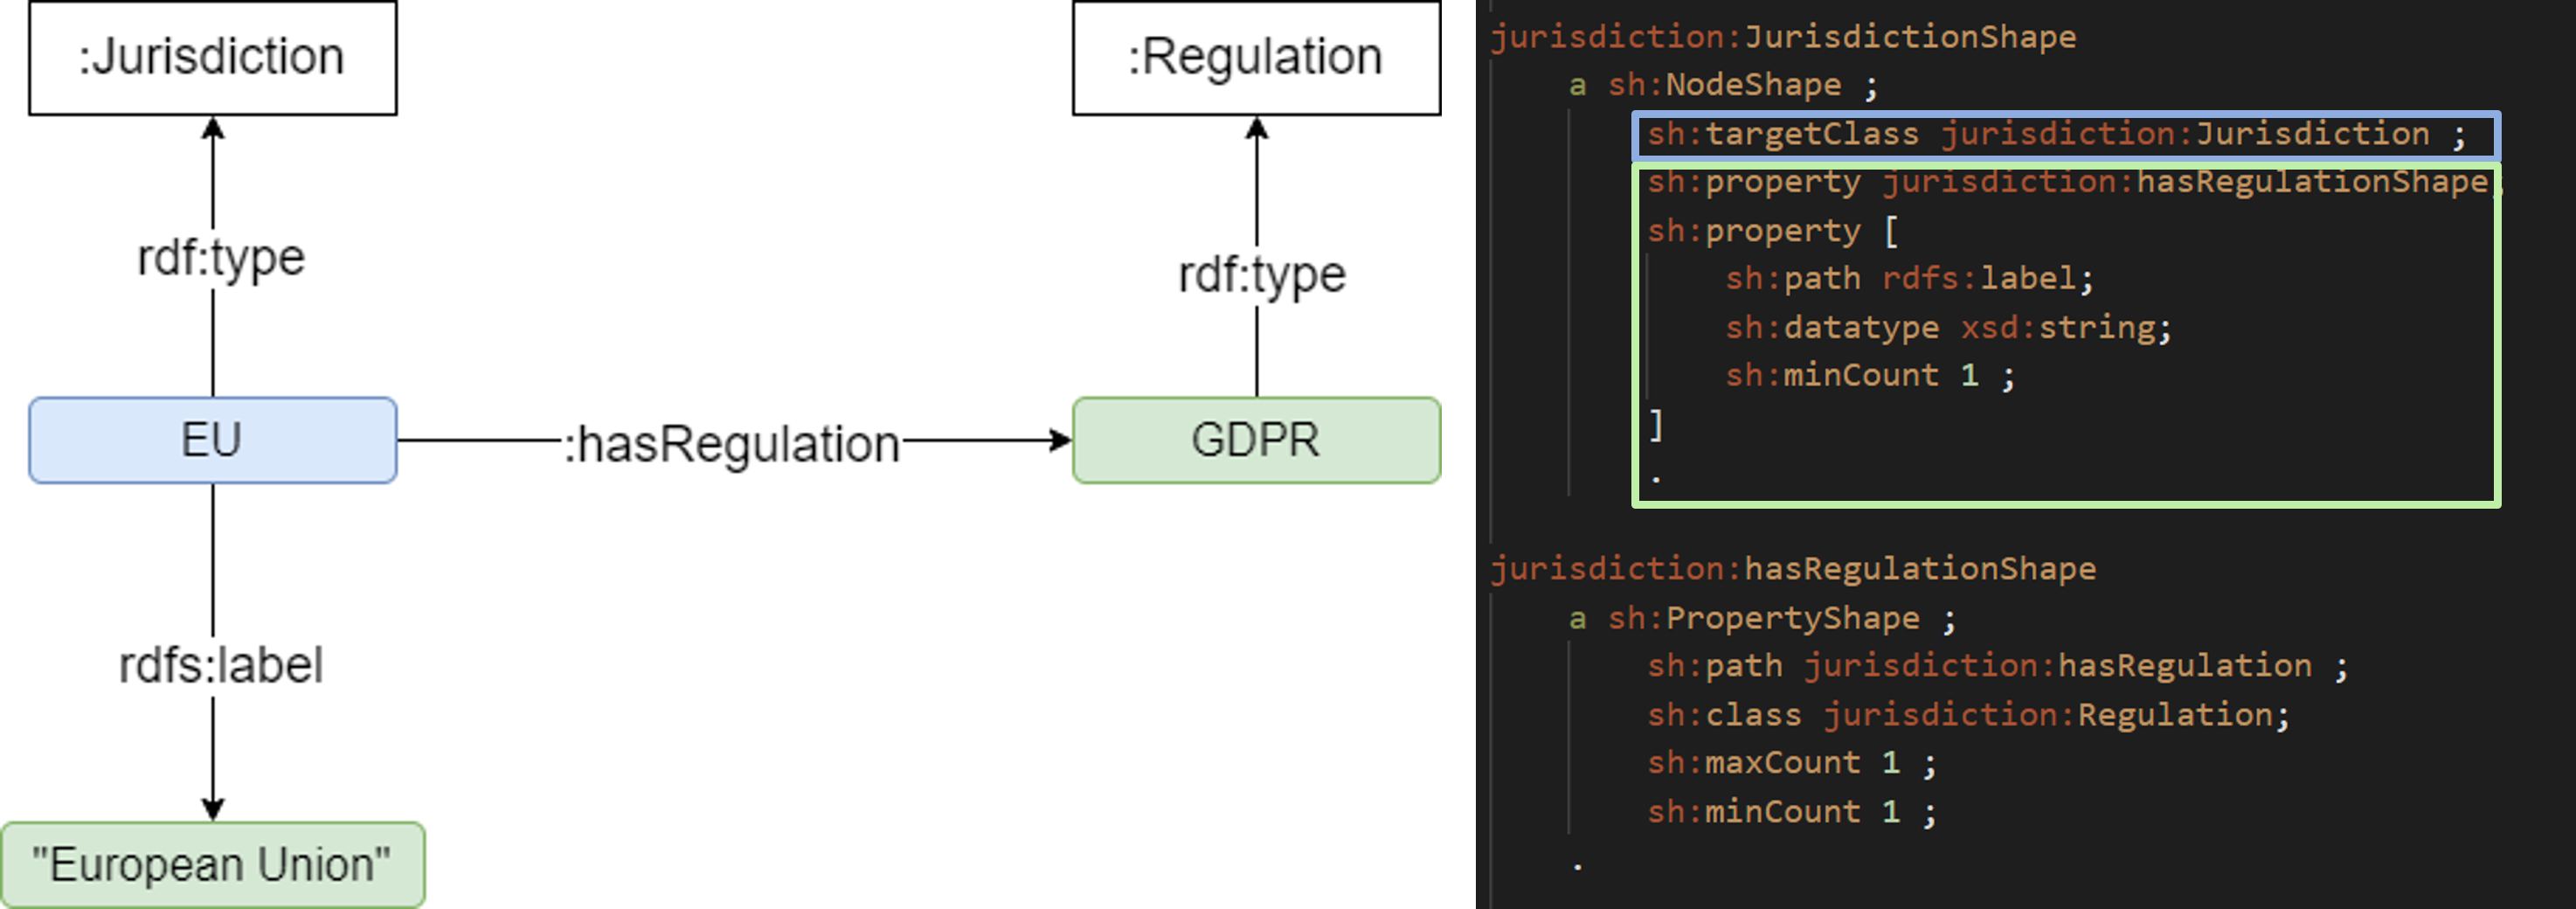
\includegraphics[width=\textwidth]{graphics/shaclExampleFinished.png}
  \caption{SHACL Example}
  \label{fig:shacl}
\end{figure}

\begin{figure}
  \centering
  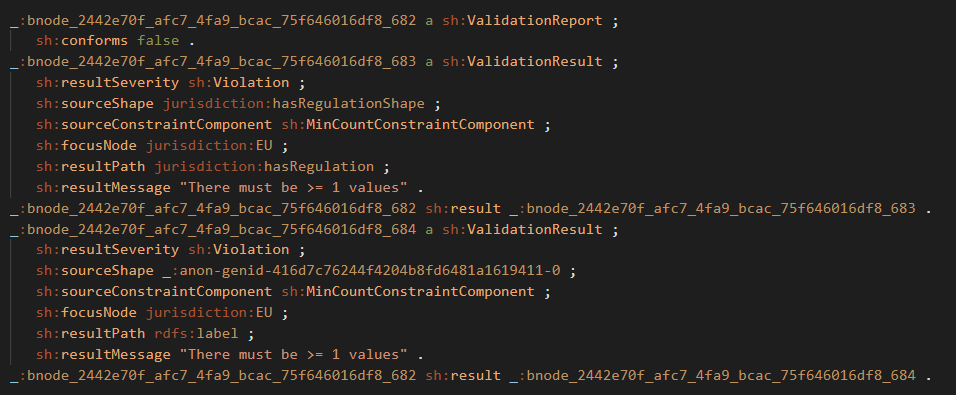
\includegraphics[width=\textwidth]{graphics/report.PNG}
  \caption{SHACL Validation Report Example}
  \label{fig:shaclValidation}
\end{figure}

Figure \ref{fig:shaclValidation} shows an example of a violation report. Here, both constraints failed. The report describes on which constraint component it failed (\textit{sh:sourceConstraintComponent}), the instance (\textit{sh:focusNode}), and the property (\textit{sh:resultPath}) that violated the constraint, along with a message explaining why it failed. This message can also be redefined for each shape and individual purpose. It also illustrates why it is useful to define new property shapes for each property. In the first violation, the \textit{sh:sourceShape} clearly indicates on which constraint, in which shape, the error occurred. On the second violation, a generic identifier for that property shape is generated because, in our schema, the property shape is anonymous and not defined. 

\subsubsection{PropertyGroups}\label{sec:PropertyGroups}
As mentioned in \ref{sec:validation}, the main purpose of \acrshort{SHACL} is the validation of RDF-graphs. In addtition of the validation, \acrshort{SHACL} can be also implemented directly into the ontology.\\
When analyzing how \acrshort{SHACL} is implemented, one can see that SHACL and its concepts are also RDF-graphs. Listing \ref{lst:shacl_shapes} shows a part of the \acrshort{SHACL} ontology. Line 2, 9 and 16 show, that a NodeShape and a PropertyShape are also classes. When defining a concrete nodeShape or a propertyShape as a \textit{sh:NodeShape / sh:PropertyShape} in a schema (see \ref{fig:shacl} JurisdictionShape / hasRegulationShape), those shapes are in reality instances from the class sh:NodeShape / sh:PropertyShape. This structure enables the ability to treat ObjecttypeProperties as instances and therefore as a subject itself by creating the corresponding propertyShape. \\



\begin{lstlisting}[style=turtle, caption={SHACL shapes definition \cite{SHACL}}]
sh:Shape
	a rdfs:Class ;
	rdfs:label "Shape"@en ;
	rdfs:comment "A shape is a collection of constraints that may be targeted for certain nodes."@en ;
	rdfs:subClassOf rdfs:Resource ;
	rdfs:isDefinedBy sh: .

sh:NodeShape
	a rdfs:Class ;
	rdfs:label "Node shape"@en ;
	rdfs:comment "A node shape is a shape that specifies constraint that need to be met with respect to focus nodes."@en ;
	rdfs:subClassOf sh:Shape ;
	rdfs:isDefinedBy sh: .

sh:PropertyShape
	a rdfs:Class ;
	rdfs:label "Property shape"@en ;
	rdfs:comment "A property shape is a shape that specifies constraints on the values of a focus node for a given property or path."@en ;
	rdfs:subClassOf sh:Shape ;
	rdfs:isDefinedBy sh: .
\end{lstlisting}\label{lst:shacl_shapes}

With these PropertyShapes and the ability to treat relationships as subjects, more information and knowledge can be created and involved in our ontology. One of the additional abilities are \textit{propertyGroups}.\\
A PropertyGroup is a concept of the \acrshort{SHACL} ontology, where PropertyShapes can be put into one thematically concept, allowing us to classify ObjectProperties, hence to improve the ontology structure and knowledge representation. This new type of knowledge can also be used in SPARQL queries. \\
To ensure consistency and a closed implementation environment, every (sub-)ontology has own PropertyGroups implemented in their \acrshort{SHACL} schema. Figure \ref{fig:PropertyGroupHierarchy} shows the concept how each PropertyGroup is implemented. The first prefix of each PropertyGroup begins with the name of the ontology. After that, the name of the PropertyGroup follows. If an ontology is a sub-ontology of annother, the corresponding PropertyGroup of that ontology will also be grouped into the super-ontology PropertyGroup. For instance, the PropertyGroup OrganizationInversePathPropertyGroup will be part of the EnterpriseInversePathPropertyGroup which will be part of the overall InversePathPropertyGroup that is implemented on the top level IGONTO ontology. Listing \ref{lst:shacl_propertyGroup} shows how a PropertyGroup is implemented in the \acrshort{SHACL} ontology. Like the PropertyShape and the NodeShape, a PropertyGroup is also a \textit{rdfs:Class}.  

\begin{lstlisting}[style=turtle, caption={SHACL PropertyGroup definition \cite{SHACL}}]
sh:PropertyGroup
	a rdfs:Class ;
	rdfs:label "Property group"@en ;
	rdfs:comment "Instances of this class represent groups of property shapes that belong together."@en ;
	rdfs:subClassOf rdfs:Resource ;
	rdfs:isDefinedBy sh: .
\end{lstlisting}\label{lst:shacl_propertyGroup}

Therefore the implementation of the InversePathPropertyGroup example is implemented like shown in Listing \ref{lst:shacl_propertyGroupImplementation} on the top level IGONTO ontology. Thus, in the enterprise ontology the declaration of the igonto:InversePathPropertyGroup sublass relation is missing, to ensure the concept of semantically self-containement mentioned before. Recursively, same goes for the organization ontology with the enterprise:EnterpriseInversePathPropertyGroup. 

\begin{lstlisting}[style=turtle, caption={SHACL PropertyGroup definition \cite{SHACL}}]
igonto:InversePathPropertyGroup 
        a sh:PropertyGroup .

enterprise:EnterpriseInversePathPropertyGroup 
        a sh:PropertyGroup ;
        rdfs:subClassOf igonto:InversePathPropertyGroup .

organization:OrganizationInversePathPropertyGroup 
        a sh:PropertyGroup ;
        rdfs:subClassOf enterprise:EnterpriseInversePathPropertyGroup .
\end{lstlisting}\label{lst:shacl_propertyGroupImplementation}

\begin{figure}
  \centering
  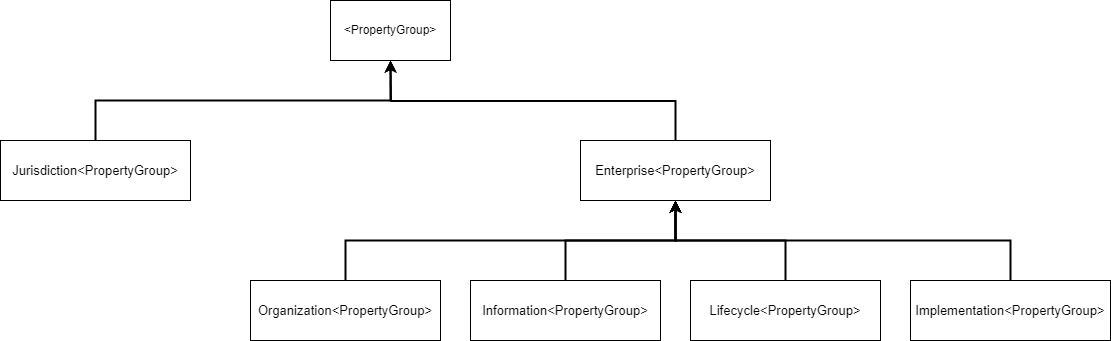
\includegraphics[width=\textwidth]{graphics/GroupHierarchy.drawio.png}
  \caption{PropertyGroup hierarchy implementation}
  \label{fig:PropertyGroupHierarchy}
\end{figure}

PropertyGroups have several positive impacts on the ontology which include: \\

\begin{enumerate}
    \item \textbf{Maintainability: }\\
    Grouping helps the developer to combine constraints on several ObjectProperties simultaneously. Each ObjectProperty within a group inherits the constraints defined in that group, making it easier to maintain these constraints and reducing the overall lines of code. 
    \item \textbf{Clarity: }\\
    Grouping can be particularly helpful when, for instance, it is not clear whether the connection of an ObjectProperty is generated via inference or statically implemented and always present. PropertyGroups can inform the developer or user about the purpose of the ObjectProperty, leading to a clearer understanding of the overall system.
    \item \textbf{Better expression: }\\
    PropertyGroups can provide a more powerful knowledge by expressing the meaning of an ObjectProperty. For instance, when the ObjectProperty explicitly indicates that there should be no connection between two instances. Because ontologies operate under the open-world assumption, a nonexistent connection cannot be interpreted as an explicitly unwanted connection. By grouping ObjectProperties within a \textit{NegativeObjectPropertyGroup}, it becomes possible to treat the ObjectProperty as a relationship that explicitly denotes the absence of a link between those two instances.
    \item \textbf{Useability: }\\
    Implementing PropertyGroups can enhance usability in query writing. For example, when a query should only include inferences or negative ObjectProperties from an instance, having groups makes filtering easier. Without them, every unwanted relationship must first be explicitly known by its name, and secondly, also by its meaning. With PropertyGroups, the query can be easily implemented by filtering out the members of a group that represents that specific semantic meaning.
\end{enumerate}

Three PropertyGroups have been implemented to improve the structure of the ontology. Each one serves a different purpose and is used differently. 

\subsubsection{InversePath- \& PathPropertyGroup:}

\subsubsection{InferenceObject- \& NormalObjectPropertyGroup:}

\subsubsection{NegativeObject- \& PositiveObjectPropertyGroup:}



\section{Ontology Fusion}

\begin{figure}
  \centering
  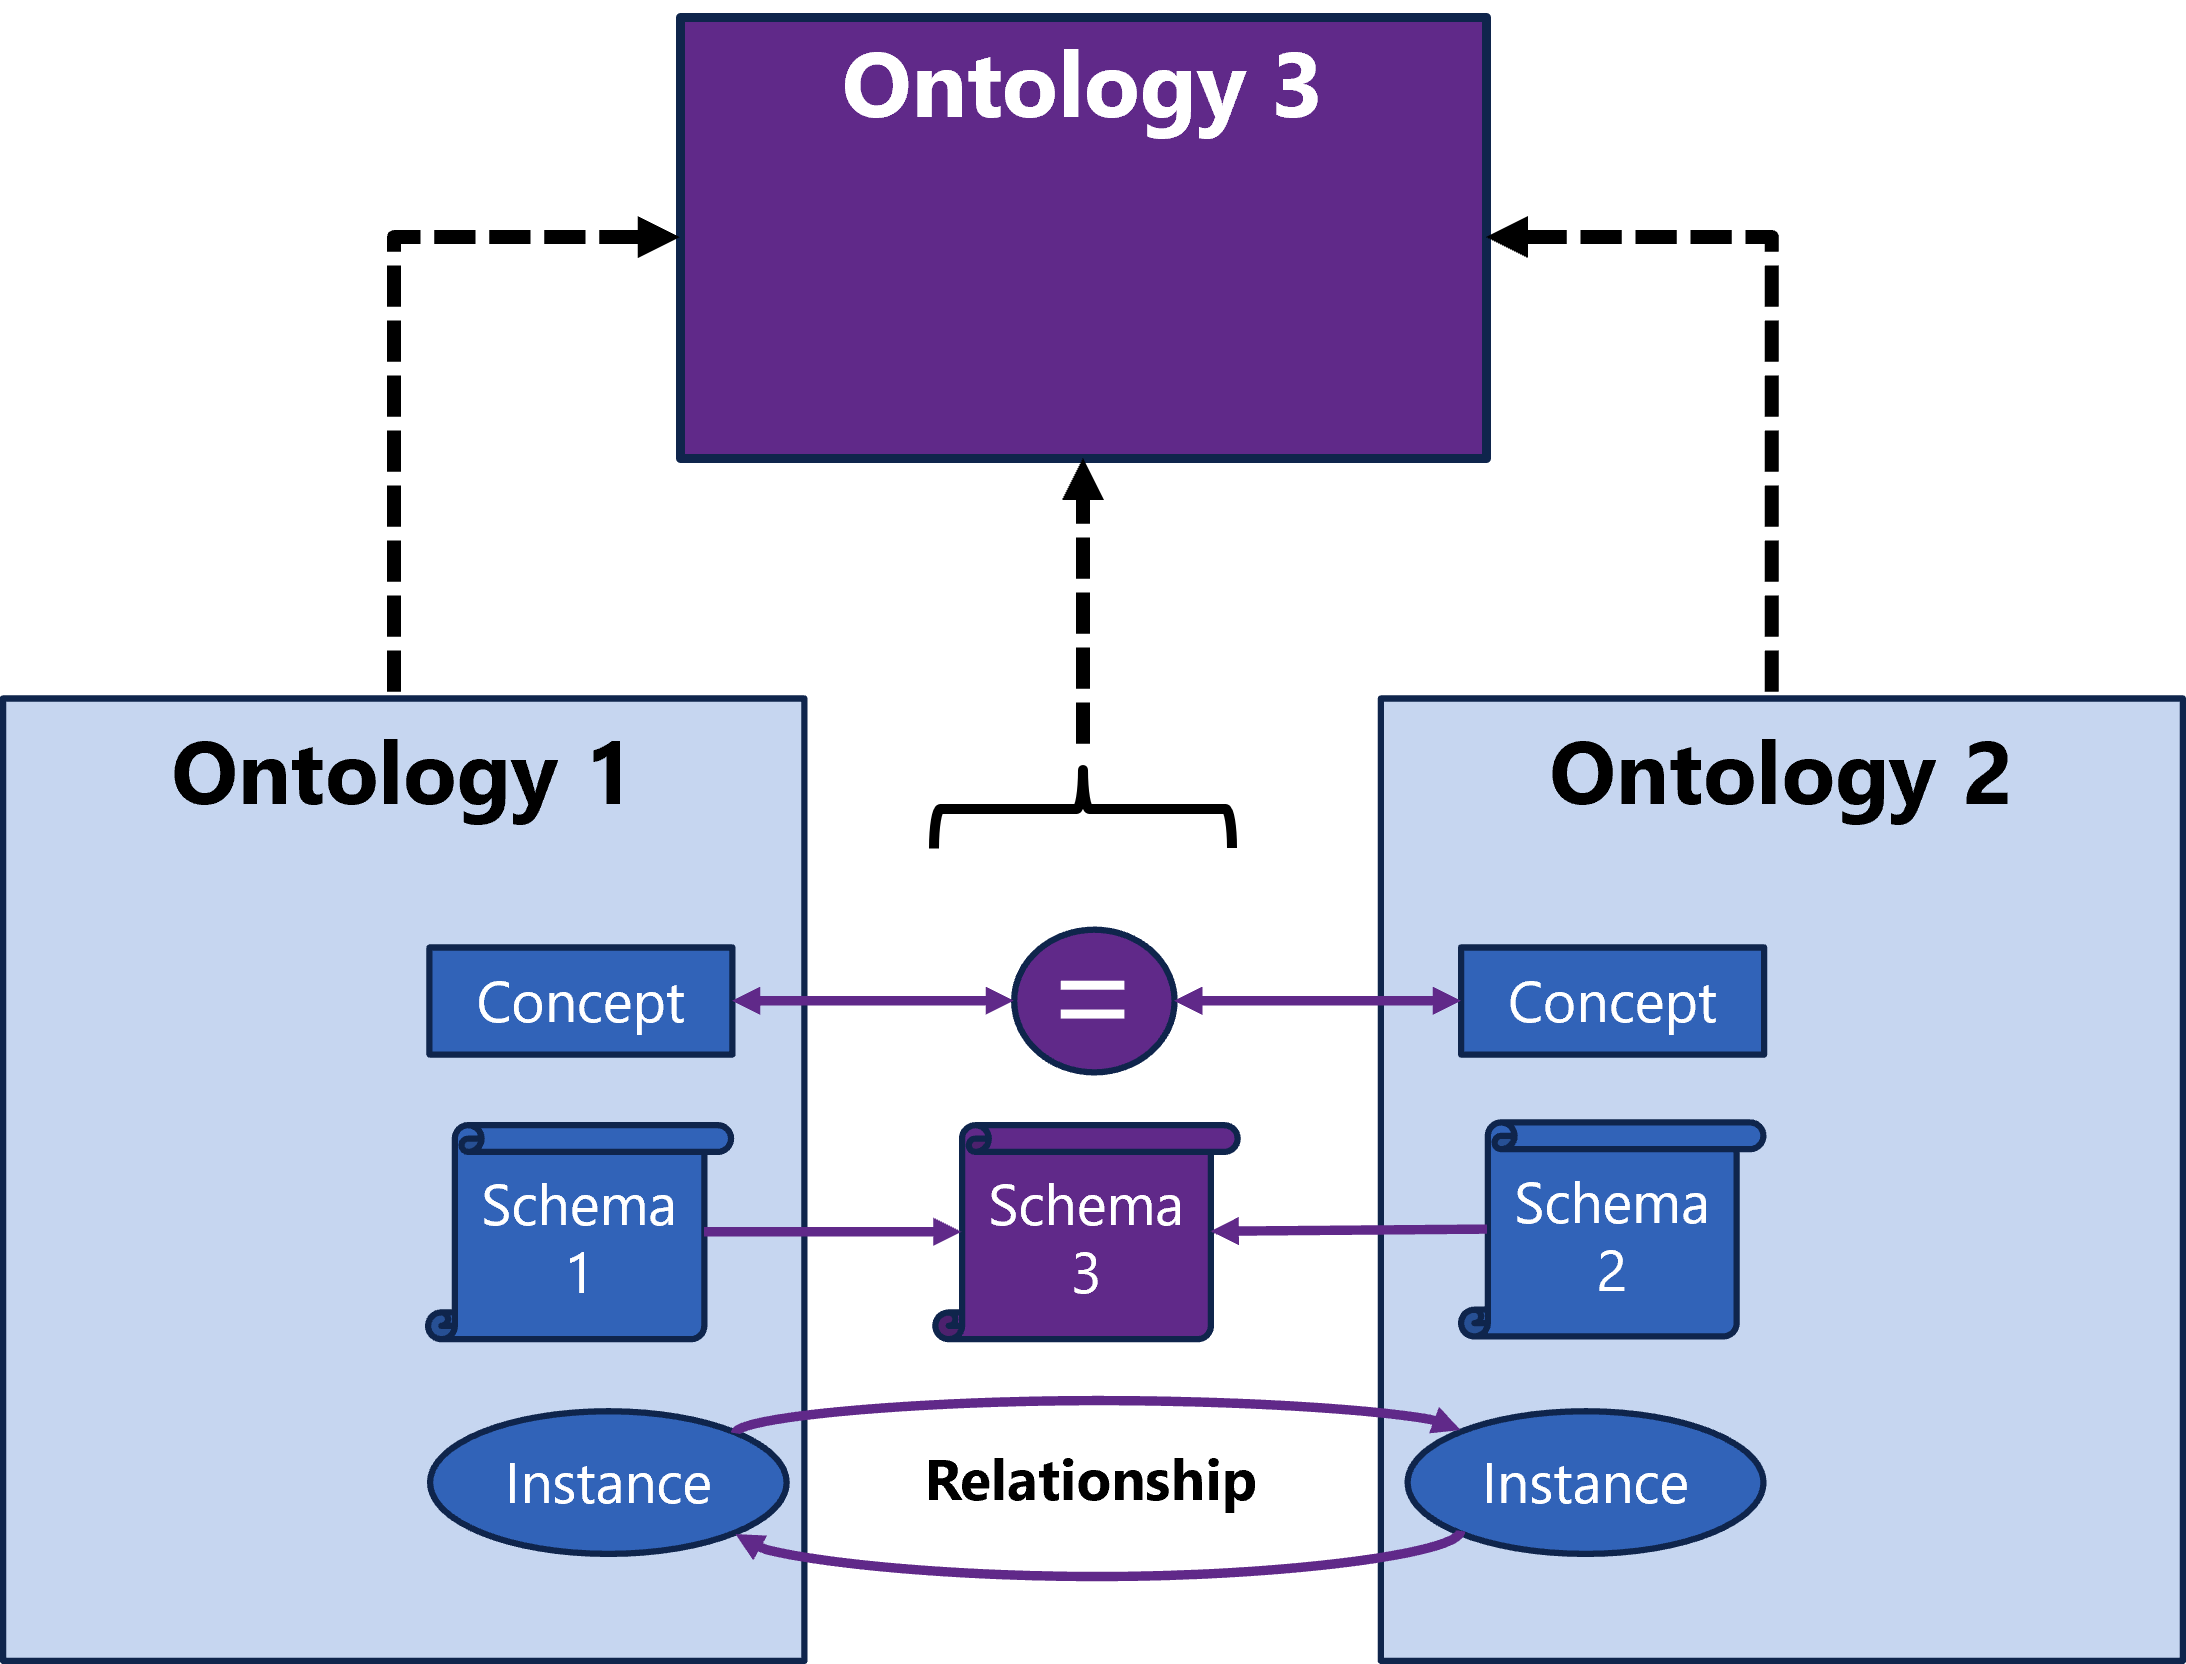
\includegraphics[width=\textwidth]{graphics/ontologyFusion.png}
  \caption{Ontology fusion}
  \label{fig:fusion}
\end{figure}

Although splitting the ontology has some advantages, these ontologies must be brought together in such a way that they work without errors in the overall system. The merging of ontologies is shown schematically in Figure \ref{fig:fusion}. It describes two different ontologies Ontology 1 and Ontology 2 with their own concepts, schemas and instances. The merging is regulated differently. \\

\subsection{Concept fusion}\label{sec:concept_fusion}

In our case, we always have at least one class as an intersection between two ontologies. This is implemented as a concept in both. These two classes describe the same concept, but either one of them is meant to be an abstract class of the other or both of describe the same thing, but in a different point of view. \\

\begin{figure}
  \centering
  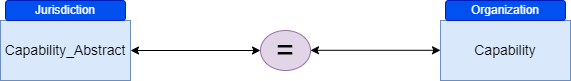
\includegraphics[width=\textwidth]{graphics/abstact_fusion.drawio.png}
  \caption{Example fusion of abstract classes}
  \label{fig:abstact_fusion}
\end{figure}

Figure \ref{fig:fusion_same} relates to the fusion of two classes where one of them is implemented as abstract, based on the example of the class \textit{Capability}. Here, the original Capability class is implemented in the Organization ontology. The significance of this class lies in the fact, that it bridges the Jurisdiction with the Organization ontology. In both cases, description logic has to be implemented from the Jurisdiction and the Organization point of view. Therefore, the implementation of an abstract class in Jurisdiction that describes the same concept from the same meaning is needed. The \textit{Capability\_Abstract} class enables the implementation of description logic from the Jurisdiction side, whereas the description logic from the organizational side is implemented on \textit{Capability}. With this approach, both ontologies are inherently consistent with the ability to implement their description logic to the connecting class. When setting both classes equal on the top ontology, both classes inherit the description logic from each other. Without this approach, the description logic would have to be implemented manually on top level, therefore decreasing the maintainability and making both classes dependent on the top level description logic implementation. If a class is meant abstractly, it will have the suffix \textit{\_Abstract} in its URI. \\


\begin{figure}
  \centering
  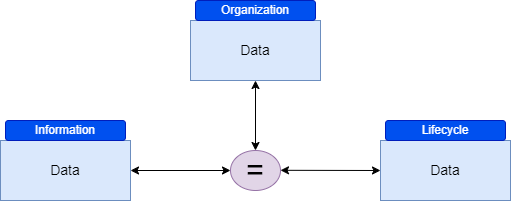
\includegraphics[width=\textwidth]{graphics/example_concept_fusion_same_meaning.drawio.png}
  \caption{Example fusion of classes with different a point of view.}
  \label{fig:fusion_same}
\end{figure}

An example for the fusion of classes that share the same concept but seen in a different point of view is shown in figure \ref{fig:fusion_same}. While the name of the class \textit{Data} is the same, the perspective from where this class is seen differentiates in every ontology. In the Information ontology, data is described in terms of its concrete value, the organizational aspect details which departments are responsible for maintaining data, and the Lifecycle ontology places it within the context of a Record lifecycle. These classes will also be set equal on top level.

\subsection{Schema fusion}
The schema fusion describes how the \acrshort{SHACL} validation schema from two different ontologies are brought together. As already mentioned in \ref{sec:SHACL}, every ontology has its own \acrshort{SHACL} validation schema implemented including its own PropertyGroups. These validation schemas can also be used on the top level ontology. Therefore combining two or more schemas is limited these implementations: 

    \begin{figure}
      \centering
      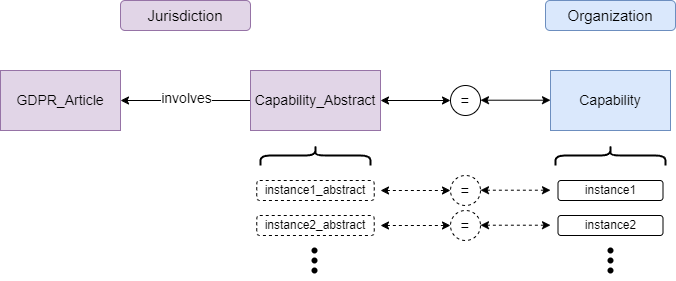
\includegraphics[width=\textwidth]{graphics/schema_concept_fusion.drawio.png}
      \caption{Schema fusion from absrtact classes example,}
      \label{fig:schema_fusion_same}
    \end{figure}
\begin{enumerate}
   \item \textbf{Abstract classes with their non-abstract equivalents:} \\
    As discussed in Section \ref{sec:concept_fusion}, one necessary measure to combine ontologies is the implementation of abstract classes in one ontology. Although the description logic of the abstract class is implemented in both ontologies, its validation is not. This decision is justified by the fact that no instances will be generated for the abstract class. \\
    To revisit the example mentioned earlier, Figure \ref{fig:schema_fusion_same} illustrates the implications if instances were also implemented in the abstract class. \textit{Capability\_Abstract} is implemented in the ontology Jurisdiction, as mentioned previously. While it is theoretically possible to implement abstract instances, doing so would allow validation of the \textit{involves} relationship between \textit{Capability\_Abstract} and \textit{GDPR\_Article}. However, it would be necessary to establish equivalence between every abstract instance and its non-abstract variant. This would result in more implementation requirements than simply validating the \textit{involves} relationship at the top-level schema. Additionally, each instance would have an unnecessary abstract duplicate, leading to unnecessary overhead in terms of storage space and query performance. \\
    Despite this overhead, the concept of the abstract class is only implemented to later connect both ontologies. Semantically, it is not crucial for the subontology Jurisdiction, and therefore, validation at the bottom level is not needed. So to still validate the \textit{involves} relationship in the overall system, the validation of relationships with abstract classes is done on top level. 
    \item \textbf{PropertyGroups:} \\
    As mentioned in \ref{sec:PropertyGroups}, every ontology has its own PropertyGroups. In order to utilize PropertyGroups from all ontologies simultaneously, these PropertyGroups become members of another PropertyGroup at the top-level schema, as shown in code snippet  \ref{lst:shacl_propertyGroupImplementation}. Those top-level PropertyGroups are implemented on the top-level schema and their members of the sub-ontologies are allocated accordingly to the correct group.
    \item \textbf{SWRL rules:} \\
       SWRL rules are implemented exclusively at the top level, as they integrate multiple classes and relationships across different ontologies. Consequently, these rules and their corresponding inferences are validated at the top-level schema.
\end{enumerate}

Apart from these implementations, the rest of the validation schema from every sub-ontology can be used exactly as they are to validate their part.

\subsection{Instance connection}

This implementation is reasoned by the abstract classes. As already mentioned, the implementation of instances for abstract classes leads to unwanted and unnecessary overhead. Returning to the example in Figure \ref{fig:schema_fusion_same}, the description logic for \textit{Capability} is automatically carried over, including the \textit{involves} relationship. However, explicit connections between instances are not automatically established. So in this case, the connection between the instances from \textit{Capability} and \textit{GDPR\_Articles} have to be connected via the \textit{involves} relationship to meet the description logic expectations. The same principle applies to any connection between a regular class and its abstract counterpart, where the non-abstract variant is implemented in another ontology, along with their respective instances.



\chapter{IGONTO development}

After the illustrating various general approaches and desgin decisions in the the development of IGONTO, this chapter describes the concrete implementation. Every subontology will be presented, along with the fusion of the whole system including the development of validation, description logic and \acrshort{SWRL} rules. The concepts, general classes and their relationship are based on previous work from \cite{IGONTO}. This chapter focuses on the specific implementation of these concepts combined with the general approaches mentioned in chapter \ref{sec:prerequisites}. \\
Each subontology will include a visual representation. However, these visualizations will be theoretically incomplete. As previously mentioned, every relationship has an inverse relationship. To avoid overloading the visual representation, only the top-down approach will be visualized and the inverse graph will be referenced in the appendix of this thesis. Additionally, for the same overloading reasons, the attributes of each class, if available, will be explained in the textual description. Although some ontologies have SWRL rules that only influence connections within their domain, the discussion of all \acrshort{SWRL} inferences will be included in a seperate section at the end of this chapter. This structure is chosen beacause the validation and implementation of all SWRL inferences occur at the top level, enhancing the ovarall structure and organization. Some classes are highlighted in green. This indicates that they contain subclasses, but are excluded from the overall visualization to enhance clarity. These subclasses do not have other relationships than the corresponding superclass. Therefore, they are not critical for the overall view and are explained in more detail in the textual description. Table \ref{tab:legend} explains how relationships and the description logic between classes are implemented in the following visualizations. \\

\begin{table}
\centering
\begin{tabular}{ 
  |>{\centering\arraybackslash}m{.5\textwidth}
  |>{\raggedright\arraybackslash}m{.4\textwidth}| 
}
\hline
\textbf{Visualization} & \textbf{Explanation} \\ \hline
\vspace{5pt}
{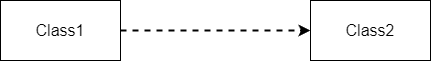
\includegraphics[width=0.48\textwidth]{graphics/Graph Legend/subclass.drawio.png}} & The dashed arrow symbolizes a subclass relation. In this case, \textit{Class1} is a \textit{subclass} of \textit{Class2}. \\ \hline
\vspace{5pt}
{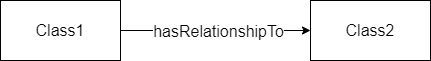
\includegraphics[width=0.48\textwidth]{graphics/Graph Legend/relation.drawio.png}} & If the arrow is not dashed, it indicates a relationship from one class to another. The relationship name is written above the arrow. In this case, \textit{Class1} has a \textit{relationship} to \textit{Class2}. \\ \hline
\vspace{5pt}
{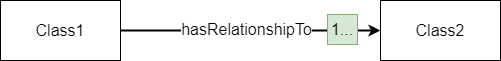
\includegraphics[width=0.48\textwidth]{graphics/Graph Legend/DL2.drawio.png}} & On every relationship arrow, certain entities are noted. These entities explain the description logic behind the relationship. If the entity has a 1 with dots, the description logic keyword 'some' is used, indicating that the subject of this relationship is connected to at least one instance from the object class. \\ \hline
\vspace{5pt}
{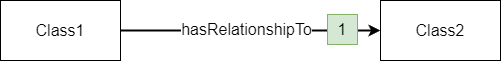
\includegraphics[width=0.48\textwidth]{graphics/Graph Legend/DL3.drawio.png}} & If the entity has a 1 without dots, the description logic keyword 'exactly' is used, indicating that the subject of this relationship is connected to exactly one instance from the object class. \\ \hline
\vspace{5pt}
{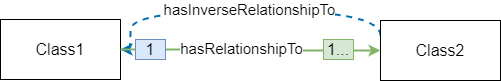
\includegraphics[width=0.48\textwidth]{graphics/Graph Legend/DL1.drawio.png}} & Every relationship has a corresponding inverse relationship that connects the subject and the object in the opposite direction. For clarity, inverse relationships are not shown in the graph, but they are practically always present. Sometimes the description logic differs in the opposite direction. To still show the inverse description logic, the entity number of the inverse relationship (here, the blue 1) is included. \\ \hline  
\end{tabular}
\caption{Graph legend}
\label{tab:legend}
\end{table}
 


\section{Jurisdiction Ontology}\label{sec:jurisdictionOntology}
The jurisdiction ontology is at the top level and encompasses the jurisiction domain of a government, its regulations and bridges the path between jurisdiction and the enterprise. Figure \ref{fig:jurisdictionVisualization} visualizes the concept level. As it connects the jurisdiction and the enterprise domain, several abstract classes are implemented (see section \ref{sec:concept_fusion}). Each abstract class is colored blue and its origins lay in the organization ontology.\\

The \textit{Enterprise} represents a business or organization that \textit{operates in} one or more \textit{Countries}. Every \textit{Country} \textit{belongs to} a \textit{Jurisdiction}, which is a legal entity of a region and has the authority to govern and legislate within its boundaries. A \textit{Jurisdiction} \textit{has} a \textit{Regulation} and \textit{Countries} are \textit{regulated by} this \textit{Regulation}, which establishes and enforces rights and obligations for enterprises. Every \textit{Regulation} \textit{requires} an enterprise \textit{Strategy} to achieve compliance and a \textit{Program} with specific initiatives and projects for said compliance. \textit{Country} has two subclasses \textit{US} and \textit{EU}, to connect countries with the right jurisdiction. Countries in the EU must comply with \acrshort{GDPR}, while states in the US need to comply with various federal and state laws, each serving a different purpose. In the IGONTO prototype, we developed information governance based on \acrshort{GDPR}. Therefore the \textit{European Union} is implemented as a subclass of \textit{Regulation} with further subclasses implementing the structure of \textit{GDPR}. \textit{GDPR} is representative for its Regulation and \textit{includes} \textit{GDPR Articles}. The GDPR has 11 \textit{Chapters}, each \textit{including} a varying number of \textit{Articles}. A total of 99 articles form the foundation of GDPR. Every \textit{Article} \textit{includes} \textit{Keywords}, to quickly summarize the intention behind each article. \\

Associations like ARMA or CGOC, based on GDPR, have created \textit{Capabilities} that try to describe how to be compliant. While ARMA concentrates on implementing the GDPR Principles, CGOC defines capabilities in a functional process way. Because they describe GDPR, every \textit{Capability} \textit{involves} some \textit{GDPR Articles}. Because these associations describe compliance from a different point of view, it is challenging to identify commonalities between them. Therefore we connect these capabilities with more general defined \textit{Rights} and \textit{Obligations} using \acrshort{SWRL} inferences to form a unified set of \textit{Requirements}. This is realized by the fact that every of these classes \textit{involves} \textit{GDPR Articles}. The exact implementation is explained in the separate section \ref{sec:SWRL}, which deals with all \acrshort{SWRL} inferences in this ontology.  Originally, these capabilites are implemented in the organization ontology, but also abstractly implemented  here because they are based on GDPR and its articles.  \\



\begin{figure}
  \centering
  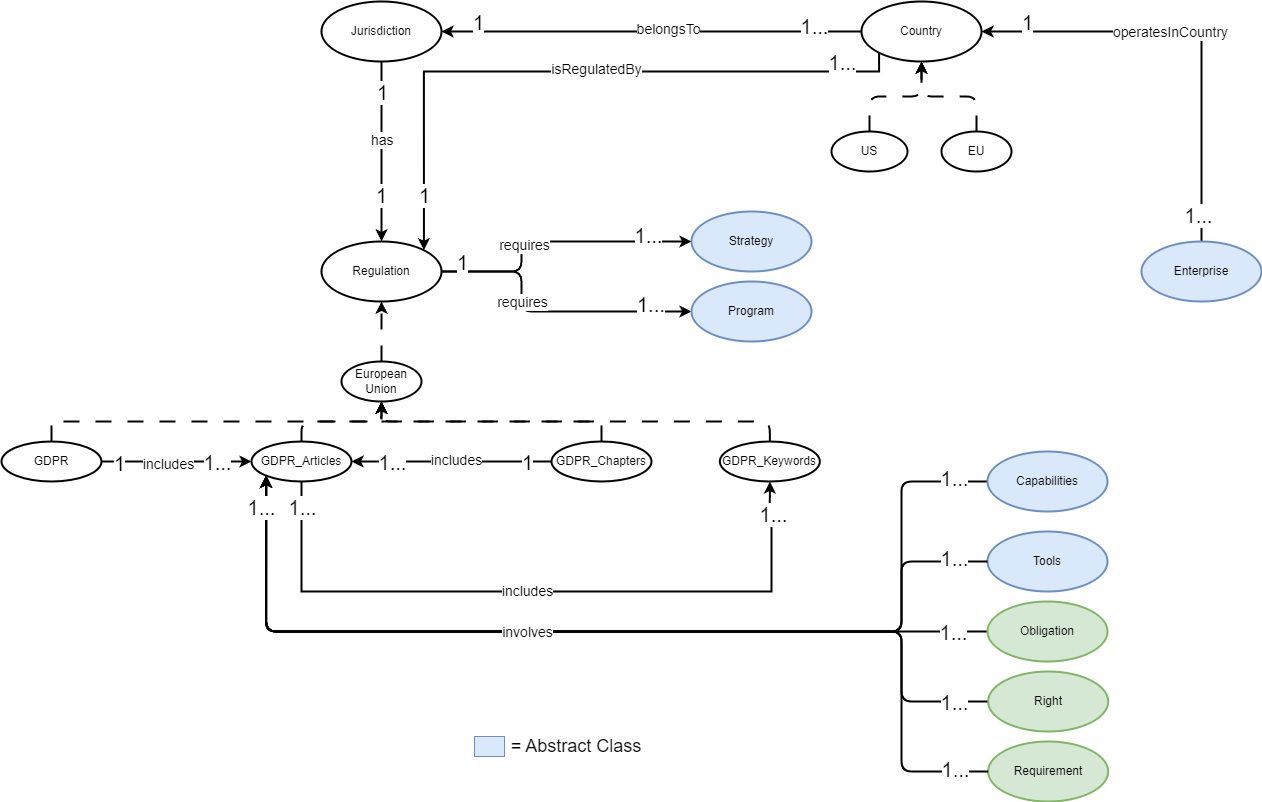
\includegraphics[width=\textwidth]{graphics/jurisdiction.drawio.png}
  \caption{Visualization of the jurisdiction ontology.}
  \label{fig:jurisdictionVisualization}
\end{figure}

\textit{Obligations} and \textit{Rights} include subclasses, each describing a specific obligation/right. Because Obligations and Rights are fundemantal for the connection between the (non)-functional \textit{Requirements} and the \textit{Capabilites}, each connection to the \textit{GDPR Articles} involve an annotaion property with a citation or explanation, why the article is involved in this obligation or right instance. Figure \ref{fig:annotationExample} illustrates this approach based on the \textit{Obligation To Ensure Integrity Of Data Instance}. \textit{Article 5} is involved in this obligation and the explanation is added as a comment to the object property as a citation from \textit{Article 5}.

\begin{figure}
  \centering
  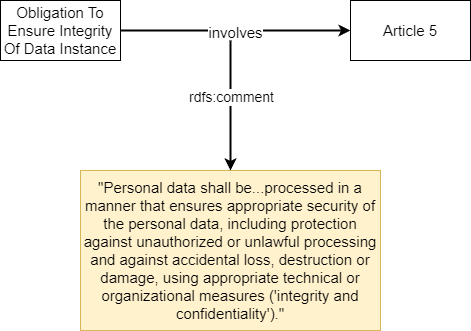
\includegraphics[width=0.5\textwidth]{graphics/annotation.drawio.png}
  \caption{Visualization of annotation property.}
  \label{fig:annotationExample}
\end{figure}

 Table \ref{tab:subclasses} shows the further taxonomy of \textit{Obligations}, \textit{Rights} and \textit{Requirements}. The intention of each \textit{Obligation}, \textit{Right} and \textit{Requirement} can be derived from the class name itself. \\
Additionally, obligations, rights and requirements are semantically grouped, if possible. These include: \\

\begin{itemize}
    \item Obligations for the Data Controller
    \item Obligations for the Data Processor
    \item Data Subject rights
    \item Functional Requirements
    \item Non-Functional Requirements
\end{itemize}

\begin{table}
\centering
\begin{tabular}{ 
  |>{\raggedright\arraybackslash}p{.2\textwidth}
  |>{\raggedright\arraybackslash}p{.2\textwidth}
  |>{\raggedright\arraybackslash}p{.5\textwidth}| 
}
\hline
\textbf{Superclass} & \textbf{Subclass level 1} & \textbf{Subclass level 2} \\ \hline
\textbf{Obligation} & Data Controller Obligation & Obligation To Cooperate With Supervisory Authority, Obligation Of Cross-border Data Transfer, Obligation To Ensure Accountability Of Data Controller, Obligation To Ensure Accountability Of Processor, Obligation To Ensure Accuracy Of Data, Obligation To Ensure Confidentiality Of Data, Obligation To Ensure Integrity Of Data, Obligation To Fulfill Consent Requirement, Obligation To Limit Purpose Data Processing, Obligation To Limit Storage Period, Obligation To Minimize Data \\ \cline{2-3}
 & Data Processor Obligation & Obligation To Capture Records Of Data Processing Activity, Obligation To Fairness Data Processing, Obligation To Lawfulness Data Processing, Obligation To Transparency Of Data Processing \\ \cline{2-3}
 & Obligation To Appoint Data Protection Officer &  \\ \cline{2-3}
 & Obligation To Notify Of Personal Data Breach &  \\ \cline{2-3}
 & Obligation To Perform Data Protection Impact Assessment &  \\ \hline
\textbf{Right} & Data Subject Right & Right Related To Automated Decision-making, Right Related To Automated Profiling, Right To Access, Right To Be Forgotten, Right To Be Informed, Right To Complain, Right To Data Portability, Right To Erasure, Right To Object, Right To Rectification, Right To Restrict Processing \\ \hline
\textbf{Requirement} & Functional Requirement & Administration, Content Management, Data Minimization, Data Quality, Data Subject Rights Fulfillment, Disposition, Impact Assessment, Incident Response And Breach Notification, Management, Retention, Security, Transfer, Training And Awareness \\ \cline{2-3}
 & Non-Functional Requirement & Auditability, Load Balancing, Reliability, Scalability \\ \hline
\end{tabular}
\caption{Hierarchy of Obligations, Rights and Requirements}
\end{table}\label{tab:subclasses}
\newpage
\section{Organization ontology}
The key idea of this subontology is to show the information governance from an organizational point of view. The main part consists of the description of the \textit{Enterprise}, its \textit{Organizatio Units} and how they interact with and produce \textit{Data}. \\
The \textit{Enterprise} superclass has three subclasses: \textit{Small Enterprise}, \textit{Medium Enterprise} and \textit{Large Enterprise}. These subclasses represent enterprises with a certain amount of employees. \textit{Small Enterprises} involve less than 250 emloyees, \textit{Medium Enterprises} between 250 and 5000 and \textit{Large Enterprises} represent enterprises with an employee number larger than 5000. These subclasses also represent the use case covered in this prototype to show the functionality of IGONTO. Depending on the different sizes of an enterprise, different compliance obligations follow. These different obligations and implementation requirements are dynamically created through \acrshort{SWRL} rules through multiple subontologies. The exact rules and how they are implemented are discussed in section \ref{sec:SWRL}. \\

The \textit{Governance} class represents the governance side and how the \textit{Enterprise} interacts with it on a top level. \textit{Governance} has three subclasses: \textit{Governance Criterion}, \textit{Governance Body} and \textit{Governance Strategy}. Every \textit{Enterprise} \textit{needs} a \textit{Governance Strategy} to manage its resources effectively. \cite{Callahan2004} emphasize that IT governance and therefore the needed strategies are crucial for organizations to achive their business objectives and goals. The \textit{Governance Strategy} defines these \textit{Objectives} and \textit{Goals}. \textit{Objectives} set by the strategy ensure adherence to governance criteria like \textit{Quality}, \textit{Compliance} and \textit{Transparency}. These criterions, that need to be fullfilled ensure the alignment of governance strategy within the organization's legal, ethic and operaional standards. This alignment of strategy in (IT)-Governance with the \textit{Enterprise Risk Management} positively impacts an organization's overall performance \cite{Sirait2021}.\\

Every \textit{Enterprise} \textit{needs} a \textit{Steering Committee}, a group of high-level stakeholders, that are essential in directing project sponsors and involving managers and supervisors in the project \cite{Simard2014Governance}. The \textit{Steering Committee} \textit{defines} a \textit{Program} and a set of \textit{Strategies}. The \textit{Program} represents a set of activities with the intention to implement parts of the \textit{Strategy}. Every \textit{Program} \textit{specifies} \textit{Principles}, which are fundamental guidelines to steer the program. A \textit{Strategy} is a plan to \textit{realize} long-term \textit{Objectives} and to \textit{define} \textit{Policies}, that \textit{define} \textit{Rules} to govern all actions withing an enterprise. \\

Every \textit{Rule} \textit{executes} or governs the creation and management of \textit{Records}. A \textit{Record} is documented information of activities or transactions. \cite{Haider2013Improving} highlight the importance of business rules within data lifecycle in a manner that they ensure data quality and consistency. A \textit{Process} is a series of actions and \textit{creates} \textit{Records}, which document the decisions taken and the outcome of the \textit{Process}. \textit{Records} \textit{govern} management and use of data, which include information about creation, processing, storage, retrieval, protection, disposition and other needs \cite{Benedon2010History}. These steps are summarized in \textit{Record Lifecycle}, which are \textit{used on} \textit{Records}. The \textit{Record Control Strucutre} is a set of policies and standards that \textit{define} the \textit{Record Lifecycle}. \\

Every \textit{Enterprise} \textit{has} multiple \textit{Organization Units}, which refer to different segments such as \textit{Departements} or \textit{Business Unit} that fullfill different functions within the enterprise. While \textit{Departements} focus more on specific functions, \textit{Business Units} operate more independently and focus on specific market segments or product lines. The specific functions of the Departments are divided into \textit{Change Management}, \textit{IT}, \textit{Legal}, \textit{Privacy and Security}, \textit{Records Management} and \textit{Risk and Compliance}. Every \textit{Departement} \textit{has} \textit{Employees}, who work in a specific \textit{Departement}. Because departements are functional organization units, each \textit{Department} \textit{creates} \textit{Data}. \\
The \textit{Change Management} implements strategies and adopts approaches to transform organizational goals, processes and technologies. They key objectives include not only finding and preparing for changes to improve performance but also to minimize resistance while adopting these changes. \textit{IT} departments have a wide range of responsibilities that are crucial for the enterprise, such as Administration, Accounting, Data integration, etc. The \textit{Legal} department oversees the regulatory part by managing legal risks and therefore ensuring compliance. \textit{Privacy and Security} is a term to summarize departments responsible for privacy and security withing the enterprise, like \textit{Access Control}, \textit{Audit} and \textit{Monitoring}. The \textit{Records Management} is responsible for all functions and processes in connections with Records. The \textit{\acrfull{RIM}} and the \textit{\acrfull{ERM}} are two specifications. While the \acrshort{RIM} contains the management of all records, the \acrshort{ERM} concentrates on digital records like E-mail, digital documents, etc.\textit{Risk and Compliance} also includes \textit{Enterprise Risk  Management} and \textit{Information Risk Management} as specifications. Both have the goal to identify, manage and reduce risks. While the \textit{Enterprise Risk Management} concentrates on identifying risks regarding the overall enterprise, the scope of the \textit{Information Risk Management} lays in risks regarding management and security of information. \\

Every \textit{Organization Unit} \textit{has} a specific \textit{Role} they fullfill. Every specific role is grouped in one of the concepts: \textit{Governance Role, Data Protection Role} or \textit{Business Role}. \textit{Governance Roles} focus on monitoring and managing the overall enterprise governance strategy and compliance. \textit{Governance Roles} include: 

\begin{itemize}
    \item \textit{\acrfull{CCO}}, responsible to ensure lawfull and regulatory compliance.
    \item \textit{\acrfull{CSO}},  responsible for physical and digital security. 
    \item \textit{\acrfull{CIGO}}, leading the strategy rearding information governance  
    \item \textit{\acrfull{DPO}}, advising and supervising the enterprise regarding data compliance. 
\end{itemize}

\textit{Data Protection Roles} concentrate on data protection and data security. The \textit{Data Controller} determines data processing methods while ensuring data protection principles. The \textit{Data Processor} acts on behalf the \textit{Data Controller} and must ensure confidentiality and security while processing Data. The \textit{Data Subject} is the owner of the processed Data and has several rights that need to be ensured throughout the whole process. \\
\textit{Business Roles} include positions that are linked to the management, planing and implementation of projects. \textit{Executive Sponsors} are often leading positions that bridge the gap between upper management and project implementation, which the \textit{Project Manager} is responsible for. \textit{Stakeholder} represent internal or external parties with a certain interest in the project and have a direct impact on the project's success.    

\begin{figure}[h]
  \centering
  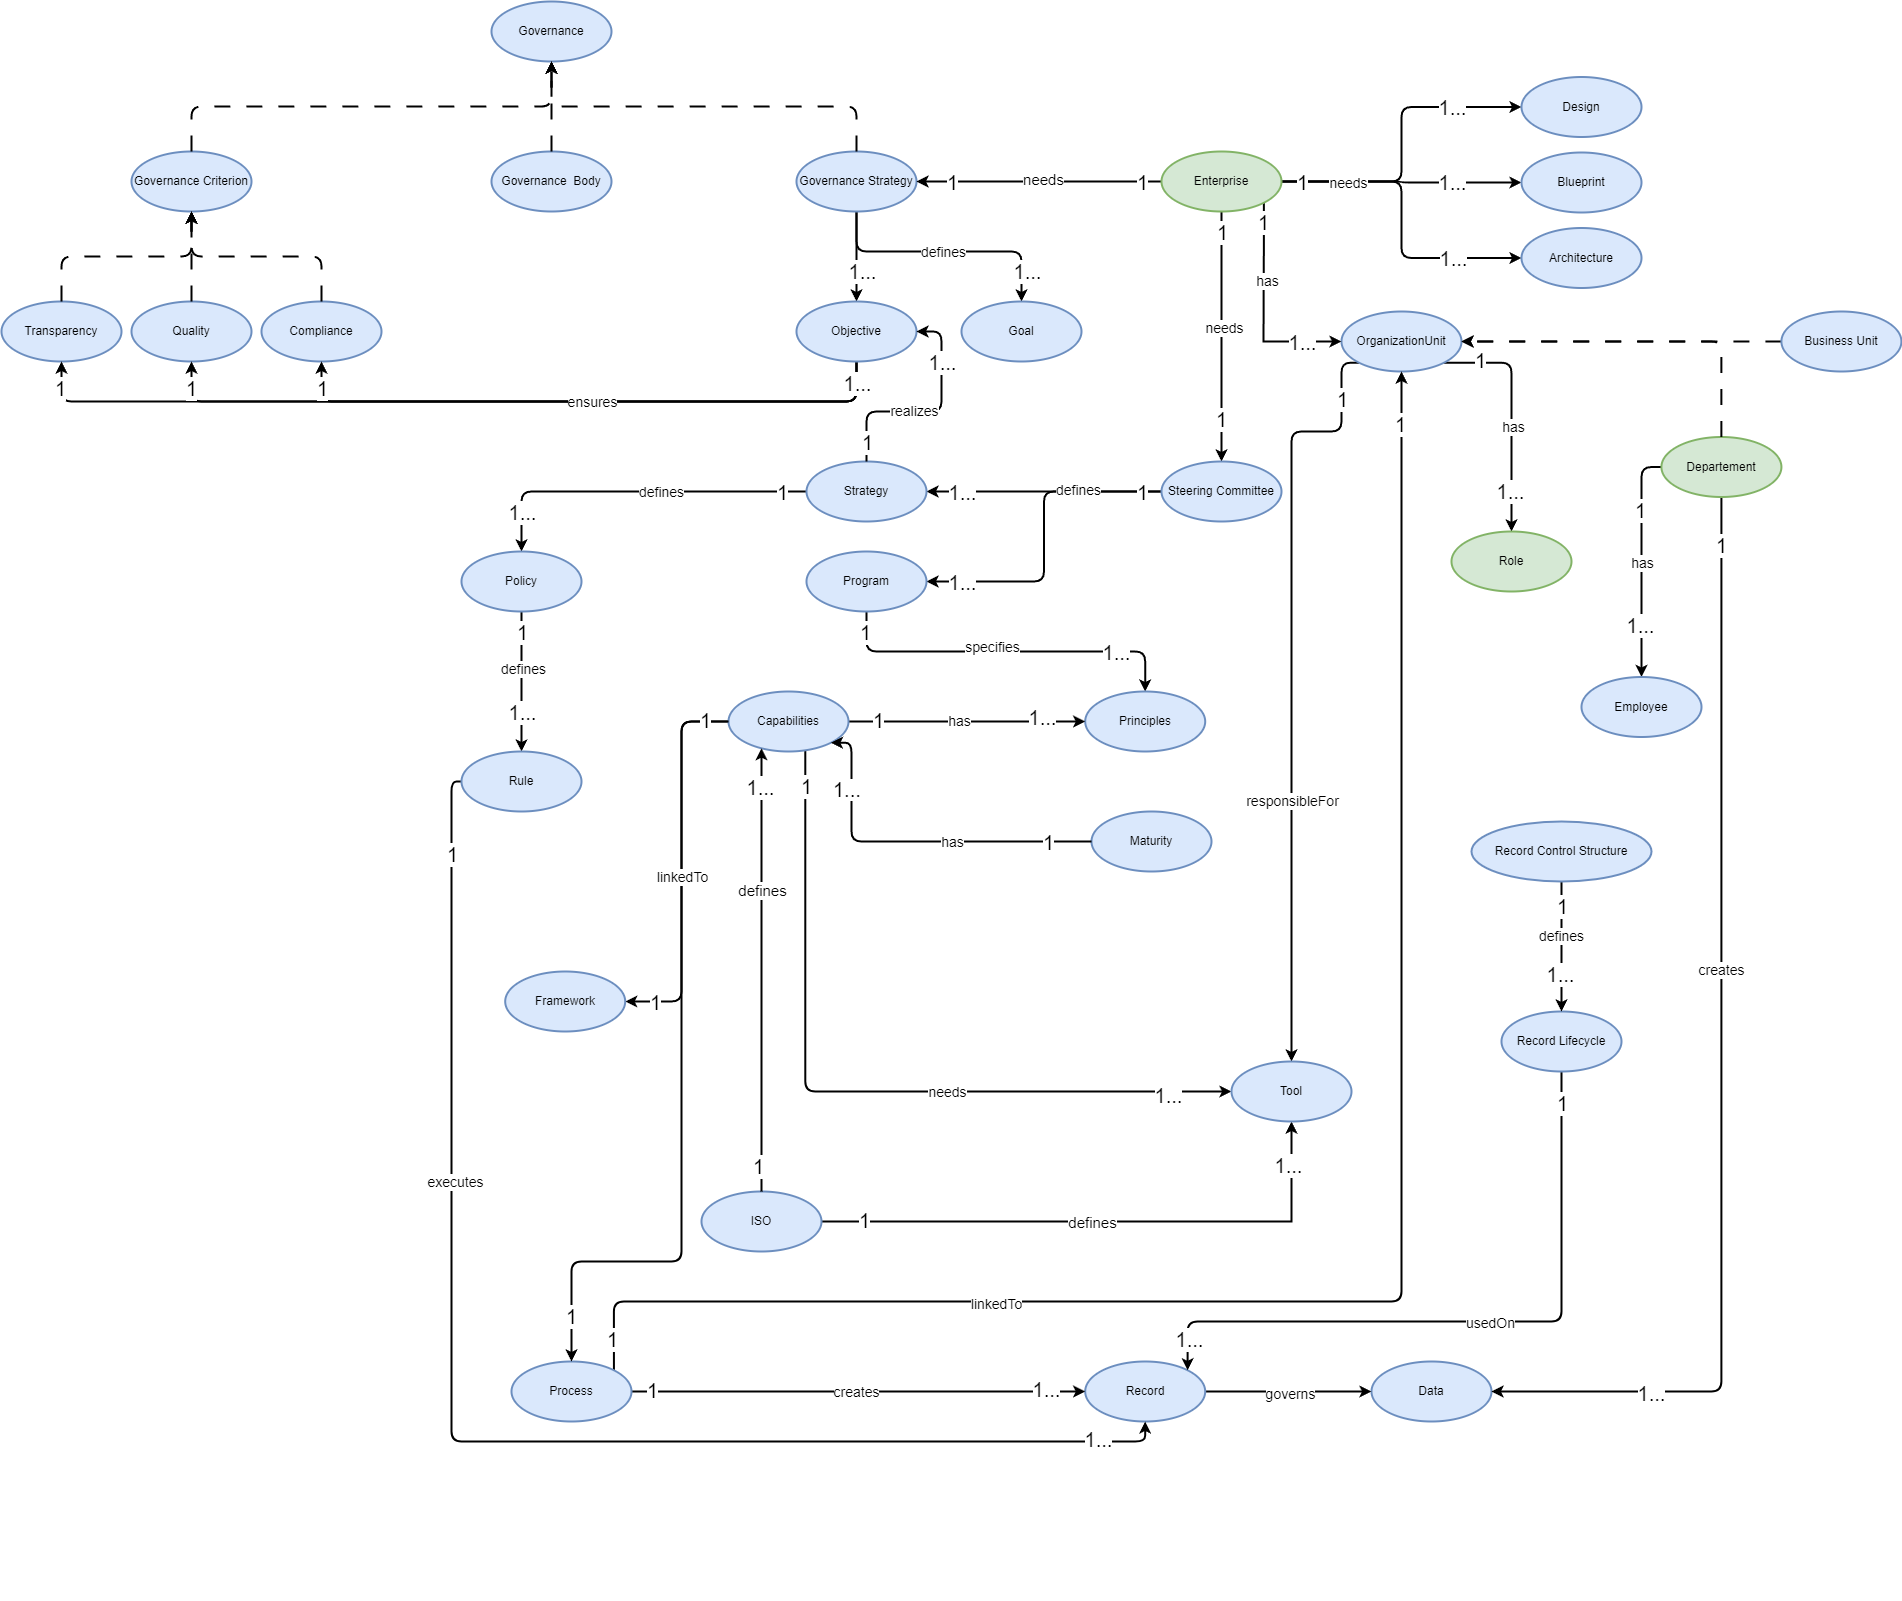
\includegraphics[width=\textwidth]{graphics/organization_overall.drawio.png}
  \caption{Visualization of the organization ontology.}
  \label{fig:organization}
\end{figure}

\section{Lifecycle Ontology}

The Lifecycle ontology is a relatively smaller one and focuses on the lifecycle of data, extending the organization ontology in the \textit{Record Lifecycle}. \textit{Data drives} the \textit{Record Lifecycle}, which handles the creation, management and retention of records. A well defined information lifecycle and its governance is crucial to reduce data growth, cost and risk, while optimizing the value of information \cite{Lambrechts2014Information}. \\
The \textit{Record Lifecycle} is divided into \textit{Service} and \textit{Process}. A \textit{Service} is a set of activities to manage, access or utilize data or records (e.g. information). The set of activities include: 
\begin{itemize}
    \item \textit{Access}, representing methods to access information by authorized user.
    \item \textit{Find}, representing methods to locate specific information. 
    \item \textit{Rendering}, representing methods to convert information into usable formats.
    \item \textit{Retrieve}, representing methods to retrieve specific information from a database.
    \item \textit{Service Search}, representing methods to search and retrieve data based on specific queries or criteria.
    \item \textit{Session}, representing periods during which a user can interact with the system to access and manipulate data. 
    \item \textit{Submission}, representing methods to upload data into the system for later processing, management or storage.
\end{itemize}

A \textit{Process} is a sequence of steps to achieve a specific record or data management goal. These goals range between the creation of records to its disposal and are achieved by these Processes: 

\begin{itemize}
    \item \textit{Archive}, representing the preservation of information by transfering them into a long-term storage.
    \item Classify, representing the categorization of data and records based on predefined criteria.
    \item Index, representing the indexing of information to improve searchability. 
    \item Measure , representing the applying of pre-defined metrics on information to enhance efficiency and compliance. 
    \item Metric, representing standard units of measurement.
    \item Monitor, representing the oversight of data management to ensure functionality.
    \item Retain, representing the process to keeping information as long as required by policies or other requirements. 
    \item Search, representing the process to locating information.
    \item Secure, representing the implementation of security measurements to protect data and records from unauthorized access. 
\end{itemize}

\textit{Processes} \textit{create} \textit{Statistics}, providing various information about different aspects of record management. With the help of these \textit{Statistics}, \textit{Reportings} are \textit{produced}, to inform the upper management and assist them in  decision-making and compliance. 

\begin{figure}[h]
  \centering
  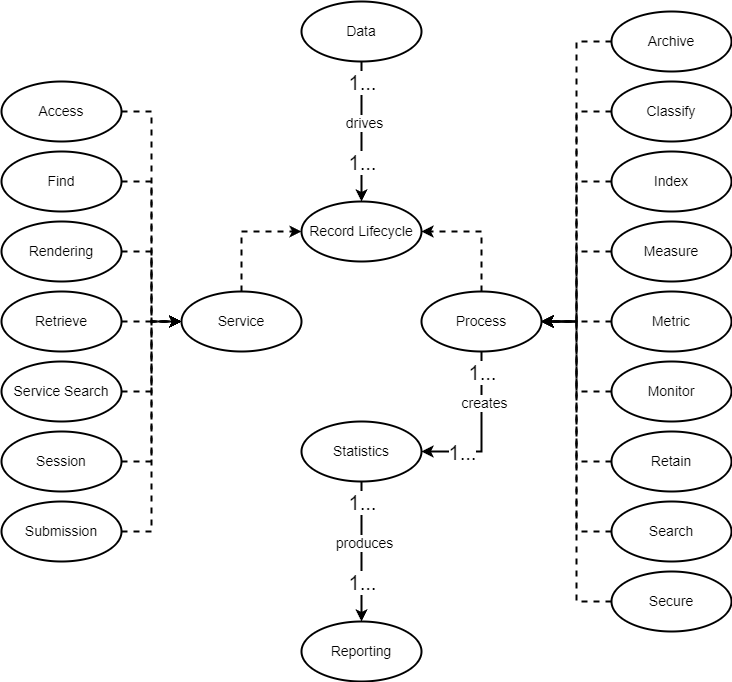
\includegraphics[width=0.7\textwidth]{graphics/lifecycle.drawio.png}
  \caption{Visualization of the lifecycle ontology.}
  \label{fig:lifecycle}
\end{figure}

\section{Information ontology}
The information ontology describes the concept of data and its information value. \textit{Data} represents raw facts used and collected by organizations and can be interpreted in many ways. \textit{Data} is \textit{equivalent to} an item, which represents a concrete individual unit of information. Every \textit{Item} has a \textit{Version} to represent its state over time. Since Data can have multiple structures, \textit{Document, Asset, Content} and \textit{Metadata} are defined as subclasses of \textit{Data}. \textit{Documents} are structured units of recorded information. A Document \textit{has} a \textit{Rendition}, which represents the document in a different format for a different purpose (different file format, different language, etc) and an \textit{Edition}, which documents updates and changes. \textit{Assets} describe strategic, financial or operational information valuable to the enterprise. \textit{Content} primarly focuses on the information conveyed by the Data itself. \textit{Metadata} provides \textit{Information} about Data, which is a subclass of \textit{Metadata}. This \textit{Information} can include \textit{Archival Information, Content Information} or a \textit{Description}. These pieces of \textit{Information} are \textit{contained in Files}, which in turn are \textit{contained in Container} - a broader term used for organizing and storing records. One example of a \textit{Container} are \textit{Folders}, used to group and organize files and their information. The \textit{Container} is a \textit{subclass of} \textit{Records}, indicating that it is part of the record-keeping system. The \textit{Record} class, directly connected to Data, is duplicated at the bottom of the graph due to overview reasons. \\
Every \textit{Data} can also be represented as a vector, comprising \textit{containing Value}, \textit{exposing Risk} and \textit{producing Cost}. Calculating these three components help decide how to handle the data in subsequent processes. For instance, data may be archived if its value is too low and the costs of retaining it in a repository are too high.\\

\textit{Records} \textit{classify} and therefore categorize and organize \textit{Data}, which is essential for effective data management \cite{Franks2013Records}. \textit{Records have} a \textit{Record Control Structure}, used to manage and control records within the organization. These \textit{Record Control Structures} include: 

\begin{itemize}
    \item \textit{Control Data}: Data used to manage the processing of often \textit{Sensitive Data}, such as \textit{Personnel Files, PII-Data, Audit Data, etc.}
    \item \textit{Report}: Data that provides information for analysis and decision-making. 
    \item \textit{Hold}: An organizational directory to retain records, often for audits or legal matters.
    \item \textit{Retention}: Policies to manage how long records should be kept.
    \item \textit{Audit Trail}:Recordings of changes or actions performed on records to ensure security, integrity and compliance \cite{Bjork1975Generalized}. 
    \item \textit{Category}: A classification of records. 
\end{itemize}

Every \textit{Record uses} a \textit{Data Dictionary}, which serves as a \textit{vocabulary for} the \textit{Taxonomy}, providing terms and definitions for a uniform categorization and classification within the taxonomy and therefore to effectively organize information \cite{Milne2007Taxonomy}. The Data Dictionary ensures consistency, clarity and is essential for effective record keeping \cite{Blethyn2008Data}.  \\

A \textit{Policy} is a set of guidelines to govern proceedings and activities within an enterprise. \textit{Policies grant Priviliges} to \textit{Roles}, defining what actions a role can perform.  \textit{Policies monitor metrics}, to evaluate their effectiveness and to enable necessary changes. A \textit{Policy has} a \textit{Goal}, representing an objective, a desired outcome or a principle like Accountability, that the policy aims to achieve. These policies and their goals need to be implemented. This is done by first \textit{applying Rules}, which are specific regulations that must be followed. These \textit{Rules} build the foundation and \textit{define} a \textit{Schedule}, which is \textit{used in Retention} to ensure that records are kept for a correct amount of time.

\begin{figure}[h]
  \centering
  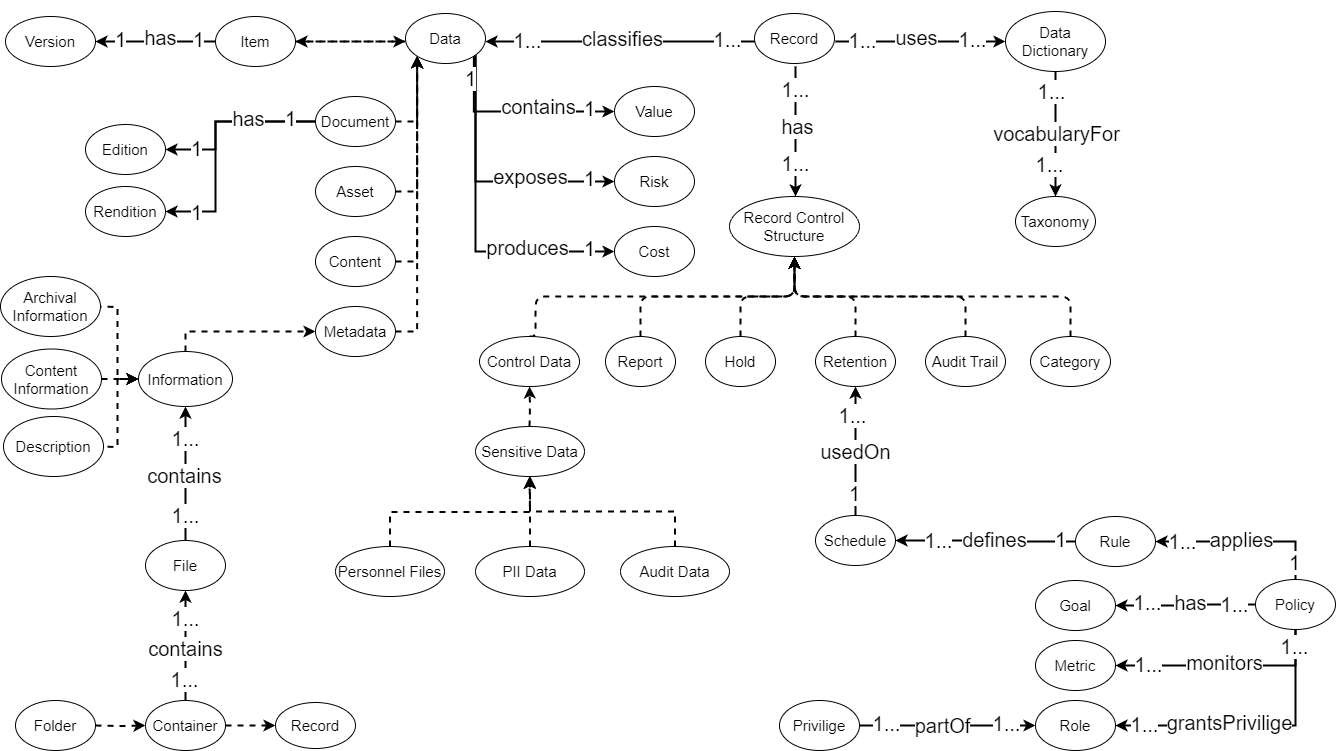
\includegraphics[width=\textwidth]{graphics/information.drawio.png}
  \caption{Visualization of the information ontology.}
  \label{fig:information}
\end{figure}

\section{\acrlong{SWRL} rules} \label{sec:SWRL}

The \acrshort{SWRL} rules are handled seperately in this Section, because some of them extend across multiple ontologies. Every \acrshort{SWRL} rule that is implemented will be described in this section. There are two different levels on how these rules are implemented. Every rule is first implemented as a Horn clause, which is afterwards translated into semantic and syntactic coherent OWL syntax based on the OWL RDF/XML exchange syntax. This way, the implementation of SWRL rules are made easier with Horn clauses while simultanously provide expressive power \cite{Horrocks2005OWL}. The first rule will include a more detailed description, including the OWL translated code to give a impression how the OWL code looks like, while others are just explained with the Horn clauses. This is because the translated code is often large and the horn clauses convey a better understanding. \\


\begin{lstlisting}[style=turtle, caption={OWL translation \cite{SHACL}}]
[ <http://swrl.stanford.edu/ontologies/3.3/swrla.owl#isRuleEnabled> "true"^^xsd:boolean ;
   rdfs:comment "" ;
   rdfs:label "S1" ;
   rdf:type <http://www.w3.org/2003/11/swrl#Imp> ;
   <http://www.w3.org/2003/11/swrl#body> [ rdf:type <http://www.w3.org/2003/11/swrl#AtomList> ;
                                           rdf:first [ rdf:type <http://www.w3.org/2003/11/swrl#IndividualPropertyAtom> ;
                                                       <http://www.w3.org/2003/11/swrl#propertyPredicate> <http://www.semanticweb.org/igonto/jurisdiction#capabilityInvolvesArticle> ;
                                                       <http://www.w3.org/2003/11/swrl#argument1> <http://www.semanticweb.org/igsonto/cap> ;
                                                       <http://www.w3.org/2003/11/swrl#argument2> <http://www.semanticweb.org/igsonto/article>
                                                     ] ;
                                           rdf:rest [ rdf:type <http://www.w3.org/2003/11/swrl#AtomList> ;
                                                      rdf:first [ rdf:type <http://www.w3.org/2003/11/swrl#IndividualPropertyAtom> ;
                                                                  <http://www.w3.org/2003/11/swrl#propertyPredicate> <http://www.semanticweb.org/igonto/jurisdiction#obligationInvolvesArticle> ;
                                                                  <http://www.w3.org/2003/11/swrl#argument1> <http://www.semanticweb.org/igsonto/obligation> ;
                                                                  <http://www.w3.org/2003/11/swrl#argument2> <http://www.semanticweb.org/igsonto/article>
                                                                ] ;
                                                      rdf:rest rdf:nil
                                                    ]
                                         ] ;
   <http://www.w3.org/2003/11/swrl#head> [ rdf:type <http://www.w3.org/2003/11/swrl#AtomList> ;
                                           rdf:first [ rdf:type <http://www.w3.org/2003/11/swrl#IndividualPropertyAtom> ;
                                                       <http://www.w3.org/2003/11/swrl#propertyPredicate> <http://www.semanticweb.org/igonto/jurisdiction#capabilityInvolvesObligation> ;
                                                       <http://www.w3.org/2003/11/swrl#argument1> <http://www.semanticweb.org/igsonto/cap> ;
                                                       <http://www.w3.org/2003/11/swrl#argument2> <http://www.semanticweb.org/igsonto/obligation>
                                                     ] ;
                                           rdf:rest rdf:nil
                                         ]
 ] .

\end{lstlisting}\label{lst:shacl_shapes}

\subsection{Jurisdiction rules}

The jurisdiction rules primarly deal with inferences regarding the \textit{Capabilities, Obligations, Rights} and \textit{Requirements}

\begin{quote}
\textbf{capabilityInvolvesArticle}(?capability, ?article)  $\land$  
\textbf{obligationInvolvesArticle}(?obligation, ?article) \\ $\rightarrow$ 
\textbf{capabilityInvolvesObligation}(?capability, ?obligation)
\end{quote}


\chapter{Evaluation}
\section{Use-Case Scenario}\label{sec:useCase}
\subsubsection{Use-Case description}
\subsubsection{Use-Case queries}

\section{Validation}

\section{Further Development}\label{sec:furtherDevelopment}
When finishing a prototype the question arises how the prototype affects future work and how well it can be integrated in further processes. Creating prototypes that are not just throwaway models but more an integral that form a final and functioning product is one of the main characteristics of evolutionary prototyping. The prototype is continuously refined and evolved based on feedback and requirements until it becomes the final product \cite{Boehm}. Evolutionary prototyping reduces risks (which is very important for an expert system that relies on compliance) \cite{sommerville2011software} and allows more flexibility and adaptability in design, as changes can be incorporated iteratively \cite{pressman2014software}.  \\  So the ability to reuse or to work further with a prototype is also a quality aspect and therefore part of this chapter. This section describes how this prototype can be integrated in an independent application and how certain design decisions are implemented to help developing an own application. \\

\subsection{Towards an IGONTO application}
Given that IGONTO is an expert system, there is a definitive need to develop a bespoke application or user interface for interacting with this ontology. This requirement became evident during the development of the prototype. For instance, to visualize query results, AllegroGraph was used in conjunction with Gruff. AllegroGraph is a scalable RDF Graph Database that supports big data analysis. Gruff, a visualization application, can utilize AllegroGraph as a database and visualize query results, allowing interaction with nodes in various ways \cite{FranzAllegroGraph}. While AllegroGraph enables querying with reasoning, it cannot incorporate the SWRL rules implemented in IGONTO. Therefore, to observe all inferences, the ontology must be materialized, saving all reasoning triples in the RDF graph before uploading to AllegroGraph. \\
To address this issue, we explored Stardog, another RDF Graph Database with visualization and querying capabilities. Stardog facilitates reasoning not only within its own application but also via its HTTP Endpoint. However, its visualization capabilities were limited, offering only a 'Query builder' that restricts query options like FILTER, and the reasoning process was slow. Stardog itself acknowledges that it 'performs reasoning in a lazy and late-binding fashion: it does not materialize inferences; rather, reasoning is performed at query time' \cite{Stardog}.\
This experience encountered during the development of IGONTO illustrates the challenge of finding services that fulfill all the requirements for IGONTO. Moreover, there are additional reasons to consider implementing a proprietary system for interfacing with the ontology:

\begin{enumerate}
    \item \textbf{Extensibility and Specification:} \\
    As previously mentioned, IGONTO is an expert system. It may require specific features not available in third-party services. Developing an application ensures independence and facilitates the easy implementation of specialized features as needed.
    
    \item \textbf{Integration:} \\
    Another advantage is the potential for integration into bigger and already existing systems. When integrating IGONTO into a larger system, reliance on third-party services can be limiting. The ability to tailor the application to specific needs enhances its integration capabilities within the broader system architecture.
    
    \item \textbf{Cost:} \\
    While the initial development of a custom application will lead to costs, it can be more economical in the long term. This is because most third-party services involve ongoing expenses, and it is unlikely that a single service will meet all of IGONTO's requirements, potentially leading to additional costs for multiple services. 

    \item \textbf{Useability:}\\
    A critical aspect of this discussion centers on user interaction. Information governance represents a complex domain, often unfamiliar to users seeking compliance guidance. These users may lack foundational knowledge in ontologies and their application. Even if they possess a rudimentary understanding of ontology interaction and SPARQL query formulation, they might not fully grasp the comprehensive range of factors necessary for compliance adherence. Consequently, even with a set of predefined SPARQL queries guiding through various use cases and their permutations, users could find it challenging to select appropriate queries accurately, because it may be not clear what Use-Case represents their situation.\\
    There are two potential solutions. The first involves the engagement of a domain expert who can facilitate user navigation through this complex process. However, this approach incurs ongoing costs. Alternatively, developing a user interface that enables intuitive interaction with the ontology, without requiring users to interact directly with the ontology structure and SPARQL queries, could be a more sustainable solution. This interface would ideally bridge the gap between the user's compliance needs and the technical demands of ontology management, thereby enhancing usability while reducing costs in the long term.
\end{enumerate}

Considering these points, a design concept will be presented that illustrates how a potential application might appear, how certain design decisions from the ontology will aid in the development of this application, and how some potentially desired features will enhance the system's quality. \\


\subsection{Application Design}

This section introduces a preliminary design proposal for the IGONTO application. Figure \ref{fig:systemdesign} illustrates the proposed system architecture, comprising a frontend for user interaction and a backend for data acquisition and processing. This architecture enables the frontend to effectively utilize processed data. The application's workflow is segmented into four subprocesses: Compliance Checklist, Data Gathering, Data Processing, and Results Presentation.\\

\begin{figure}
\centering
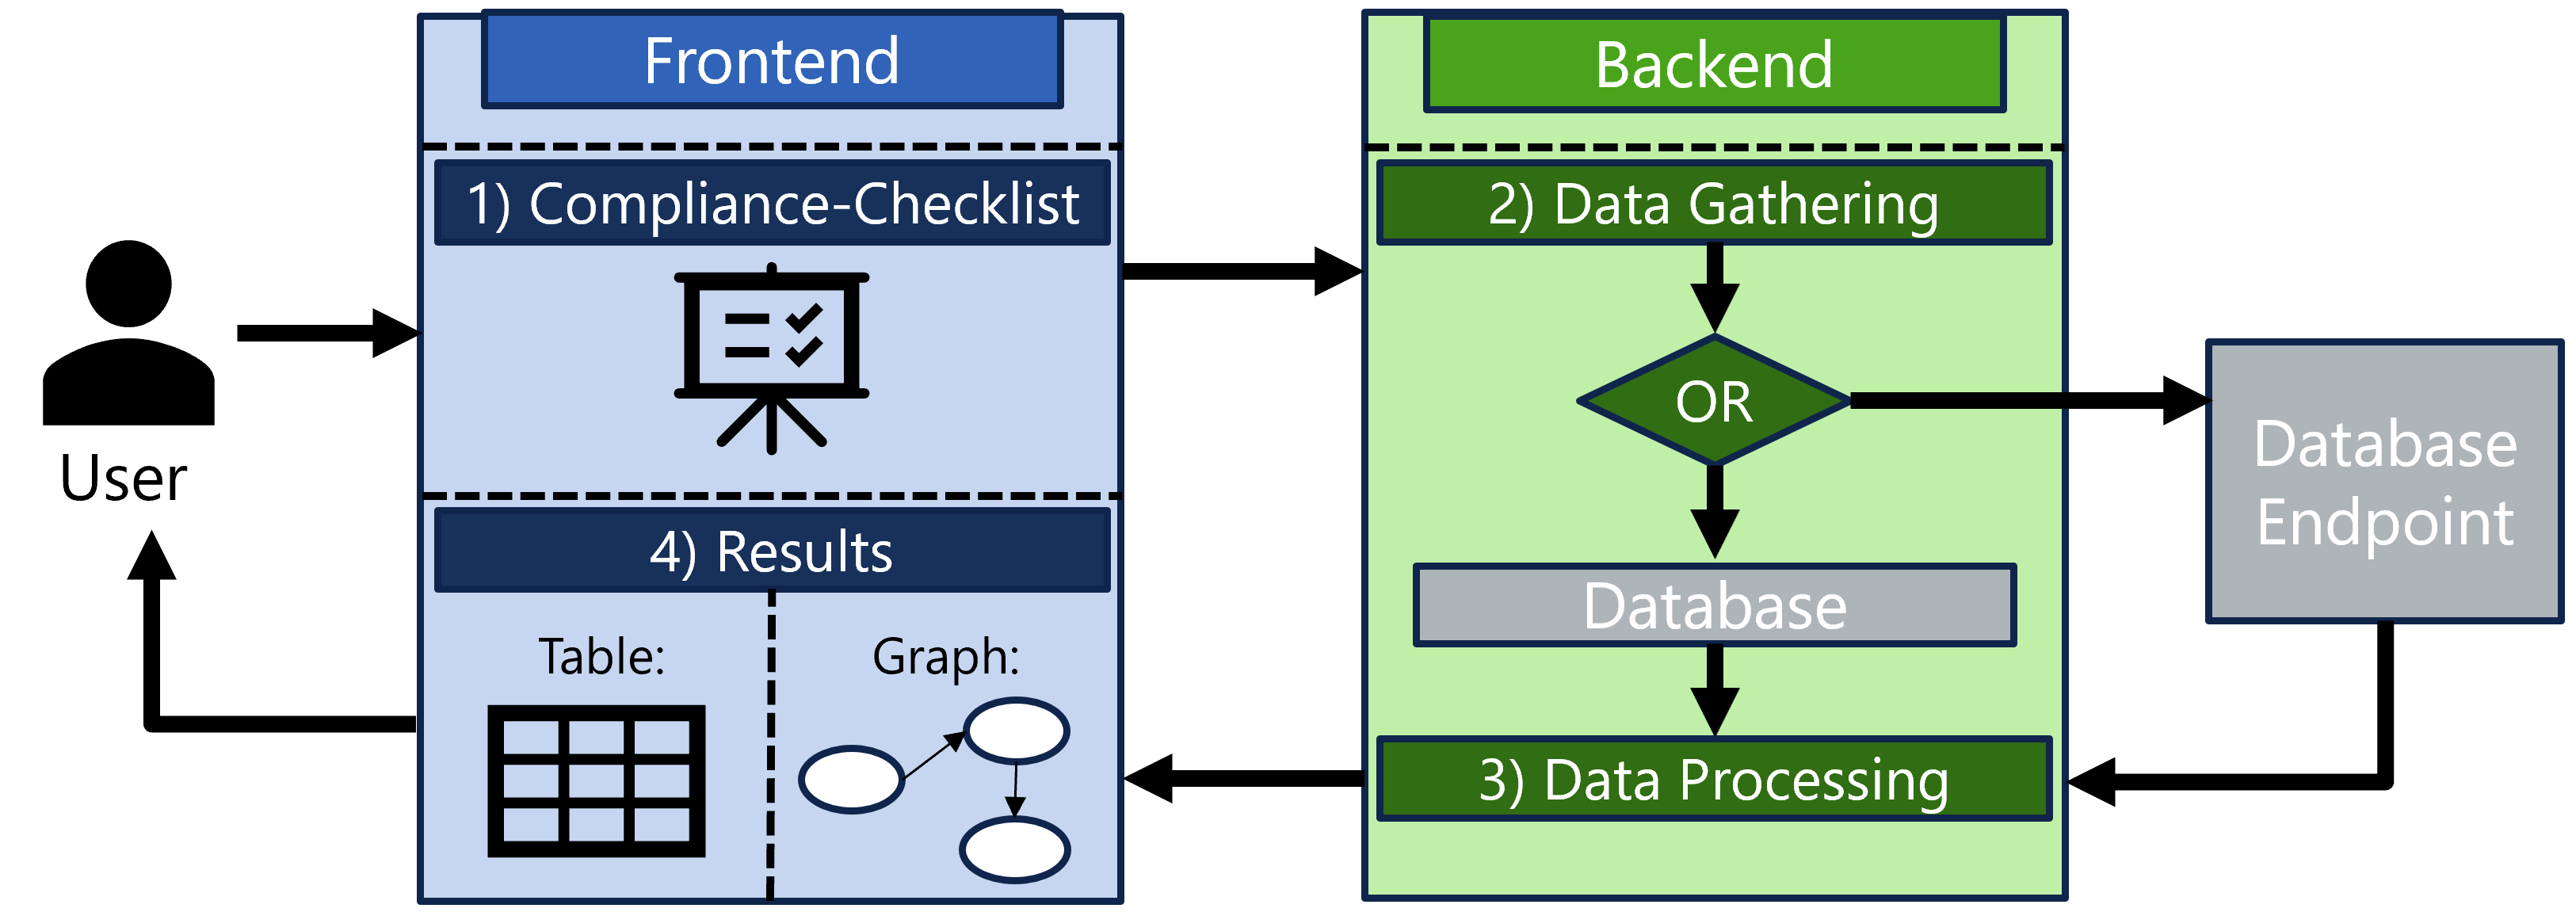
\includegraphics[width=\textwidth]{graphics/systemdesign.png}
\caption{Proposed system design for the IGONTO application.}
\label{fig:systemdesign}
\end{figure}

\subsubsection{Compliance Checklist}\label{sec:complianceChecklist}

The Compliance Checklist serves as the user's initial interaction point. Its primary function is to identify the user's specific use case, thereby guiding the subsequent data acquisition process. This is achieved through a series of predefined questions tailored to ascertain the precise use case. Key questions include:

\begin{enumerate}
    \item \textbf{What is the location of the company?} \\
    This question aims to categorize the company within the appropriate jurisdiction, establishing the regulatory framework applicable to the user. 
    \item \textbf{How many employees does the company have?}\\
    The size of the company is an important factor. For instance, companies with less than 250 employees have to comply to fewer regulations than large companies (see \ref{sec:useCase}).
    \item \textbf{Does the company deal with sensitive Data?}\\
    Handling sensitive data like \acrlong{PII} Data needs more caution and therefore influences the regulatory requirements.
    \item \textbf{How often is data processed / accessed?}\\
    The regularity of data processing impacts the compliance measures needed. There is a greater likelihood that additional measures will be necessary, when data is accessed more frequently.
\end{enumerate}

These are just example questions. A comprehensive checklist would include additional queries to cover all potential use cases. Moreover, the questions may vary based on the regulatory environment of the company's location. For example, U.S. regulations, not covered in this prototype, may necessitate different questions.\\
It would be beneficial if the answers were constrained to ensure that they encompass every potential use case, thereby limiting the combination possibilities in the backend. Suggested limitations for each question might include:
\begin{enumerate}
    \item  Provide a dropdown list of countries, similar to what is commonly found in other user applications.
    \item Allow the user to input an integer representing the company's employee count. Implementing corresponding ranges in the backend should be straightforward.
    \item Offer a checklist of data types that the company deals with, enabling the user to select multiple options.
    \item Include single choices such as 'once a year', 'once a month', etc., tailored to different compliance requirements based on processing frequency.
\end{enumerate}

Upon completion, the user's responses are forwarded to the backend for further processing.

\subsubsection{Data Gathering}
With all questions awnsered, the backend is able to determine the correct use-case by analysing the combinations awnsered from the checklist. Once the correct use-case is known, the backend either picks predefined SPARQL queries or dynamically generates queries based on the user's responses. These queries are then executed against the ontology to retrieve the necessary results. The database can either be accessed via its Endpoint, if it is hosted externally, or by integrating the ontology directly within the backend. A possible Database endpoint could be any online RDF Graph Databse. For example stardog, as previously mentioned. Stardog also provides a comprehensive HTTP API documentation \cite{StardogHTTPDocs}. \\
Alternatively, the database can be integrated and queried locally using RDFLib \cite{RDFLibDocs}, a Python framework designed for working with ontologies. RDFLib allows data to be serialized into graphs stored in memory, enabling queries to be executed and yielding results comparable to those obtained using an endpoint. Additionally, RDFLib supports reasoning and the pre-preparation of queries, which can enhance overall performance.\\
Either way, both methologies lead to the same results. 

\subsubsection{Data Processing}
After receiving the query results, the data needs to be processed for easy utilization by the frontend. These results can be in various formats such as CSV, JSON, XML, etc. The specific formats supported are detailed in the documentation of either Stardog or RDFLib. Listing \ref{lst:jsonResult} illustrates an example of a result in JSON format. This data now requires processing to ensure that the frontend can use it effortlessly, minimizing the need for additional processing.

\begin{lstlisting}[language=json,firstnumber=1]
    {
        "predicate": {
          "type": "uri",
          "value": "http://www.semanticweb.org/igonto/igonto#enterpriseDoesNotNeed"
        },
        "small_enterprise": {
          "type": "uri",
          "value": "http://www.semanticweb.org/igonto/organization#Small_Enterprise_Instance"
        },
        "object": {
          "type": "uri",
          "value": "http://www.semanticweb.org/igsonto/igsonto-complete#RIMSOlutionInstance"
        }
    },
    {
        "predicate": {
          "type": "uri",
          "value": "http://www.semanticweb.org/igonto/jurisdiction#operatesInCountry"
        },
        "small_enterprise": {
          "type": "uri",
          "value": "http://www.semanticweb.org/igonto/organization#Small_Enterprise_Instance"
        },
        "object": {
          "type": "uri",
          "value": "http://www.semanticweb.org/igonto/jurisdiction#Germany"
        }
    },
\end{lstlisting}\label{lst:jsonResult}

Listing \ref{lst:jsonResult} presents a code snippet from an example query that retrieves every connection from the instance 'small\_enterprise'. The properties are stored in the variable 'predicate', and the objects connected to the small enterprise are represented in the variable 'object'. This result is then processed as needed. However, to meaningfully interpret this code, additional context is required. This is where PropertyGroups become useful.\\
In the first triple, the predicate 'enterpriseDoesNotNeed' is an inference and a negative object property. This connection explicitly indicates that the small enterprise does not require a 'RIMSolutionInstance'. The second triple is a static property, stating that the small enterprise operates in Germany. Without further modifications, it is challenging to discern more meaning from this result, such as determining whether a property is an inference or is intended to be a negative object property. In the result, both are simply listed as properties, making it difficult for the frontend to differentiate between them.\\
This scenario exemplifies the utility of ObjectProperties defined in section \ref{sec:PropertyGroups}. By grouping object properties, we imbue them with additional knowledge, which can be leveraged in the application to introduce enhanced features. The potential uses of these in the frontend are discussed later in section \ref{sec:resultRepresentation}. While it is theoretically possible to store all object properties in a hardcoded dictionary, the organization of data should ideally be managed by the ontology rather than the application itself. By implementing PropertyGroups, they can also be queried, enhancing the richness of the results. The outcome for 'enterpriseDoesNotNeed' and its 'objectGroup' is illustrated in listing \ref{lst:jsonResult2}.
   

\begin{lstlisting}[language=json,firstnumber=1]
      {
        "predicate": {
          "type": "uri",
          "value": "http://www.semanticweb.org/igonto/igonto#enterpriseDoesNotNeed"
        },
        "small_enterprise": {
          "type": "uri",
          "value": "http://www.semanticweb.org/igonto/organization#Small_Enterprise_Instance"
        },
        "objectGroup": {
          "type": "uri",
          "value": "http://www.semanticweb.org/igonto/igonto#InferenceObjectPropertyGroup"
        },
        "object": {
          "type": "uri",
          "value": "http://www.semanticweb.org/igsonto/igsonto-complete#RIMSOlutionInstance"
        }
      },
      {
        "predicate": {
          "type": "uri",
          "value": "http://www.semanticweb.org/igonto/igonto#enterpriseDoesNotNeed"
        },
        "small_enterprise": {
          "type": "uri",
          "value": "http://www.semanticweb.org/igonto/organization#Small_Enterprise_Instance"
        },
        "objectGroup": {
          "type": "uri",
          "value": "http://www.semanticweb.org/igonto/igonto#NegativeObjectPropertyGroup"
        },
        "object": {
          "type": "uri",
          "value": "http://www.semanticweb.org/igsonto/igsonto-complete#RIMSOlutionInstance"
        }
      },
\end{lstlisting}\label{lst:jsonResult2}

One drawback of this method is, that if an object property is grouped in two PropertyGroups, the overall information connected to the object duplicated, because the variable 'objectGroup' contains two values. However, the issue can be solved by concatenating both values into one string using the 'GROUP\_CONCAT' operation from SPARQL. The downside of this method is, that afterwards the string needs to be separated again. Additionally, there are not many object properties involved in a single which makes it unlikely to lead to performance issues. The overall knowledge acquisition from these PropertyGroups outweighs the drawbacks they present.\\
Once when data is processed into suitable results, it will be returned to the frontend for further processing.  

\subsubsection{Result Representation}\label{sec:resultRepresentation}
When the results are processed in a way that it will be easy to deal with, they should be presented in a user friendly way to awnsers the questions compliance and implementation needs. One suggestions is, that the results can be presented in a tabular format and as an interactive RDF graph. The tabular representation  provides quick and direct information, while the graph should visualize the result for a better understanding. The idea is to allow the user to interact with the graph, such as expanding existing nodes for deeper searches and also to be able to visually distinguish between certain connections. A design concept is illustrated in figure \ref{fig:visualizationDesign}. The earlier metnioned Object PropertyGroups can now be acitvely visualized in the graph and filtered as using the selection options in the top right corner. The user now can choose to view only inferences, only negative relationships, only normal relationships or any other possible combination of these three options.This approach enables the easy representation of more knowledge allowing the user precisely to understand what they do not need to do by selecting only negative Object Property Groups. This leads to a better useability and overall performance. \\

Another use of a Object PropertyGroup namely the "InverseObjectPropertyGroup" allows users to expand nodes and to automatically retrieve the correct hierarchy, enhancing understandability. Meanhwhile the apllication uses the same generic query with the only difference that the subject is changed (namely, the selected instance that the user wished to expand). This way, the query can be imeplemented as single resuable query, that asks for all connections with their corresponding PropertyGorup, all objects that connected by this relationship and then the inverse relationship ("the way back"). The application then determines which relationship between subject and object is an inverse property and decides , based on the user's selection and desired hierarchy (e.g. top down, bottom up or both ways) how the data is displayed. This approach results in an automatic generated tree structure, without the requirememt for the application to be aware of every relationship and object. Without this method, the application would be limited to only predefined SPARQL queries, restricting the users ability to interact with the graph as wished.\\


\begin{figure}
\centering
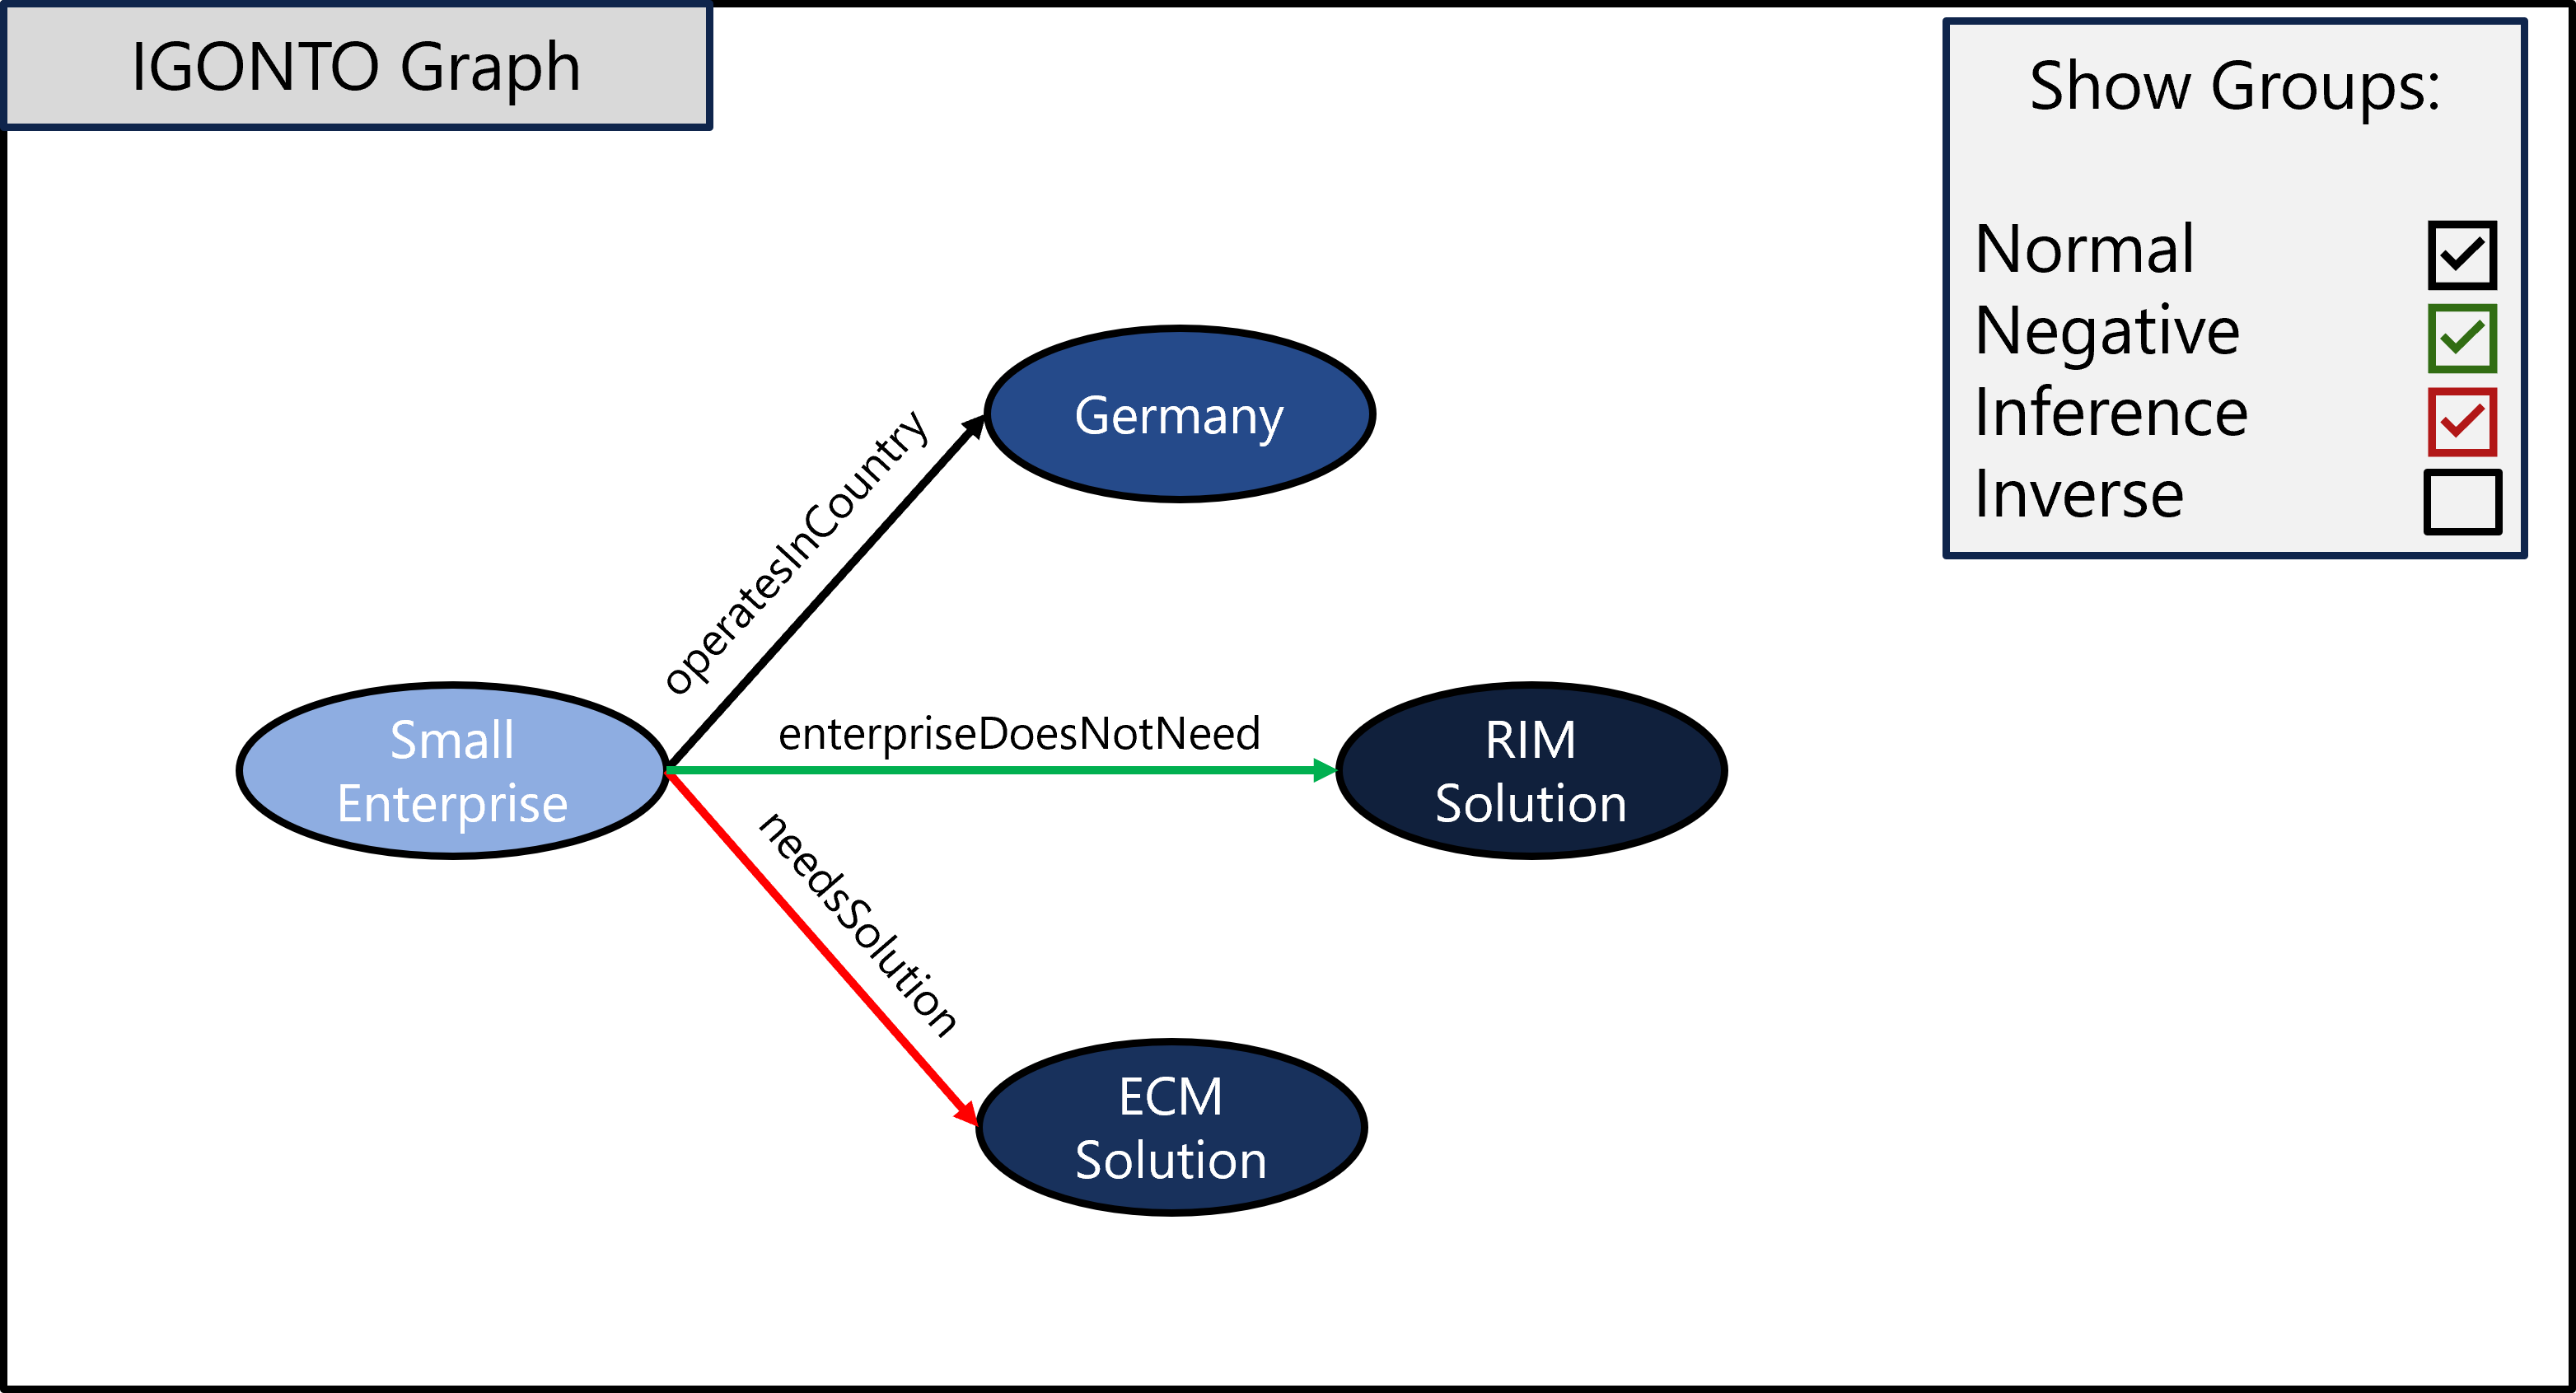
\includegraphics[width=\textwidth]{graphics/graphDesign.png}
\caption{Graph visualization design concept for the IGONTO application.}
\label{fig:visualizationDesign}
\end{figure}

\subsection{Agile Development}

While the previous section focused on integrating the IGONTO prototype into an independent application, this section shifts attention to how the further development of this prototype can be managed within an agile team. The division of IGONTO into several independent subontologies outlined in section \ref{sec:ontology_hierarchy} plays a crucial role for the agile development for agile development. Additonaly, the capability to store RDF graphs into different named graphs is utilized in this idea. A named graph is basically a set of triples with a specific name, based on a certain ontology. Named graphs facilitate the organization of RDF data into different subsets. These subsets can be inrements from each other or different viewpoins.\\
Figure \ref{fig:agileIGONTO} illustrates how the prototype can be developed by different teams. Each subontology can be developed by an independet person or department. The various lines represent different branches in the development process. The overall ontology can be saved into the 'Master' branch. Whenever a pull request is created, the corresponding graph can be validated and, if successful, saved as a named graph in the database. The graphs can be named based on the development branch and the pull request number to uniquely identify each graph and trace every change. Upon merging into the master branch, a new master graph also can be stored in the database as a named graph with an increment of the version number. The integration of a new pull request or merge into a new named graph can be automated using workflow files, just like the validation of every ontology. \\
The exact implementation depends on the database used. When using Stardog, its HTTP API enables the direct integration of new named graphs. With RDFlib, these named graphs need to be stored into the \textit{Dataset} object provided by RDFlib. Withing this dataset, several named graphs can be integrated. \\

\begin{figure}
\centering
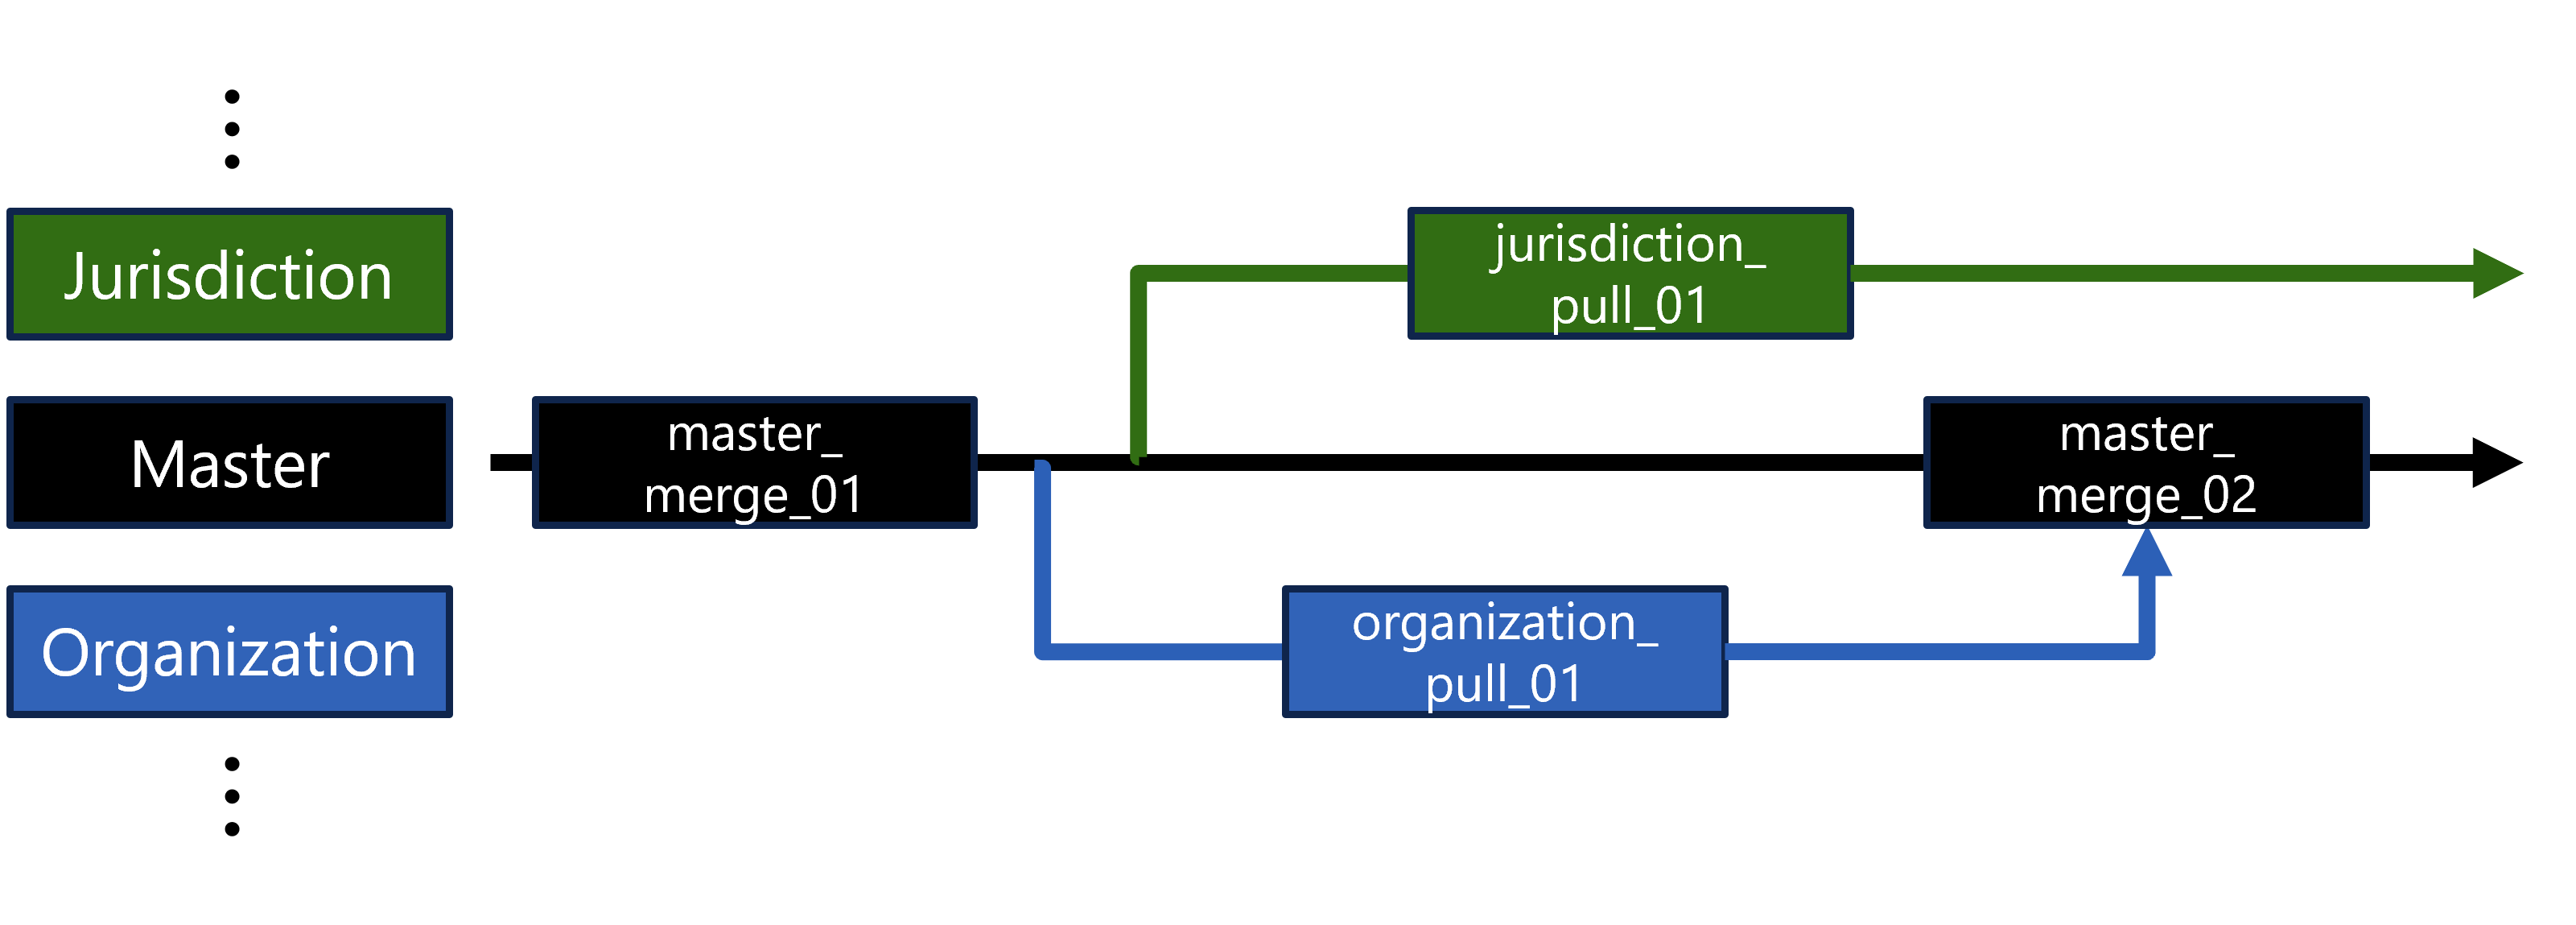
\includegraphics[width=\textwidth]{graphics/agileDesign.png}
\caption{Agile development of IGONTO.}
\label{fig:agileIGONTO}
\end{figure}

\chapter{Outlook}
The IGONTO prototype has shown considerable potential but still needs some improvements to be fully operational. This chapter outlines some improvements to achieve compliance, including the Refinement \ref{sec:Refinement} and the Use case extension \ref{sec:Use case extension}. Additionally, the possible improvements to show the potential of this prototype explained in section \ref{sec:furtherDevelopment} are summarized to provide a comprehensive outlook.

\section{Refinement}\label{sec:Refinement}

The structure of the prototype is already robust, including the division of ontologies, the description logic, the \acrshort{SWRL} rules and the validation. The primary focus of refinement involves the connection between requirements, rights, obligations and GDPR articles. \\

\begin{figure}
\centering
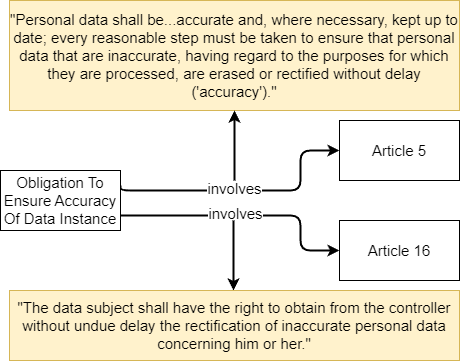
\includegraphics[width=0.6\textwidth]{graphics/refinement.drawio.png}
\caption{Refinement reason example}
\label{fig:refinement}
\end{figure}

As explained in Section \ref{sec:jurisdictionOntology} obligations, rights and capabilities are linked to GDPR articles. Figure \ref{fig:refinement} illustrates on why and where refinement should be carried out. The instance \textit{Obligation To Ensure Accuracy Of Data Instance} involves \textit{Article 5} and \textit{Article 16} including a citation from the articles, explaining why the relationship is existent in the first place. Sometimes, like in \textit{Article 5}, the citations are straightforward and directly include keywords ('accuracy') with their explanation. Here, the involvement of \textit{Article 5} in this obligation is clear. At Other times, out-of-the-box explanations are necessary to connect the articles. For instance, \textit{Article 16} states,  \begin{quote}
``The data subject shall have the right to obtain from the controller without undue delay the rectification of inaccurate personal data concerning him or her.''
\end{quote}
Here, the connection to the obligation is not immediately apparent. This article obligates controllers to correct inaccuracies in personal data. But to be able to correct these inaccuracies, the data must be kept accurate. Otherwise, rectification will be challenging or could lead to errors within their data, potentially resulting in compliance violations. \\
This demonstrates that its often not clear which articles are relevant to obligations, rights or capabilities. Although it was not a requirement for this prototype to be compliant but to show that the idea of the whole process works, the need for refinement should still be mentioned. IGONTO is an expert system that requires a high degree of accuracy to ensure compliance and therefore definitely should be revised by (data compliance) experts. \\   

\section{Use Case extension}\label{sec:Use case extension}
The use case extension is another task that needs to be completed. In this first prototype, we focused on the size of enterprises to demonstrate that the idea works. There are more use cases and parameters that play a role in compliance. Some additional use cases have been identified but not implemented and are briefly mentioned in Section \ref{sec:complianceChecklist}.\\

The first additional use case is the type of data the enterprise processes. If the data is sensitive, such as \acrshort{PII} data, more security and therefore stricter regulations need to be followed. The other use case is the frequency of data processing. These parameters also have to be added to the ontolog, including the right connections and inferences. Although we did not directly implement these use cases, the concept is already implemented. For example, in Figure \ref{fig:information}, the sensitive data is already implemented as type of control data. The frequency of data access can be implemented by attributes or by adding an additional class that represents the concept of Date, including a start date, end date and other subclasses required to implement a process cycle.\\
Beside the already identified but not implemented use cases, there could be more use cases needed to ensure compliance. As mentioned earlier, IGONTO is an expert system and should be revised by experts, not only regarding article refinement but also regarding use case extension.

\chapter{Related Work}

Describe relevant scientific literature related to your work.

\chapter{Conclusion}
\label{chap:zusfas}


\printbibliography

All links were last followed on March 17, 2018.

\appendix

\pagestyle{empty}
\renewcommand*{\chapterpagestyle}{empty}
\Versicherung
\end{document}
